\RequirePackage[thinlines]{easybmat} %-- muss aufgrund eines Bugs vor etex und tikz geladen werden
\documentclass[a4paper, twoside, headsepline, index=totoc,toc=listof, fontsize=10pt, cleardoublepage=empty, headinclude, DIV=13, BCOR=13mm, titlepage,]{scrartcl}
\usepackage{scrtime} % KOMA, Uhrzeit ermoeglicht
\usepackage{scrpage2} % wie fancyhdr, nur optimiert auf KOMA-Skript, leicht andere Syntax
\usepackage{etoolbox}
\usepackage{letltxmacro}

% Compiler abhaengige IFs
\usepackage{ifxetex,ifluatex}
\newif\ifxetexorluatex
\ifxetex
  \xetexorluatextrue
\else
  \ifluatex
    \xetexorluatextrue
  \else
    \xetexorluatexfalse
  \fi
\fi

%--Farbdefinitionen
%-- muss vor tikz geladen werden
\usepackage[usenames, table, x11names]{xcolor}
\definecolor{dark_gray}{gray}{0.45}
\definecolor{light_gray}{gray}{0.6}

%--Zum Zeichnen
%-- muss vor polyglossia bzw. babel geladen werden
\usepackage{tikz}
\usepackage{tikz-cd}
\usetikzlibrary{external}
\tikzset{>=latex}
\usetikzlibrary{shapes,arrows,intersections}
\usetikzlibrary{calc,3d}
\usetikzlibrary{decorations.pathreplacing,decorations.markings}
\usetikzlibrary{angles}

%-- Konfiguration von tikzexternalize
\tikzexternalize[prefix=tikz/, up to date check=diff]

\ifxetexorluatex
\tikzset{external/system call={xelatex \tikzexternalcheckshellescape %-- verwende LuaLaTeX, wegen dynamischer Speicherallokation
    -halt-on-error -interaction=batchmode -jobname "\image" "\texsource"}}
\else
\tikzset{external/system call={pdflatex \tikzexternalcheckshellescape 
    -halt-on-error -interaction=batchmode -jobname "\image" "\texsource"}}
\fi

%-- tikzexternalize fuer tikzcd deaktivieren, da inkompatibel
\AtBeginEnvironment{tikzcd}{\tikzexternaldisable}
\AtEndEnvironment{tikzcd}{\tikzexternalenable}

%-- um Inkompatibilitaeten von quotes und polyglossia bzw. babel zu vermeiden
\tikzset{
  every picture/.append style={
    execute at begin picture={\shorthandoff{"}},
    execute at end picture={\shorthandon{"}}
  }
}
\usetikzlibrary{quotes}
\usepackage{pgfplots}
\usepgfplotslibrary{colormaps}
\pgfplotsset{compat=1.10}



%-- Mathe
\usepackage{mathtools} % beinhaltet amsmath
\mathtoolsset{showonlyrefs, centercolon}
\newtagform{brackets}[\textbf]{[}{]}
\usetagform{brackets}
\usepackage{wasysym}
\usepackage{amssymb} %zusätzliche Symbole
\usepackage{latexsym} %zusätzliche Symbole
\usepackage{stmaryrd} %für Blitz
\usepackage{nicefrac} %schräge Brüche
\usepackage{cancel} %Befehle zum Durchstreichen
\usepackage{mathdots}
% \usepackage{bm}
\DeclareSymbolFont{bbold}{U}{bbold}{m}{n}
\DeclareSymbolFontAlphabet{\mathbbold}{bbold}
\newcommand{\mathds}[1]{\mathbb{#1}} %Um Kompatibilitaet mit frueheren Benutzung von dsfont herzustellen
\newcommand{\ind}{\mathbbold{1}} % charakteristische-Funktion-Eins
\def\mathul#1#2{\color{#1}\underline{{\color{black}#2}}\color{black}} %farbiges Untersteichen im Mathe-Modus

%-- Alles was mit Schrift und XeteX zu tun hat
\ifxetexorluatex
    % XeLaTeX or LuaTeX
	\ifxetex
		\usepackage{mathspec} %beinhaltet fontspec 
	\else
		\usepackage[no-math]{fontspec}
	\fi
    \usepackage{polyglossia} %babel-ersatz
    \setmainlanguage[spelling=new,babelshorthands=false]{german}
	\newcommand\glqq{"}
	\newcommand\grqq{"}
	\defaultfontfeatures{Mapping=tex-text, WordSpace={1.4}} %
    \setmainfont[Ligatures=Common, BoldFont={* Bold}, ItalicFont={* Light Italic},SmallCapsFont={Linux Libertine O}, SmallCapsFeatures={Letters=SmallCaps}]{Source Sans Pro}
	\setsansfont[Scale=MatchLowercase,Ligatures=Common, BoldFont={* Medium}]{Ubuntu}
	\ifxetex
		\setallmonofonts[Scale=MatchLowercase, ItalicFont={*}]{Consolas} 
	\else
		\setmonofont[Scale=MatchLowercase, ItalicFont={*}]{Consolas}
	\fi
	\usepackage{xltxtra}
	\usepackage{fontawesome}
	\usepackage{microtype}
\else
    % default: pdfLaTeX
    \usepackage[ngerman]{babel}
    \usepackage[T1]{fontenc}
    \usepackage[utf8]{inputenc}
	\usepackage{textcomp} %verhindert ein paar Fehler bei den Fonts
    \usepackage[babel=true, tracking=true]{microtype}
	\usepackage{lmodern}
	\renewcommand{\familydefault}{\sfdefault} 
\fi


%--Mixed
\usepackage[neverdecrease]{paralist}
\usepackage[german=quotes]{csquotes}
\usepackage{makeidx}
\usepackage{booktabs}
\usepackage{wrapfig}
\usepackage{float}
\usepackage[margin=10pt, font=small, labelfont={sf, bf}, format=plain, indention=1em]{caption}
\captionsetup[wrapfigure]{name=Abb. }
\usepackage{stackrel}
\usepackage{ifthen}
\usepackage{multicol}
\usepackage{qrcode}
\flushbottom

%--Hyphenation
\hyphenation{di-men-si-o-na-le}


%--Unterstreichung
\usepackage[normalem]{ulem}
\setlength{\ULdepth}{1.8pt}

%--Indexverarbeitung
\newcommand{\bet}[1]{\textbf{#1}}
\newcommand{\Index}[1]{\textbf{#1}\index{#1}}
\makeindex
\setindexpreamble{{\noindent \itshape Die \emph{Seitenzahlen} sind mit Hyperlinks zu den entsprechenden Seiten versehen, also anklickbar} \ifxetexorluatex \faHandUp\fi \par \bigskip}
\renewcommand{\indexpagestyle}{scrheadings}


%--Marginnote & todonotes
\usepackage{marginnote}
\renewcommand*{\marginfont}{\color{dark_gray} \itshape \footnotesize }
\usepackage[textsize=small]{todonotes}

%--Todonotes mit tikz/externalize kompatibel machen
\LetLtxMacro{\oldtodo}{\todo}
\renewcommand{\todo}[2][]{\tikzexternaldisable\oldtodo[#1]{#2}\tikzexternalenable}
\LetLtxMacro{\oldmissingfigure}{\missingfigure}
\renewcommand{\missingfigure}[2][]{\tikzexternaldisable\oldmissingfigure[{#1}]{#2}\tikzexternalenable}

%--Konfiguration von Hyperref pdfstartview=FitH, 
\usepackage[hidelinks, pdfpagelabels,  bookmarksopen=true, bookmarksnumbered=true, linkcolor=black, urlcolor=SkyBlue2, plainpages=false,pagebackref, citecolor=black, hypertexnames=true, pdfauthor={Jannes Bantje}, pdfborderstyle={/S/U}, linkbordercolor=SkyBlue2, colorlinks=false]{hyperref}

% \let\orighref\href
\ifxetexorluatex
\newcommand{\hrefsym}[2]{\href{#1}{\texttt{#2\,\faExternalLink}}}
\newcommand{\hrefsymmail}[2]{\href{#1}{\texttt{\faEnvelope\,#2}}}
\renewcommand{\url}[1]{\hrefsym{#1}{\nolinkurl{#1}}}
\fi
\providecommand{\hrefsym}{\href}
% \usepackage{cleveref}
% \crefformat{footnote}{#2\footnotemark[#1]#3}

%--Römische Zahlen
\newcommand{\RM}[1]{\MakeUppercase{\romannumeral #1{}}}

%--Punkte (nach hyperref)
\usepackage{ellipsis}

%%--Abkürzungen etc.
\newcommand{\light}{\text{\Large $\lightning$}}

%-- Definitionen von weiteren Mathe-Befehlen
\DeclareMathOperator{\re}{Re} %Realteil
\DeclareMathOperator{\im}{Im} %Imaginaerteil
\DeclareMathOperator{\id}{id} %identische Abbildung
\DeclareMathOperator{\Sp}{Sp} %Spur
\DeclareMathOperator{\sgn}{sgn} %Signum
\DeclareMathOperator{\alt}{Alt} %Alternierende n-linearFormen
\DeclareMathOperator{\End}{End} %Endomorphismen
\DeclareMathOperator{\Vol}{Vol} %Volumen
\DeclareMathOperator{\dom}{dom} %Domain
\DeclareMathOperator{\Hom}{Hom} %Homomorphismen
\DeclareMathOperator{\bild}{Bild} %Bild
\DeclareMathOperator{\Kern}{Kern }
\DeclareMathOperator{\rg}{rg} %Rang
\DeclareMathOperator{\Rg}{Rg} %Rang
\DeclareMathOperator{\diam}{diam} %Durchmesser
\DeclareMathOperator{\dist}{dist} %Distanz
\DeclareMathOperator{\grad}{grad} %Gradient
\DeclareMathOperator{\dive}{div} %Gradient
\DeclareMathOperator{\rot}{rot} %Rotation
\DeclareMathOperator{\hess}{Hess} %Hesse-Matrix
\DeclareMathOperator{\koker}{Koker} %Kokern
\DeclareMathOperator{\aut}{Aut} %Automorphismen
\DeclareMathOperator{\ord}{ord} %Ordnung
\DeclareMathOperator{\ggT}{ggT} %ggT
\DeclareMathOperator{\kgV}{kgV} %kgV
\DeclareMathOperator{\Gr}{Gr} %Gerade
\DeclareMathOperator{\Kr}{Kr} %Kreis
\DeclareMathOperator{\Char}{char} %Charakteristik
\DeclareMathOperator{\Aut}{Aut} %Automorphismen
% \DeclareMathOperator{\D}{D} %formale Ableitung
\newcommand{\D}{\ensuremath{\mathrm{D}\mkern-1.5mu}}
\newcommand{\mathd}{\ensuremath{\mathrm{d}\mkern-1.0mu}}
\newcommand{\Tmap}{\ensuremath{\mathrm{T}\mkern-1.0mu}}
\newcommand{\opL}{\ensuremath{\mathrm{L}\mkern-0.6mu}}
\DeclareMathOperator{\cov}{cov} %Kovarianz
\DeclareMathOperator{\Gal}{Gal} %Galois
\DeclareMathOperator{\supp}{supp} %Träger
\DeclareMathOperator{\Sym}{Sym} %Symmetrische Gruppe
\DeclareMathOperator{\Zyl}{Zyl} %Zylinder
\DeclareMathOperator{\Mod}{Mod} %Moduln
\DeclareMathOperator{\EPK}{EPK} %Einpunktkompaktifizierung
\DeclareMathOperator{\conj}{conj} %Konjugation
\DeclareMathOperator{\ann}{ann} %Annulator
\DeclareMathOperator{\tor}{tor} %Torsionsmodul
\DeclareMathOperator{\Int}{Int} %Interior/Inneres
\DeclareMathOperator{\Br}{Br} %Brauerergruppe
\DeclareMathOperator{\GL}{GL} %allgemeine lineare Gruppe
\DeclareMathOperator{\SL}{SL} %spezielle lineare Gruppe
\DeclareMathOperator{\SU}{SU} %spezielle unitäre Gruppe
\DeclareMathOperator{\Tr}{Tr} %Spur/Trace
\DeclareMathOperator{\conv}{conv} %Konvexe Teilmenge
% \DeclareMathOperator{\tr}{tr}
\newcommand{\tr}{\mathrm{tr}}
\newcommand{\w}{\mathrm{w}}
\newcommand{\weakT}[1]{\ensuremath{\mathcal{T}_{#1}^{\mkern+1.0mu\text{\raisebox{0.4ex}{$\mathrm{w}$}}}}}
\newcommand{\weakTstar}[1]{\ensuremath{\mathcal{T}_{#1}^{\mkern+1.0mu\text{\raisebox{0.4ex}{$\mathrm{w}$}}^*}}}
\newcommand{\rand}[1]{\ensuremath{\partial^{\scriptscriptstyle #1}}}


% -- Kategorien
\DeclareMathOperator{\Ob}{Ob} %Objekte
\DeclareMathOperator{\Mor}{Mor} %Morphismen

% \DeclareMathOperator{\TOP}{TOP} %Topologische Räume
\newcommand{\TOP}{\textsc{Top}}
% \DeclareMathOperator{\HTOP}{HTOP} %Topologische Räume + Homotopieäquivalenz
\newcommand{\HTOP}{\textsc{HTop}}
% \DeclareMathOperator{\VR}{VR} %Vektorräume
\newcommand{\VR}{\textsc{VR}}
% \DeclareMathOperator{\MOD}{MOD} %Moduln
\newcommand{\MOD}{\textsc{Mod}}
% \DeclareMathOperator{\MENGEN}{MENGEN} %Mengen
\newcommand{\MENGEN}{\textsc{Mengen}}
% \DeclareMathOperator{\MAN}{MAN} %Mannigfaltigkeiten
\newcommand{\MAN}{\textsc{Man}}
% \DeclareMathOperator{\GRUPPEN}{GRUPPEN} %Gruppen
\newcommand{\GRUPPEN}{\textsc{Gruppen}}
% \DeclareMathOperator{\ABELGRUPPEN}{ABEL.GRUPPEN} %abelsche Gruppen
\newcommand{\ABELGRUPPEN}{\textsc{Abel.Gruppen}}
% \DeclareMathOperator{\KAT}{KAT} %Kategorien
\newcommand{\KAT}{\textsc{Kat}}
% \DeclareMathOperator{\FUN}{FUN} %Funktoren
\newcommand{\FUN}{\textsc{Fun}}


\newcommand{\op}{\mathrm{op}}

\newcommand{\Ker}{\ensuremath{\Kern \,}}
\newcommand{\zirkel}{\rotatebox[origin = c]{-90}{$\varangle$}}
\newcommand{\wirkung}{\!\curvearrowright\!}

\newcommand{\oE}{\OE}

%--Beweisende
\newcommand{\bewende}{\ifmmode \tag*{$\square$} \else \hfill $\square$ \fi}

%--Volumen
\newcommand{\vol}[1]{\ensuremath{\Vol_{#1}}}

%--Skalarprodukt
\DeclarePairedDelimiterX\sprod[2]{\langle}{\rangle}{#1\,\delimsize\vert\,#2}

%--Betrag, Gaußklammer
\DeclarePairedDelimiter{\abs}{\lvert}{\rvert}
\DeclarePairedDelimiter{\ceil}{\lceil}{\rceil}

%--Norm
\DeclarePairedDelimiter\doppelstrich{\Vert}{\Vert}
\newcommand{\norm}[2][\relax]{
\ifx#1\relax \ensuremath{\doppelstrich*{#2}}
\else \ensuremath{\doppelstrich*{#2}_{#1}}
\fi}


%--Umklammern
\DeclarePairedDelimiter\enbrace{(}{)}
\DeclarePairedDelimiter\benbrace{[}{]}
\DeclarePairedDelimiter\lenbrace{<}{>}

%--Mengen
\DeclarePairedDelimiterX\mengenA[1]{\lbrace}{\rbrace}{#1}
\DeclarePairedDelimiterX\mengenB[2]{\lbrace}{\rbrace}{#1\, \delimsize\vert \, #2}

\makeatletter
\newcommand{\set}[2][\relax]{
\ifx#1\relax \ensuremath{
\mengenA*{#2}}
\else \ensuremath{%
  \mengenB*{#1}{#2}}
\fi}
\makeatother


%--offen und abgeschlossen
\newcommand{\off}{\! \stackrel[\text{offen}]{}{\subset} \!}
\newcommand{\abg}{\! \stackrel[\text{abg.}]{}{\subset} \!}

%--Differential
\newcommand{\diff}[2]{\ensuremath{\frac{{\partial #1}}{{\partial #2}} }}
\newcommand{\diffd}[2]{\ensuremath{\frac{\mathd #1}{\mathd #2} }}

%--Diagonale Linien für Matrizen
\newcommand\tikzmark[1]{%
  \tikzexternaldisable\tikz[overlay,remember picture,baseline] \node [anchor=base] (#1) {};\tikzexternalenable}

\newcommand\MyLine[3][]{%
  \tikzexternaldisable\begin{tikzpicture}[overlay,remember picture]
    \draw[#1] (#2.south) -- (#3.north);
  \end{tikzpicture}\tikzexternalenable}
  
%--Jordankasten
\newcommand{\Jord}{ \tikzexternaldisable \begin{BMAT}{|ccc|}{|ccc|} %
				0 & & \\ %
				1\tikzmark{z} &  \diagdown & \\ %
				& \tikzmark{u}1 \MyLine[thick]{z}{u} &  0 %
			\end{BMAT} \tikzexternalenable}
			
%--Jordankasten mit Lambda
\newcommand{\JordLa}[1][\empty]{%
	\tikzexternaldisable\ifthenelse{\equal{#1}{\empty}}
		{\begin{BMAT}{|ccc|}{|ccc|} %
				\lambda & & \\ %
				1\tikzmark{z} &  \diagdown & \\ %
				& \tikzmark{u}1 \MyLine[thick]{z}{u} &  \lambda  %
			\end{BMAT}}
		{\begin{BMAT}{|ccc|}{|ccc|} %
				\lambda_{#1}  & & \\ %
				1\tikzmark{z} &  \diagdown & \\ %
				& \tikzmark{u}1 \MyLine[thick]{z}{u} &  \lambda_{#1}  %
			\end{BMAT}}\tikzexternalenable}

%--Inhaltsverzeichnis
\usepackage[tocindentauto]{tocstyle}
\usetocstyle{KOMAlike}			

\newcommand{\fach}{Lineare Algebra \RM{2}}
\newcommand{\semester}{SoSe 2013}
\newcommand{\homepage}{http://wwwmath.uni-muenster.de/reine/u/topos/lehre/SS2013/LineareAlgebra2/index.html}
\newcommand{\prof}{Prof.\,Dr.\,Arthur Bartels}
\providecommand{\verfasser}{Jannes Bantje}

%--Konfiguration von scrheadings
\setheadsepline{1pt}[\color{light_gray}]
\pagestyle{scrheadings}
%\fancyhf[H, F]{}
\clearscrheadfoot

\providecommand{\shortFach}{\fach}
\lehead{ 
\includegraphics[height=0.5 cm,keepaspectratio]{../!config/Bilder/Logo_WWU_Muenster_light_gray.pdf}}
\rehead{\rule{0cm}{0.5cm}\footnotesize \sffamily \color{light_gray} \verfasser -- Mitschrift \shortFach}
\lohead{\rule{0cm}{0.5cm} \footnotesize \sffamily \color{light_gray} Stand: \today \; \thistime[:]}
\rohead{
\includegraphics[height=0.5 cm,keepaspectratio]{../!config/Bilder/fb10logo_gray.pdf}}


\ofoot[{ \color{dark_gray} \LARGE \sffamily \thepage}]{{ \color{dark_gray} \LARGE \sffamily \thepage}} %hier wir auch der plain Stil bearbeitet!
\automark{section}
\ifoot{ \color{dark_gray} \small \leftmark}

%--Metadaten
\author{\verfasser}
\titlehead{
\includegraphics[height=1.5cm, keepaspectratio]{../!config/Bilder/Logo_WWU_Muenster.pdf}%
\hfill 
\includegraphics[height=1.3cm, keepaspectratio]{../!config/Bilder/fb10logo.pdf}}
\title{Skript \fach}
\subtitle{Mitschrift der Vorlesung  \enquote{\fach} von \prof}

\publishers{
Aktuelle Version verfügbar bei: \bigskip\\
\normalsize
\begin{minipage}[t]{0.45\textwidth}
	\centering{
	\qrcode[height=3.5cm, version=4]{https://github.com/JaMeZ-B/latex-wwu}
	\medskip\\
	
\includegraphics[height=0.4cm, keepaspectratio]{../!config/Bilder/github_octo.pdf} 
	
\includegraphics[height=0.4cm, keepaspectratio]{../!config/Bilder/GitHub_Logo.pdf} (inklusive Sourcecode)\\
	{\small\url{https://github.com/JaMeZ-B/latex-wwu}}}
\end{minipage}
\hfill
\begin{minipage}[t]{0.45\textwidth}
	\centering{
	\qrcode[height=3.5cm, version=4]{btsync://B6WH2DISQ5QVYIRYIEZSF4ZR2IDVKPN3I?n=latex_share}
	\medskip\\
	
\includegraphics[height=0.4cm, keepaspectratio]{../!config/Bilder/bt_sync_logo.pdf} 
	{\large \textbf{Bittorrent} Sync} \\
	\texttt{B6WH2DISQ5QVYIRYIEZSF4ZR2IDVKPN3I}
	}
\end{minipage}
}



\begin{document}
\pagenumbering{Roman}
\maketitle
\begin{abstract}
\section*{Vorwort --- Mitarbeit am Skript}
Dieses Dokument ist eine Mitschrift aus der Vorlesung \enquote{\fach, \semester}, gelesen von \prof. Der Inhalt entspricht weitestgehend dem Tafelanschrieb. Für die
Korrektheit des Inhalts übernehme ich keinerlei Garantie! Für Bemerkungen und Korrekturen -- und seien es nur Rechtschreibfehler -- bin ich sehr dankbar. 
Korrekturen lassen sich prinzipiell auf drei Wegen einreichen: 
\begin{itemize}
	\item Persönliches Ansprechen in der Uni, Mails an \hrefsymmail{mailto:\mail}{\mail} (gerne auch mit annotieren PDFs) 
	\item \emph{Direktes} Mitarbeiten am Skript: Den Quellcode poste ich auf GitHub (siehe oben), also stehen vielfältige Möglichkeiten der Zusammenarbeit zur Verfügung:
	Zum Beispiel durch Kommentare am Code über die Website und die Kombination Fork + Pull Request. Wer sich verdient macht oder ein Skript zu einer Vorlesung, die 
	ich nicht besuche, beisteuern will, dem gewähre ich gerne auch Schreibzugriff.
	
	Beachten sollte man dabei, dass dazu ein Account bei \url{github.com} notwendig ist, der allerdings ohne Angabe von persönlichen Daten angelegt werden kann. 
	Wer bei GitHub (bzw. dem zugrunde liegenden Open-Source-Programm \enquote{\texttt{git}}) -- verständlicherweise -- Hilfe beim Einstieg braucht, dem helfe ich gerne 
	weiter. Es gibt aber auch zahlreiche empfehlenswerte Tutorials im Internet.\footnote{zB. \url{https://try.github.io/levels/1/challenges/1}, ist auf Englisch, aber dafür 
	interaktives LearningByDoing}
	\item \emph{Indirektes} Mitarbeiten: \TeX-Dateien per Mail verschicken. 
	
	Dies ist nur dann sinnvoll, wenn man einen ganzen Abschnitt ändern möchte (zB. einen alternativen Beweis geben), da ich die Änderungen dann per Hand einbauen muss! Ich freue mich aber auch über solche Beiträge!
\end{itemize}
\section*{Vorlesungshomepage}
{\centering 
\begin{minipage}[c][][c]{\textwidth}
	\centering \qrcode[height=3cm]{\homepage} \medskip\\
	\footnotesize \url{\homepage}
\end{minipage}
\par}

\end{abstract}

\setcounter{page}{1}
\tableofcontents
\cleardoubleoddemptypage
\pagenumbering{arabic}
\setcounter{page}{1}

% \tikzexternaldisable

\section{Isometrien} % (fold)
\label{sec:isometrien}

\subsection[Definition Isometrie]{Definition} % (fold)
\label{sub:definition11}
Sei $(V, \left\langle \, \mid \, \right\rangle )$ ein euklidischer oder unitärer Vektorraum. Ein Endomorphismus $f : V \to V$ heißt eine \Index{Isometrie}, falls für alle $v \in V$ gilt:
\[
	\| f(v) \|  =\| v \| \tag{\glqq Länge bleibt erhalten\grqq}
\] 
% subsection definition (end)

\subsection[Satz über Isometrie und das Skalarprodukt]{Satz} % (fold)
\label{sub:12}
\[
	f \text{ Isometrie } \iff \forall v,w \in V \text{ gilt } \left\langle f(v) \mid f(w) \right\rangle  = \left\langle v \mid w \right\rangle \quad (\star)
\]
\minisec{Beweis}
Gilt $(\star)$ so folgt
\[
	\| f(v) \|^2 = \left\langle f(v) \mid f(v) \right\rangle \underset{(\star)}{=} \left\langle v \mid v \right\rangle = \| v\|^2 
\]
Da $\| f(v) \| , \| v\| \ge 0$ folgt $\| f(v) \| = \|v\|$. Sei nun umgekehrt $f$ eine Isometrie. Für $v,w \in V$ gilt dann 
\[
	\left\langle f(v+w) \mid f(v+w) \right\rangle = \left\langle v+w \mid v+w \right\rangle 
\]
Also
\[
	\left\langle f(v) \mid f(v) \right\rangle + \left\langle f(v) \mid f(w) \right\rangle + \left\langle f(w) \mid f(v) \right\rangle + \left\langle f(w) \mid f(w) \right\rangle  = \left\langle v \mid v \right\rangle + \left\langle v \mid w \right\rangle + \left\langle w \mid v \right\rangle + \left\langle w \mid w \right\rangle 
\]
Wegen $\left\langle f(v) \mid f(v) \right\rangle = \left\langle v \mid v \right\rangle $ und $\left\langle f(w) \mid f(w) \right\rangle = \left\langle w \mid w \right\rangle $ folgt
\[
	\left\langle f(v) \mid f(w) \right\rangle + \left\langle f(w) \mid f(v) \right\rangle = \left\langle v \mid w \right\rangle + \sprod{w}{v} \tag{$\diamondsuit$}  
\]
Ist $V$ euklidisch so $\left\langle f(v) \mid f(w)	 \right\rangle = \left\langle f(w) \mid f(v) \right\rangle  $ und $\left\langle v \mid w \right\rangle = \left\langle w \mid v \right\rangle $ und es folgt $\left\langle f(v) \mid f(w) \right\rangle = \left\langle v \mid w \right\rangle $. Ist $V$ unitär so folgt nur 
\[
	\re \left\langle f(v) \mid f(w) \right\rangle = \re \left\langle v \mid w \right\rangle 
\]
Es gilt aber auch $\left\langle f(v+iw) \mid f(v+iw) \right\rangle = \left\langle v+ iw \mid v+iw \right\rangle $. Damit folgt analog zu ($\diamondsuit$)
\[
	\left\langle f(v) \mid i f(w) \right\rangle + \left\langle i(fw) \mid f(v) \right\rangle = \left\langle v \mid iw \right\rangle + \left\langle iw \mid v \right\rangle 
\]
Also
\begin{align*}
	-i \left\langle f(v) \mid f(w) \right\rangle + i \left\langle f(w) \mid f(v) \right\rangle &= -i \left\langle v \mid w \right\rangle + i \left\langle w \mid v \right\rangle \\
	\left\langle f(v) \mid f(w) \right\rangle - \left\langle f(w) \mid f(v) \right\rangle &= \left\langle v \mid w \right\rangle - \left\langle w \mid v \right\rangle
	\tag{Multiplikation mit $i$} 
\end{align*}
Es folgt $\im \left\langle f(v) \mid f(w) \right\rangle = \im \left\langle v \mid w \right\rangle $ \hfill \( \square \)
% subsection satz (end)

\subsection[Bemerkung für eine Orthonormalbasis]{Bemerkung} % (fold)
\label{sub:13}
Sei $e_1, \ldots , e_n$ eine Orthonormalbasis \index{Orthonormalbasis} von $V$ und $f \in \End(V)$. Dann ist $f$ genau dann eine Isometrie, wenn gilt
\[
	\sprod{f(e_i)}{f(e_j)} = \delta_{ij} \qquad \text{ für } i,j = 1, \ldots , n
\]
% subsection bemerkung (end)

\subsection[Satz über Isometrie und Matrizenprodukt]{Satz} % (fold)
\label{sub:satz14}
Sei $B= (e_1, \ldots , e_n)$ eine Orthonormalbasis und $f \in \End(V)$. Sei $A= m_B^B(f)$ Dann gilt:
\[
	f \text{ ist Isometrie } \iff A \cdot \overline{A}^t = I_n 
\]
\minisec{Beweis}
Es ist $A= (a_{ij})$ mit $a_{ij} = \left\langle f(e_j) \mid e_i \right\rangle $ da $f(e_j)= \sum_{i=1}^{n} \left\langle f(e_j) \mid e_i \right\rangle e_i$ ist.
Sei $f$ eine Isometrie. Dann 
\begin{align*}
	A \cdot \overline{A}^t &= \left( \sum_{j=1}^{n} \left\langle f(e_j) \mid e_i \right\rangle  \overline{\left\langle f(e_j) \mid e_k \right\rangle }  
	\right)_{ik} =: (b_{ik})_{ik}
\end{align*}
Da $f$ eine Isometrie ist, ist $f(B)= f(e_1), \ldots , f(e_n)$ auch eine Orthonormalbasis und es folgt
\begin{align*}
	b_{ik} &= \sum_{j=1}^{n} \sprod{f(e_j)}{e_i}  \left\langle e_k \mid f(e_j) \right\rangle \tag{Bilinearität}\\
	&= \sprod{\sum_{j=1}^{n} \left\langle e_k \mid f(e_j) \right\rangle  f(e_j)}{e_i} \tag{$e_k$ da $f(B)$ ONB ist} \\
	&= \left\langle e_k \mid e_i \right\rangle = \delta_{ki}
\end{align*}
Sei $A \cdot \overline{A}^t= I_n $. Dann ist auch $\overline{A}^t \cdot A = I_n $ und wir erhalten für alle $i,k$
\begin{align*}
	\sum_{j=1}^{n} \overline{\left\langle f(e_i) \mid e_j \right\rangle } \left\langle f(e_k) \mid e_j \right\rangle  = \delta_{ik}
\end{align*}
Es folgt
\begin{align*}
	\left\langle f(e_k) \mid f(e_i) \right\rangle &= \sprod{\sum_{j=1}^{n} \left\langle f (e_k) \mid e_j \right\rangle e_j}
	{\sum_{j=1}^{n} \left\langle f(e_i) \mid e_j \right\rangle e_j} \\
	&= \sum_{j=1}^{n} \left\langle f(e_k) \mid e_j \right\rangle \overline{\left\langle f(e_i) \mid e_j \right\rangle } \\
	&= \delta_{ik}
\end{align*}
\hfill \( \square \)
% subsection satz (end)

\subsection[Korollar über die Determinante einer Isometrie]{Korollar} % (fold)
\label{sub:korollar15}
Ist $f$ eine Isometrie \index{Isometrie} eines endlich dimensionalen euklidischen oder unitären Vektorraums, so ist
\[
	| \det f | = 1
\]
\minisec{Beweis}
Sei $B$ Orthonormalbasis von $V$, $A=m_B^B(f)$. Dann 
\[
	\det f = \det A  =\det A^t  = \overline{\det \overline{A}^t }
\]
Nach \ref{sub:satz14} folgt 
\[
	\det f \cdot  \overline{\det f} = \det A \cdot \det \overline{A}^t = \det (A \cdot  \overline{A}^t )  = \det (I_n) = 1 
\]
Also $|\det f | = 1$ \hfill \( \square \)

% subsection korollar (end)

\subsection[Lemma über die Gruppe der Isometrien]{Lemma} % (fold)
\label{sub:lemma16}
Sei $V$ euklidischer oder unitärer Vektorraum. Seien $f,g : V \to V$ Isometrien
\begin{enumerate}[a)]
	\item $f \circ g$ ist eine Isometrie
	\item $f$ ist injektiv \hfill {\color{light_gray} $\Rightarrow $ surjektiv, wenn $\dim V < \infty$}
	\item Ist $f$ bijektiv, so ist auch $f ^{-1}$ eine Isometrie
\end{enumerate}
Insbesondere bilden die Isometrien eine Gruppe, falls $\dim V < \infty$
\minisec{Beweis}
\begin{enumerate}[a)]
	\item $\| f \circ g (v) \| \underset{f \text{ Isometrie}}{=} \| g(v) \| \underset{g \text{ Isometrie}}{=} \| v\|$
	\item Sei $f(v)= 0 \Longrightarrow \| v \| = \| f(v) \| = \| 0\| = 0 \rightarrow v=0$
	\item $\| f ^{-1} (v) \| = \| f \left( f ^{-1} (v) \right) \| = \| v \|$
\end{enumerate}
\hfill \( \square \)
% subsection lemma16 (end)

\subsection[Definition orthogonale/unitäre Gruppe]{Definition} % (fold)
\label{sub:definition17}
\begin{enumerate}[(i)]
	\item Sei $V$ eine endlich dimensionaler euklidischer Vektorraum
	\[
		O(V) := \{ f \in \End(V) \mid f \text{ Ist Isometrie} \}
	\]
	heißt die \Index{orthogonale Gruppe} von $V$. Die Untergruppe 
	\[
		SO(V) := \{ f \in O(V) \mid \det f = 1 \}
	\] 
	heißt die \Index{spezielle orthogonale Gruppe} von $V$. Ist $V=\mathds{R}^n$ mit dem Standard-Skalarprodukt, so schreiben wir auch $O(n):= O(\mathds{R}^n)$ bzw
	$SO(n) := SO(\mathds{R}^n)$
	\item Sei $V$ eine endlich dimensionaler unitärer Vektorraum
	\[
		U(V) := \{ f \in \End(V) \mid f \text{ ist Isometrie} \}
	\]
	heißt die \Index{unitäre Gruppe} von $V$. Die Untergruppe 
	\[
		SU(V) := \{ f \in U(V) \mid \det f = 1 \}
	\] 
	heißt die \Index{spezielle unitäre Gruppe} von $V$. Ist $V=\mathds{C}^n$ mit dem Standard-Skalarprodukt, so schreiben wir auch $U(n):= U(\mathds{C}^n)$ bzw
	$SU(n) := SU(\mathds{C}^n)$
\end{enumerate}
% subsection definition17 (end) 

\subsection[Bemerkung über die Spalten der Matrizen in $O(n)$]{Bemerkung} % (fold)
\label{sub:18}
Wegen \ref{sub:13} ist $O(n)$ die Menge der Matrizen deren Spalten eine Orthonormalbasis von $\mathds{R}^n$ (mit Standardskalarprodukt) bilden. $U(n)$ ist die Menge der
Matrizen deren Spalten eine Orthonormalbasis von $\mathds{C}^n$ (mit Standardskalarprodukt) bilden.
% subsection 18 (end)

\subsection[Beispiel für (spezielle) orthogonale Gruppen]{Beispiel} % (fold)
\label{sub:19}
\begin{align*}
	O(2) &= {\set[\begin{pmatrix} a & - \varepsilon b \\ b & \varepsilon a \end{pmatrix}]{a^2 + b^2 =1 , \varepsilon \in \{ \pm 1 \}} }\\
	SO(2) &= {\set[\begin{pmatrix} a & -  b \\ b &  a \end{pmatrix}]{a^2 + b^2 = 1 \enspace a,b \in \mathds{R}} = \set[\begin{pmatrix} \cos \varphi & - \sin \varphi \\ \sin \varphi & \cos \varphi \end{pmatrix}]{\varphi \in [0, 2 \pi )}}
\end{align*}
% subsection 19 (end)

\subsection[Bemerkung über \glqq drehende\grqq Isometrie ]{Bemerkung} % (fold)
\label{sub:110}
$D(\varphi) := \begin{pmatrix}
	\cos \varphi & - \sin \varphi \\
	\sin \varphi & \cos \varphi
\end{pmatrix}$ wirkt als Drehung um den Winkel $\varphi$ um den Nullpunkt auf $\mathds{R}^2$.
% subsection 110 (end)

\subsection[Beispiel einer spiegelnden Isometrie]{Beispiel} % (fold)
\label{sub:111}
Sei 
\[
	S= \begin{pmatrix}
		1 & 0 \\
		0 & -1
	\end{pmatrix} \in O(2)\setminus SO(2)
\]
$S$ wirkt als Spiegelung an der Achse $e_1$. Es ist $S^2 = I_2$. Es gilt $O(2)= SO(2) \cup SO(2) \cdot S$. Jedes Element in $SO(2) \cdot S$ ist eine Spiegelung.
\begin{figure}[h]
	\caption{Veranschaulichung von Elementen in $SO(2) \cdot S$}
	\centering{\begin{tikzpicture}[scale=0.7]
		%\draw[help lines] (-3,-3) grid (3,3);
		\draw [thick] (-3,0) -- (3,0);
		\draw [thick] (0,-3) -- (0,3);
		\draw [->, ultra thick, orange] (0,0)-- (0,2.7) node[right] {$e_2$};
		\draw [->, ultra thick, orange] (0,0)-- (0,-2.7) node[right] {$S e_2 = - e_2$};
		\draw [->, ultra thick, teal] (0,0)-- (2.7,0) node[below] {$e_1=S e_1$};
	\end{tikzpicture}
	\hspace{1.5cm}
	\begin{tikzpicture}[scale=0.7]
			%\draw[help lines] (-3,-3) grid (3,3);
			\draw [thick] (-3,0) -- (3,0);
			\draw [thick] (0,-3) -- (0,3);
			\draw [->, ultra thick, orange] (0,0)-- (0,2.7) node[right] {$e_2$};
			\draw [->, ultra thick, orange] (0,0)-- (-60:2.7) node[right] {$(D(\varphi)S) e_2$};
			\draw [SteelBlue3, dashed] (195:3.5) -- (0,0) -- (15:3.5);
			\draw [->, ultra thick, teal] (0,0)-- (30:2.7) node[right] {$D(\varphi)e_1 = (D(\varphi) S)e_1$};
			\draw [->, ultra thick, teal] (0,0)-- (2.7,0) node[below] {$e_1$};
		\end{tikzpicture}}
\end{figure}
% subsection 111 (end)

\subsection[Lemma über die Eigenwerte einer Isometrie]{Lemma} % (fold)
\label{sub:112}
Sei $f : V \to V$ eine Isometrie.
\begin{enumerate}[(i)]
	\item Ist $\lambda $ ein Eigenwert von $f$ so gilt $\abs{\lambda } = 1$ \index{Eigenwerte}
	\item Ist $U \le V$ mit $f(U)=U$ so gilt $f(U^\bot) \subseteq U^\bot$
\end{enumerate}
\minisec{Beweis}
\begin{enumerate}[(i)]
	\item Sei $v$ ein Eigenvektor zum Eigenwert $\lambda $. Dann 
	\[
		\norm[]{v} = \norm[]{f(v)} = \norm[]{\lambda \cdot v} = \abs{\lambda } \cdot \norm[]{v}    
	\]
	$v \not= 0 \Rightarrow \norm[]{v} \not= 0 $. Also $\abs{\lambda } = 1 $. \hfill \( \square \)
	\item Sei $v \in U^\bot$. Zu zeigen:$\forall u \in U : \sprod{f(v)}{u} = 0$. \\
	Sei $u \in U$. Da $U=f(U)$ gibt es $u' \in U$ mit $f(u')=u$. Also 
	\[
		\sprod{f(v)}{u} = \sprod{f(v)}{f(u')} \underset{\text{(\ref{sub:12})}}{=} \sprod{v}{u'} \underset{v \in U^\bot}{=} 0
	\] 
	\hfill \( \square \)
	
\end{enumerate}
% subsection 112 (end)

\subsection[Satz über die Diagonalisierbarkeit von Isometrien auf unitären Vektorräumen]{Satz} % (fold)
\label{sub:113}
Sei $V$ ein endlichen dimensionaler unitärer Vektorraum. Dann sind alle $f \in U(V)$ diagonalisierbar\footnote{$\exists$ Basis $B$ mit $m_B^B(f)$ Diagonalmatrix
oder $\exists$ Basis $B$ aus EV von $f$}.
\minisec{Beweis}
{\footnotesize (vgl. 15.5 LinA I)} 
Induktion nach $n := \dim V$. Induktionsanfang: $n=0 \enspace\surd$ \\
Induktionsschritt: $n-1 \mapsto n$ \\
Nach dem Fundamentalsatz der Algebra hat $\chi_f$ eine Nullstelle und $f$ damit einen Eigenvektor $v$. Sei $U := \langle v\rangle^\bot$. Dann $\dim U = n-1$. Wegen 
(\ref{sub:112}) (i) ist$\langle f(v)\rangle = \langle v\rangle$. Aus (\ref{sub:112}) (ii) folgt $f(U) \subseteq U$. Weiter ist $f_0 := f|_{U}  : U \to U$ eine Isometrie. 
Induktionsannahme $\Rightarrow \exists$ Basis
aus Eigenvektoren $B_0$ für $f_0$. Dann ist $B=\{v\} \cup B_0$ eine Basis aus Eigenvektoren für $f$. \hfill \( \square \)
\minisec{Bemerkung}
In (\ref{sub:113}) gibt es sogar eine Orthonormalbasis aus Eigenvektoren für $f$.
% subsection 113 (end)

\subsection[Bemerkung über die Diagonalisierbarkeit von Isometrien auf euklidischen Vektorräumen]{Bemerkung} % (fold)
\label{sub:114}
Ist $V$ ein endlich dimensionaler euklidischer Vektorraum so sind nicht alle $f \in O(V)$ diagonalisierbar. $f \in O(2)$ ist genau dann diagonalisierbar wenn 
$f \in \{ \pm I_2 \}$ oder $f$ eine Spiegelung ist.

Aber es existiert eine Orthonormalbasis von $f$ mit
\[
	m_B^B(f) = \enbrace*{\begin{smallmatrix}
		\boxed{ \scriptstyle D(\varphi_1)} &  &  & & & \\
		& \boxed{ \scriptstyle D(\varphi_2)} &  & & & \\
		& & \ddots & & & \\
		& & & \boxed{ \scriptstyle D(\varphi_i)} & & \\
		& & & & \boxed{ \scriptstyle I_n} & \\
		& & & & & \boxed{ \scriptstyle - I_n}
	\end{smallmatrix}}
\]
% subsection 114 (end)
% section isometrien (end)
\newpage
\section{Volumen und Determinante} % (fold)
\label{sec:2}
\subsection[Definition Parallelotop]{Definition} % (fold)
\label{sub:21}
Sei $V$ ein $\mathds{R}$-Vektorraum, $v_1, \ldots , v_r \in V$ Dann heißt
\[
	P(v_1, \ldots , v_r) := \set[\sum_{i=1}^{r} t_i v_i]{t_i \in [0,1]} 
\]
der von $v_1, \ldots , v_r$ aufgespannte \Index{Parallelotop}. Ist $v_1, \ldots , v_r$ linear unabhängig, 
so heißt $P(v_1, \ldots , v_r)$ \bet{$r$-dimensional}\index{r-dimensional@$r$-dimensional}.  
% subsection 21 (end)

\subsection[Bemerkung Prallelotope sind Teilmenge der linearen Hülle]{Bemerkung} % (fold)
\label{sub:22}
\[
	P(v_1, \ldots , v_r) \subseteq \langle v_1, \ldots , v_r \rangle = \mathcal{L} \big(\{ v_1, \ldots , v_r \}\big) 
\]
% subsection 22 (end)

\subsection[Beispiele für Parallelotope]{Beispiel} % (fold)
\label{sub:23}
\begin{enumerate}[(i)]
	\item $V=\mathds{R}^n$ , $P(e_1, \ldots , e_n) = \set[\begin{pmatrix}
		t_1 \\
		\cdot \\
		t_n
	\end{pmatrix}]{t_i \in [0,1]} $
	\item $P(e_1, e_2)$ Quadrat der Kantenlänge 1.
	\item $P(e_1, e_2, e_3)$ Würfel der Kantenlänge 1.
	\begin{figure}[h]
		\centering{\begin{tikzpicture}[scale=0.9]
			%\draw[help lines] (0,0) grid (3,3);
			\draw [thick] (-0.5,0) -- (3,0);
			\draw [thick] (0,-0.5) -- (0,3);
			\draw [ultra thick, draw=orange, fill=LightSteelBlue2, fill opacity = 0.6] (0,0) rectangle (2,2);
		\end{tikzpicture}
		\hspace{1cm}
		\begin{tikzpicture}[scale=0.9]
				%\draw[help lines] (0,0) grid (3,3);
				\draw [thick] (-0.5,0) -- (3,0);
				\draw [thick] (0,-0.5) -- (0,3);
				\draw [thick] (-0.5,-0.5) -- (1.8,1.8);
				\draw [ultra thick, draw=orange, fill=LightSteelBlue2, fill opacity = 0.6] (0,0) -- (0,2) -- ++ (45:1.4142) -- ++ (2,0) -- ++ (0,-2) -- ++ (225:1.4142);
				\draw [ultra thick, draw=orange] (2,2) -- ++ (45:1.4142);
				\draw [ultra thick, draw=orange, dashed] (0,0) -- (45:1.4142) -- ++ (0,2);
				\draw [ultra thick, draw=orange, dashed] (45:1.4142) -- ++ (2,0);
				\draw [ultra thick, draw=orange] (0,0) rectangle (2,2);
			\end{tikzpicture}}
			\caption{einfache Parallelotope in $\mathds{R}^2$ bzw. $\mathds{R}^3$}
	\end{figure}
	\item$P(v_1 , v_2)$
	\begin{figure}[h]
		\centering{
		\begin{tikzpicture}[yscale=0.7]
			%\draw [help lines] (-3,-1) grid (5,4);
			\draw[thick] (-3,0) -- (5,0);
			\draw[thick] (0,-1) -- (0,4);
			\draw[fill=IndianRed2, fill opacity = 0.25] (0,0) -- (4,1) -- ++ (-2,2) -- ++ (-4,-1);
			\draw[ultra thick, orange, ->] (0,0) -- (4,1) node[below]{$v_1$};
			\draw[ultra thick, orange, ->] (-2,2) -- ++ (4,1) node[above left]{$v_2 + v_1$};
			\draw[ultra thick, Chartreuse4, ->] (0,0) -- (-2,2) node [left]{$v_2$};
			\draw[ultra thick, Chartreuse4, ->] (4,1) -- ++ (-2,2) node [above right]{$v_1 + v_2$};
			\node [above] at (1,1) {$P(v_1, v_2)$};
		\end{tikzpicture}}
		\caption{Parallelotop von Nicht-Standardvektoren in $\mathds{R}^2$}
	\end{figure}
\end{enumerate}
% subsection 23 (end)

\subsection[Frage: Was ist das Volumen eines $n$-dimensionalen Prallelotops]{Frage} % (fold)
\label{sub:24}
Was ist das Volumen eines $n$-dimensionalen Parallelotops in $\mathds{R}^n$? In anderen $\mathds{R}$-Vektorraum?

Es sollte gelten:
\begin{enumerate}[(1)]
	\item \label{enum:orthP1}$\Vol_{\mathds{R}^n} \big(P (e_1, \ldots , e_n)\big)= 1$
	\item \label{enum:orthP2} $\Vol_{\mathds{R}^n} \big(P (\lambda_1 e_1, \ldots , \lambda_n e_n)\big)= \lambda_1  \cdots  \lambda_n$
	\item \label{enum:orthP3}$v_1, \ldots , v_n$ linear abhängig $\Longrightarrow \Vol_{\mathds{R}^n}(v_1, \ldots , v_n)= 0$
	\item \label{enum:orthP4} Mit $U:= \langle v_1, \ldots , v_{n-1}\rangle$
	\[
		\Vol_{\mathds{R}^n} \big(P (v_1, \dots , v_n)\big) = \Vol_U \big( P(v_1, \ldots , v_{n-1})\big) \norm[]{v_n - P_U (v_n)} 
	\]
	wobei $P_U : V \to U$ die orthogonale Projektion \index{Projektion!orthogonale} ist.
	\begin{figure}[h]
		\centering{
		\begin{tikzpicture}[scale=0.55, rotate=-17]
			%\draw[help lines] (0,0) grid (5,5);
			\draw [thick,domain=25:115] plot ({cos(\x)* 0.7+2}, {sin(\x)* 0.7+1});
			\draw[ultra thick](2,1) -- (1,3);
			\draw[fill] (2,1) circle[radius=0.01] ++ (66.8:0.4) circle[radius=0.05];
			\draw[ultra thick, Tomato1, fill=PaleGreen2, fill opacity=0.3] (0,0) -- (6,3) -- ++ (1,3) -- ++ (-6,-3) -- (0,0);
			
		\end{tikzpicture}
		}
		\caption{Veranschaulichung von \ref{sub:24}(\ref{enum:orthP4})}
	\end{figure}
\end{enumerate}
% subsection 24 (end)

\subsection[Beispiel für Probleme bei der Volumenberechnung]{Beispiel} % (fold)
\label{sub:25}
\[
	\Vol_{\mathds{R}^n} \enbrace*{P(v_1, \ldots , v_i + v_i', v_{i+1} , \ldots , v_n)} =  \text{?}
\]
$\Vol_{\mathds{R}^2} \enbrace*{P (v_1, v_2)} + \Vol_{\mathds{R}^2} \enbrace*{P(v_1, v_2')} = \Vol_{\mathds{R}^2} \enbrace*{P(v_1, v_2+v_2')}   $\\
\textbf{Aber:} $\Vol_{\mathds{R}^2} \enbrace*{ P(v_1, v_2 + \hat v_2)} = \Vol_{\mathds{R}^2} \enbrace*{P(v_1, v_2)} - \Vol_{\mathds{R}^2} \enbrace*{P(v_1, \hat v_2)}   $

\begin{figure}[h]
	\centering{
	\begin{tikzpicture}
		\draw[ thick, draw=DarkOrange2, fill=LightSalmon3, fill opacity = 0.5] (0,0) -- (1.5,3) -- ++ (4,0) -- ++ (-1.5,-3);
		\draw[thick] (0,0) -- (1.5,1) -- ++ (4,0) -- ++ (-1.5,-1); 
		\draw[<->, ultra thick] (0,2) node[left]{$v_2$} -- (0,0) -- (4,0) node[below]{$v_1$};
		\draw[->, ultra thick] (0,0)  -- (1.5,1) node[above]{$v'_2$};
		\draw[->, ultra thick] (0,2) -- ++(1.5,1) node[above left]{$v_2 + v'_2$};
		
		\draw[thick] (0,0) rectangle (4,2);
	\end{tikzpicture}
	\hspace{1cm}
	\begin{tikzpicture}
		\draw[ thick, draw=DarkOrange2, fill=LightSalmon3, fill opacity = 0.5] (0,0) -- (1.5,1) -- ++ (4,0) -- ++ (-1.5,-1);
		\draw[<->, ultra thick] (0,2) node[left]{$v_2$} -- (0,0) -- (4,0) node[below]{$v_1$};
		\draw[thick] (0,0) -- (1.5,-1) -- ++ (4,0) -- ++ (-1.5,+1); 
		\draw[->, ultra thick] (0,0)  -- (1.5,-1) node[below left]{$\hat v_2$};
		\draw[->, ultra thick] (0,2) -- ++(1.5,-1) node[above right]{$v_2 + \hat v_2$};
		\draw[thick] (0,0) rectangle (4,2);
	\end{tikzpicture}
	}
	\caption{Veranschaulichung von Beispiel \ref{sub:25}}
\end{figure}
% subsection 25 (end)

\subsection[Definition des Volumen per Determinante]{Definition} % (fold)
\label{sub:26}
Sei $V$ ein $n$-dimensionaler euklidischer Vektorraum. Sei $P=P(v_1, \ldots , v_n)$ ein $n$-dimensionales Parallelotop in $V$. Sei $(e_1, \ldots , e_n)$ eine
Orthonormalbasis von $V$ und $f : V \to V$ linear mit $f(e_i)=v_i$. Wir definieren 
\[
	\Vol(P) := \abs{\det f} 
\]
Wir werden sehen, dass dies nicht von der Wahl der Orthonormalbasis abhängt. Offensichtlich sind (\ref{enum:orthP1}) - (\ref{enum:orthP3}) aus \ref{sub:24} erfüllt.
% subsection 26 (end)

\subsection[Lemma über die betragliche Gleichheit von Determinanten]{Lemma} % (fold)
\label{sub:27}
Sei $V$ ein $n$-dimensionaler euklidischer Vektorraum. Seien $v_1, \ldots , v_n \in V$ und $B=(e_1, \ldots , e_n)$ und $B'=(e'_1 , \ldots , e'_n)$ zwei Orthonormalbasen.
Seien $f,f' : V \to V$ mit $f(e_i)= v_i = f'(e'_i)$. Dann gilt
\[
	\abs{\det f} = \abs{\det f'}  
\]
\minisec{Beweis}
Sei $\varphi \in O(V)$ mit $\varphi(e_i) = e'_i$. Dann $f = f' \circ \varphi$. Also 
\[
	\det f = \det ( f' \circ \varphi) = \det f' \cdot \det \varphi
\]
Da $\varphi$ eine Isometrie ist, gilt  $\abs{\det \varphi} = 1 $. Es folgt $\abs{\det f} = \abs{\det f'}  $ \bewende
% subsection 27 (end)

\subsection[Satz über das Volumen in einem Unterraum]{Satz} % (fold)
\label{sub:28}
Sei $V$ ein euklidischer Vektorraum, $\dim V =n$. Sei $P=P(v_1, \ldots , v_n)$ ein $n$-dimensionaler Parallelotop in $V$. Sei $U:= \langle v_1, \ldots , v_{n-1} \rangle$.
Dann ist
\[
	\vol{V} \enbrace*{P} = \Vol_U \enbrace*{P(v_1, \ldots , v_{n-1})} \cdot \norm[]{v_n - P_U(v_n)}   
\]
wobei $P_U : V \to U$ die orthogonale Projektion\footnote{$U \le V$, $V$ eukl. VR , $\dim V < \infty$, Bild$P_U = U$, $P_U \circ P_U = P_U$,  $P_U (v)$ ist der Vektor in $U$ mit minimalem Abstand zu $V$ , Formel: $P_U (v) = \sum_{i=1}^{r} \sprod{v}{e_i} e_i$ wobei $e_1, \ldots , e_r$ ONB von $U$} von $V$ auf $U$ ist. 
\minisec{Beweis}
Sei $B= (e_1, \ldots , e_n)$ eine Orthonormalbasis von $V$ so, dass $B'=(e_1, \ldots , e_{n-1})$ eine Orthonormalbasis von $U$ ist. Sei $f \in \End(V)$ mit 
$f(e_i)=v_i$. Also
\[
	\vol{V} (P) = \abs{\det f} \qquad \vol{U} (P(v_1, \ldots , v_{n-1})) = \abs{\det f|_{U}}   
\]
Es ist
\begin{align*}
	m_B^B (f) &= {\begin{pmatrix}
		& & & \sprod{f(e_n)}{e_1} \\
		& m_{B'}^{B'}(f|_U) & & \sprod{f(e_n)}{e_2} \\
		& & & \vdots  \\
		0 & \cdots & 0 & \sprod{f(e_n)}{e_n}   
	\end{pmatrix}} \\
	\intertext{Also}
	\det f &= (\det f|_U) \cdot  \sprod{f (e_n)}{e_n} \\
	\norm[]{v_n - P_U(v_n)} &= \norm[]{\sum_{i=1}^{n} \sprod{v_n}{e_i} e_i - \sum_{i=1}^{n-1} \sprod{v_n }{e_i} e_i   } 
	= \norm[]{\sprod{v_n}{e_n} e_n} = \abs{\sprod{v_n}{e_n} } = \abs{\sprod{f (e_n)}{e_n}}    
\end{align*}

% subsection 28 (end)

\subsection[Bemerkung über das Volumen eines Parallelotops unter einem Endomorphismus]{Bemerkung} % (fold)
\label{sub:29}
Sei $V$ ein euklidischer Vektorraum, $\dim V = n$. Sei $f \in \End(V)$. Dann gilt für jeden Parallelotop 
$P=P(v_1, \ldots , v_n) \text{ mit } f(P) = P\big(f(v_1), \ldots , f(v_n)\big)$
\[
	\vol{V} \big(f(P)\big) = \abs{\det f} \cdot \vol{V}(P)  
\]
% subsection 29 (end)
% section 2 (end)
\newpage
\section{Quotientenräume} % (fold)
\label{sec:3}
\subsection[Lemma über die Existenz einer linearen Abbildung]{Lemma} % (fold)
\label{sub:31}
Seien $f : U \to V$ , $\varphi : U \to W$ lineare Abbildungen wobei $f$ surjektiv sei. Genau dann gibt es eine lineare Abbildung $\phi : V \to W$ mit 
$\varphi = \phi \circ f$, wenn $\Kern f \subseteq \Kern \varphi$ ist.

\minisec{Beweis}
\begin{wrapfigure}{R}[2.5cm]{2 cm}
	\begin{tikzcd}
		U \rar{\varphi}  \dar[two heads][swap]{f}& W \\
		V \urar[swap]{\phi} &
	\end{tikzcd}
\end{wrapfigure}
Gilt $\phi \circ f = \varphi$ so ist $\Kern f \subseteq \Kern \varphi$. Sei umgekehrt $\Kern f \subseteq \Kern \varphi$. Sei $v \in V$. Dann ist 
$\varphi$ auf den Urbildern von $v$ konstant: Ist $f(u)= v = f(u')$ so gilt $u-u' \in \Kern f \subseteq \Kern \varphi$. Also 
$\varphi(u-u')= 0 \Rightarrow \varphi(u) = \varphi(u')$. Da außerdem $f$ surjektiv ist, gibt es eine eindeutige Abbildung $\phi : V \to W$ mit $\phi (v) = \varphi(u)$
für alle $u\in U , v \in V$ mit $f(u)=v$. Insbesondere $\varphi = \phi \circ f$.
\minisec{$\mathbf{\phi}$ ist linear}
Seien $v,v' \in V$. Wähle $u,u' \in U$ mit $f(u)= v$ , $f(u')=v'$. Dann ist auch $f(u+u')= v+v'$. Daher 
\[
	\phi (v+v') = \varphi (u+u') = \varphi(u) + \varphi(u') = \phi(v) + \phi(v') 
\]
Genauso $\phi(\lambda  v)= \lambda \phi (v)$. \hfill \( \square \)
% subsection 31 (end)

\subsection[Bemerkung über die Quotientenabbildung]{Bemerkung} % (fold)
\label{sub:32}
Sei $f: U \to V$ linear und surjektiv. Sei $L := \Kern f$. Dann nennen wir $f$ eine \Index{Quotientenabbildung} zum Unterraum $L$ von $U
$. Durch 
$u \sim u' :\Leftrightarrow f(u) = f(u')$ wird eine Äquivalenzrelation auf $U$ erklärt; es gilt 
\[
	u \sim u' \Leftrightarrow u-u' \in \Ker f = L
\] 
Die Äquivalenzklassen sind die Urbilder von Vektoren aus $V$ und haben die Form 
\[
	u+ L := \set[u+l]{l \in L}
\] 
Eine Teilmenge dieser Form heißt ein \Index{affiner Unterraum} von $U$ mit \Index{Richtung} $L$.   
% subsection 32 (end)

\subsection[Definition: Quotientenvektorraum]{Defintion} % (fold)
\label{sub:33}
Sei $L$ ein Unterraum von $U$. Die Äquivalenzklassen von $u \sim u' :\Leftrightarrow u-u' \in L$ sind die affinen Unterräume von $U$ mit Richtung $L$. Die Menge aller Äquivalenzklassen, also die Menge aller affinen Unterräume von $U$ mit Richtung $L$, bezeichnen wir mit $\nicefrac{U}{L}$. Sei $p : U \to \nicefrac{U}{L}$ die 
Quotientenabbildung mit $p(u)= u + L$.
% subsection 33 (end)

\subsection[Lemma über die Eindeutigkeit von $\nicefrac{U}{L}$]{Lemma} % (fold)
\label{sub:34}
Es gibt genau eine Vektorraumstruktur auf $\nicefrac{U}{L}$, so dass $p : U \to \nicefrac{U}{L}$ linear wird. Es gilt dann 
\[
	(u+L) + (u' +L) = (u+u') + L \qquad \lambda (u+L) = \lambda u + L
\]
\minisec{Beweis}
Da $p$ linear sein soll muss gelten:
\begin{align}
	(u_1 + L ) + (u_2 + L) &= (u_1 + u_2) + L   \label{ali:1} \tag{$*$}\\
	\lambda (u + L) &= (\lambda u) + L  \label{ali:2} \tag{$\#$}
\end{align}
Damit folgt die Eindeutigkeit. Wir müssen zeigen, dass (\ref{ali:1}) und (\ref{ali:2}) wohldefiniert sind. Zu (\ref{ali:2}): 
Sei $u' + L = u + L$ und $\lambda  \in \mathds{K} $. Wir müssen zeigen: $\lambda u' + L = \lambda u +L$. Da $u' + L = u + L$ ist $u \in u' +L$.
Also gibt es $l \in L$ mit $u =u' + l$. Also $u-u' \in L$. Dann auch $\lambda u - \lambda u' \in L$ und damit $\lambda u + L = \lambda u' + L$. \\
(\ref{ali:1}) genauso. \\
Die Vektorraumaxiome für $\nicefrac{U}{L}$ folgen leicht aus denen für $U$. \hfill \( \square \)
% subsection 34 (end)

\subsection[Definition: Quotientenvektorraum]{Definition} % (fold)
\label{sub:35}
Mit dieser Vektorraumstruktur heißt $\nicefrac{U}{L}$ der \Index{Quotientenvektorraum} von $U$ durch $L$. 
% subsection 35 (end)

\subsection[Bemerkung über nicht-kanonisches Komplement und induzierte Abbildung]{Bemerkung} % (fold)
\label{sub:36}
Der Kern der Projektion $p : U \to \nicefrac{U}{L}$ ist $L$. \marginnote{$p(l)= 0+L$} Es gibt also zu jedem Unterraum $L$ von $U$ eine surjektive Abbildung mit Kern $L$. Alternativ könnte man
ein Komplement $K$ zu $L$ wählen $U= L \oplus K$ und $p : U \to K$ mit $p(l+k) = k$ betrachten. Diese Alternative ist aber nicht kanonisch, sie erfordert die Wahl von $K$.

Ist zum Beispiel $f \in \End(U)$ mit $f(L) \subseteq L$, gibt es nicht immer ein Komplement $K$ von $L$ mit $f(K) \subseteq K$. Andererseits induziert $f$ mit 
$f(L) \subseteq L$ eine lineare Abbildung $ F : \nicefrac{U}{L} \to \nicefrac{U}{L}$ mit $F(u + L)= f(u) + L$. Wegen $f(L) \subseteq L$ ist diese wohldefiniert. 
% subsection 36 (end)

\subsection[Definition: induzierte Abbildung]{Definition} % (fold)
\label{sub:37}
Seien $L_0 \subseteq U_0$ , $L_1 \subseteq U_1$ Unterräume und $f : U_0 \to U_1$ linear mit $f(L_0) \subseteq L_1 $. Dann heißt 
\[
	F : \nicefrac{U_0}{L_0} \to \nicefrac{U_1}{L_1} \text{ mit } F(u+L_0) := f(u) + L_1
\]
die von $f$ \Index{induzierte Abbildung}. $F$ ist wohldefiniert, da $f(L_0) \subseteq L_1$ und linear, da $f$ linear ist. 
% subsection 37 (end)

\subsection[Lemma über Eigenschaften der induzierten Abbildung]{Lemma} % (fold)
\label{sub:38}
Seien $L_0 \subseteq U_0 , L_1 \subseteq U_1$ Unterräume, $f : U_0 \to U_1$ linear mit $f(L_0) \subseteq L_1$
\begin{enumerate}[i)]
	\item $F$ ist die eindeutige bestimmte lineare Abbildung $F : \nicefrac{U_0}{L_0} \to \nicefrac{U_1}{L_1}$ für die $F \circ p_0 = p_1 \circ f$ ist, also
	Abb. \ref{fig:cd:quo} kommutiert.
	\begin{figure}[h]
		\centering{
		\begin{tikzcd}[scale=2]
			L_0 \ar[hookrightarrow]{r} \ar{d}[swap]{f\big|_{L_0}} & U_0 \ar{r}{p_0} \ar{d}[swap]{f} & \nicefrac{U_0}{L_0} \ar{d}{F}\\
			L_1 \ar[hookrightarrow]{r} & U_1 \ar{r}{p_1} & \nicefrac{U_1}{L_1}
		\end{tikzcd}
		\caption{Kommutierendes Diagramm zu Lemma \ref{sub:38}}
		\label{fig:cd:quo}}
	\end{figure}
	\item Sind $f|_{L_0} : L_0 \to L_1$ und $F : \nicefrac{U_0}{L_0} \to \nicefrac{U_1}{L_1}$ bijektiv, so ist auch $f$ bijektiv.
\end{enumerate}
\minisec{Beweis}
\begin{enumerate}[i)]
	\item folgt aus (\ref{sub:31})
	\item Seien $f|_{L_0}$ und $F$ bijektiv. 
	\begin{description}
		\item[$f$ ist injektiv:] Sei $f(u)=0$. Dann 
		\[
			F \big(p_0(u)\big)= p_1 \big(f(u)\big) = p_1 (0) = 0
		\]
		Da $F$ bijektiv ist, ist $p_0(u)=0$. Also $u \in \Kern p_0= L_0$. Nun ist $f|_{L_0} (u)= f(u)= 0$. Da $f|_{L_0}$ bijektiv ist, folgt $u=0$.
		\item[$f$ ist surjektiv] Sei $u_1 \in U_1$. Da $F$ surjektiv ist, gibt es $u_0+L_0 \in \nicefrac{U_0}{L_0}$ mit $F(u_0 + L_0) = u_1 + L_1$.
		Da $F(u_0 + L_0)= f(u_0) + L_1$ also $u_1 -f(u_0) \in L_1$. Da $f|_{L_0}$ surjektiv ist, gibt es $l_0 \in L_0$ mit $f(l_0)= u_1 - f(u_0)$.
		Es folgt 
		\[
			f(l_0 + u_0) = f(l_0) +f(u_0) = u_1 - f(u_0)+ f(u_0) = u_1
		\]
	\end{description}
\end{enumerate}
\hfill \( \square \)
% subsection 38 (end)

\subsection[Satz über Herleitung von Isomorphie über die induzierten Abbildungen]{Satz} % (fold)
\label{sub:39}
Sei $f : V \to W$ linear. Seien $0= V_0 \subseteq V_1 \subseteq  \ldots \subseteq V_r = V$ und $0=W_0 \subseteq W_1 \subseteq \ldots \subseteq W_r = W$
mit $f(V_i) \subseteq W_i$ für $i=0, \ldots , r$. Sei $f_i : \nicefrac{V_i}{V_{i-1}} \to \nicefrac{W_i}{W_{i-1}}$ die durch $f|_{V_i}$ induzierte Abbildung für 
$i=1, \ldots , r$.\\
Sind alle $f_i$ Isomorphismen, so ist auch $f$ ein Isomorphismus.
\minisec{Beweis}
Induktion nach $r$ mittels (\ref{sub:38}) ii)
% subsection 39 (end)

\subsection[Definition von invarianten/stabilen Funktionen]{Definition} % (fold)
\label{sub:310}
Sei $f \in \End(U)$. Ein Unterraum $L \le U$ mit $f(L) \subseteq L$ heißt \bet{$f$-stabil}\index{f-stabil@$f$-stabil} oder 
\bet{$f$-invariant}\index{f-invariant@$f$-invariant}. Es wird dann ein Endomorphismus $F \in \End(\nicefrac{U}{L})$ induziert.  
% subsection 310 (end)
% section 3 (end)
\newpage

\section{Polynome} % (fold)
\label{sec:4}

\subsection[Definition Polynom, Leitkoeffizient]{Definition} % (fold)
\label{sub:41}
Sei $K$ ein Körper. Ein formaler Ausdruck der Form
\[
	p = a_n X^n + a_{n-1} X^{n-1} + \ldots + a_1 X + a_0
\]
mit $a_n , \ldots , a_0 \in K $ heißt ein \Index{Polynom} mit Koeffizienten in $K$. Die Menge aller Polynome wird mit $K[X]$ bezeichnet.

Ist $a_n \not= 0$ so sagen wir: $p$ hat den \bet{Grad} \index{Polynom!Grad} $d(p):=n$ und den \Index{Leitkoeffizienten} $l(p):= a_n$. Polynome mit $a_i = 0$ für $i\ge 1$ 
heißen \bet{konstant}\index{Polynom!konstantes}. Für das Nullpolynom $0 :=(0 \cdot x^n)$ setzen wir $d(0):= - \infty$ und $l(0):=0$. Ist $l(p)=1$ so heißt $p$ 
\bet{normiert} \index{Polynom!normiertes}. 
% subsection 41 (end)

\subsection[Bemerkung über die von einem Polynom definierte Funktion]{Bemerkung} % (fold)
\label{sub:42}
Durch 
\[
	\lambda \mapsto p(\lambda ) := a_n \lambda^n + a_{n-1} \lambda^{n-1} + \ldots + a_1 \lambda + a_0
\]
wird eine Abbildung $f_p : K \to K$ definiert. Es gibt aber Beispiele ($K= \mathds{F}_2 , p= X^2+X$) in denen $p \not= 0$ aber $f_p=0$.
Also sollte man zwischen dem Polynom $p$ und der zugehörigen Funktion $f_p$ unterscheiden.
% subsection 42 (end)

\subsection[Berkung über das Multiplizieren mit Null \ldots]{Bemerkung} % (fold)
\label{sub:43}
\[
	0 \cdot X^n = 0
\]
% subsection 43 (end)

\subsection[Bemerkung über den Polynomring]{Bemerkung} % (fold)
\label{sub:44}
Durch 
\begin{align*}
	\enbrace*{ \sum_{k=0}^{n} a_k X^k} + \enbrace*{\sum_{k=0}^{n} b_k X^k} &:= \sum_{k=0}^{n} (a_k + b_k) X^k  \\
	\intertext{und}
	\enbrace*{ \sum_{k=0}^{n} a_k X^k} \cdot \enbrace*{\sum_{l=0}^{m} b_l X^l} &:= \sum_{j=0}^{n+m} \enbrace*{\sum_{k+l=j}^{} a_k \cdot b_l}  X^j
\end{align*}
wird $K[X]$ zu einem kommutativen Ring. Das Einselement ist das konstante Polynom 1, das Nullelement ist das Nullpolynom 0.
\minisec{Beispiel}
$K=\mathds{Q}$.
\begin{align*}
	(x^2+x+4)\cdot (x+3)= x^3+4x^2+7x+12
\end{align*}
% subsection 44 (end)

\subsection[Bemerkung über Rechenregeln mit dem Grad eines Polynoms]{Bemerkung} % (fold)
\label{sub:45}
Es gelten:
\begin{align*}
	d(p \cdot q	) &= d(p) + d(q) \tag{sogar für $p=0$ oder $q=0$}\\
	l(p \cdot q) &= l(p) \cdot l(q) \\
	d(p+q) &\le \max \{ d(p), d(q) \}
\end{align*}
% subsection 45 (end)

\subsection[Lemma: Der Polynomring ist nullteilerfrei]{Lemma} % (fold)
\label{sub:46}
$K[X]$ ist nullteilerfrei, d.h. aus $p \cdot q =0$ folgt $p=0$ oder $q=0$.
\minisec{Beweis}
\[
	p \cdot q = 0 \Longrightarrow - \infty = d(p \cdot q)= d(p) + d(q)
\]
$\Rightarrow d(p)= -\infty$ oder $d(q)=-\infty$ \quad $\Rightarrow p= 0$ oder $q=0$ \hfill \( \square \)
% subsection 46 (end)

\subsection[Division mit Rest bei Polynomen]{Division mit Rest} % (fold)
\label{sub:47}
Für $f,g \in K[X], g\not=0$ gibt es eine eindeutige Darstellung $f=q \cdot g + r$ mit $d(r) < d(g)$.
\minisec{Beweis}
\begin{description}
	\item[Eindeutigkeit:] Sei $f=q_0 g + r_0 = q_1 g + r_1 $ , $d(r_0), d(r_1) < d(g)$. 
	\[
		\Rightarrow (q_0 -q_1)g = r_1 - r_0 \quad d(r_1 -r_0) < d(g)
	\]
	Es folgt $d(q_0 - q_1) = d(r_1 -r_0)= - \infty$, da $d(g)\not= 0$. Also $q_0=q_1$ und $r_1=r_0$.
	\item[Existenz:] Per Induktion nach $d(f)$. Ist $d(f)<d(g)$ so setze $q=0, r=f$. Sei also $f=a X^{n+k}+ \ldots , \enspace g=bX^n + \ldots $ mit $k\ge 0$. Dann hat
	$f- \frac{a}{b} X^k g $ einen kleineren Grad als $f$ und es gibt per Induktion $q_0,r_0$ mit $d(r_0)<d(g)$ und
	\begin{gather*}
		\enbrace*{f - \frac{a}{b} x^k g} = q_0 \cdot g + r_0 \\
		\intertext{Dann}
		f = \underbrace{\enbrace*{q_0 + \frac{a}{b} x^k}}_{:= q} g + r_0 
	\end{gather*}
	Also $f= q \cdot g +r$. \hfill \( \square \)	
\end{description}
% subsection 47 (end)

\subsection[Beispiel für Polynomdivision]{Beispiel} % (fold)
\label{sub:48}
schriftliche Division
\[
	(x^3 -2x^2 - 4x +8)= (x^2 +x -2) \cdot (x -3) +(x+2)
\]

% subsection 48 (end)

\subsection[Korollar über Zerlegung mit Hilfe der Nullstelle]{Korollar} % (fold)
\label{sub:49}
Ist $\alpha \in K$ eine \Index{Nullstelle} von $p \in K[X]$, d.h. $p(\alpha)=0$, so gilt 
\[
	p= q \cdot (X-\alpha) \quad \text{ mit } q \in K[X]
\]
\minisec{Beweis}
Division mit Rest: $p=q(X-\alpha)+r$ mit $d(r)<1$, also $r \in K$ konstant. Mit Einsetzen folgt 
\[
	0=p(\alpha) = q(\alpha) \cdot (\alpha - \alpha) + r= r
\]
\uline{Beispiele:} \begin{itemize}
	\item $\alpha =2$ ist Nullstelle von $x^3 -2x^2 -4x +8 = (x+2)(x-2)^2$
	\begin{align*}
		(x^3 -2x^2 -4x +8) : (x-2) = x^2 -4 = (x+2)(x-2)
	\end{align*}
	\item $\alpha = \sqrt{2}$ ist Nullstelle von $x^3 +x^2 -2x -2 \in \mathds{R}[K]$ 
\end{itemize}
% subsection 49 (end)

\subsection[Bemerkung algebraisch abgeschlossen und Linearfaktoren]{Bemerkung} % (fold)
\label{sub:410}
Ein Körper $K$ heißt \Index{algebraisch abgeschlossen}, wenn jedes nicht konstante Polynom $p \in K[X]$ eine Nullstelle in $K$ hat. Es folgt dann, dass jedes Polynom
ein Produkt von \Index{Linearfaktoren} $(x-\alpha_i)$ und einem konstanten Polynom ist:
\[
	p = l(p) (X-\alpha_1) \cdot \ldots \cdot (X-\alpha_n)
\]
wobei $\alpha_i$ die Nullstellen von $p$ (mit Vielfachheit!) sind. Man sagt $p$ zerfällt in Linearfaktoren. 
% subsection 410 (end)

\subsection{Der Euklid'sche Algorithmus} % (fold)
\label{sub:411}
Seien $f_1, f_2 \in K[X]$, beide ungleich $0$, mit $d(f_2) \le d(f_1)$. Wiederholte Division mit Rest liefert:
\begin{align*}
	f_1 &= q_1 \cdot f_2 + f_3 \qquad d(f_3) < d(f_2) \\
	f_2 &= q_2 \cdot f_3 + f_4 \qquad d(f_4) < d(f_3) \\
	f_{n-1} &= q_{n-1} \cdot f_n
\end{align*}
Da $d(f_i)$ fällt, muss irgendwann der Rest Null auftreten und der Algorithmus endet.
\begin{enumerate}[1)]
	\item \begin{align*}
		420 &= 33 \cdot 12 + 24 \\
		33 &= 24 \cdot 1 + 9 \\
		24 &= 9 \cdot 2 + 6 \\
		9 &= 6 \cdot 1 +3 \\
		6 &= \boxed{3} \cdot 2
	\end{align*}
	\item \begin{align*}
		x^3 - 2x^2 -4x +8 &= \enbrace*{x^2 +x -2} (x-3) + (x-2) \\ 
		x^2 +x-2 &= \boxed{(x+2)}(x-1)
	\end{align*}
\end{enumerate}
% subsection 411 (end)

\subsection[Definition von $r$ teilt $s$]{Definition} % (fold)
\label{sub:412}
Sei $R$ ein kommutativer Ring. Seien $r,s \in R$. Wir sagen $r$ teilt $s$ (in Zeichen: $r \mid s$), wenn es $q \in R$ gibt mit $q \cdot r=s$.
% subsection 412 (end)

\subsection[Satz über die Eigenschaften des Ergebnisses des Euklid'schen Algorithmus]{Satz} % (fold)
\label{sub:413}
Seien $f_1, f_2$ und $d := f_n$ wie in (\ref{sub:411}). Dann gelten:
\begin{enumerate}[a)]
	\item $d \mid f_1$ und $d \mid f_2$
	\item Gilt für $g \in K[X]$ $g \mid f_1 $ und $ g\mid f_2$, so gilt auch $g \mid d$
	\item \label{413:enum:c} Es gibt $p_1, p_2 \in K[X]$ mit $d= p_1f_1 + p_2f_2$
\end{enumerate}
\minisec{Beweis}
\begin{enumerate}[a)]
	\item Es gilt $d\mid f_k$ , $d\mid f_{k-1}$ $\Rightarrow d\mid f_{k-2}$. Induktiv folgt, (\ref{sub:411}) aufsteigend, $d\mid f_1$ und $d\mid f_2$
	\item Es gilt $g\mid f_k$ und $g\mid f_{k+1}$ $\Longrightarrow g\mid f_{k+2}$. Induktiv folgt, (\ref{sub:411}) absteigend, $g\mid f_n = d$
	\item Sei $f_k = v_k f_1 + u_k f_2$ und $f_{k+1}= v_{k+1}f_1 + u_{k+1}f_2$. Dann folgt 
	\begin{align*}
		f_{k+2} &= f_k - q_k f_{k+1} \\
		&= v_k f_1 + u_k f_2 - q_k v_{k+1} f_1 - q_k u_{k+1} f_2 \\
		&= \enbrace*{v_k - q_k v_{k+1}}f_1  +  \enbrace*{u_k - q_k u_{k+1}}f_2 
	\end{align*}
	Induktiv, (\ref{sub:411}) absteigend, folgt die Behauptung:
	\begin{align*}
		d &= f_n = p_1 f_1 + p_2 f_2 \\
		p_1 &= v_{n-2} - q_{n-2}v_{n-1} \\
		p_2 &= u_{n-2} - q_{n-2} u_{n-1} \tag*{$\square$}
	\end{align*}
\end{enumerate}

% subsection 413 (end)

\subsection[Bemerkung größter gemeinsamer Teiler (ggT)]{Bemerkung} % (fold)
\label{sub:414}
Wegen a) und b) nennen wir $d$ einen \bet{größten gemeinsamen Teiler}\index{größter gemeinsamer Teiler}(ggT) von $f_1$ und $f_2$. Er ist eindeutig bis auf Multiplikation
mit einem konstanten Polynom ungleich $0$.
% subsection 414 (end)

\subsection[Definition irreduzibles Polynom]{Definition} % (fold)
\label{sub:415}
Ein nichtkonstantes\marginnote{die konstanten Polonome sind die Einheiten des Polynomrings} Polynom $f$ heißt \bet{irreduzibel}\index{Polynom!irreduzibel}, wenn für jede Faktorisierung $f= g \cdot h$ in $K[X]$ gilt $g$ oder $h$ ist konstant.
% subsection 415 (end)

\subsection[Satz, dass ein irreduzibles Polynom seine Faktoren teilt]{Satz} % (fold)
\label{sub:416}
Sei $f$ irreduzibel und es gelte $f\mid g \cdot h$. Dann gilt $f\mid g$ oder $f\mid h$.
\minisec{Beweis}
Angenommen $f \nmid g$. Da $f$ irreduzibel ist, ist dann 1 der ggT von $f$ und $g$. Mit (\ref{sub:413}) c) $\Rightarrow  \exists p,q \in K[X]$ mit 
\[
	1 = p \cdot f + q \cdot g
\]
Dann $1 \cdot h= h \cdot p \cdot f + h \cdot q \cdot g$. Da $f\mid h \cdot p \cdot f$ und $f\mid h \cdot q \cdot g = q \cdot g \cdot h$ folgt $f\mid h$. 
\hfill \( \square \)
% subsection 416 (end)

\subsection[Bemerkung Definition von prim und Einheit]{Bemerkung} % (fold)
\label{sub:417}
In nullteilerfreien kommutativen Ringen heißen Elemente $p \in R, p \not= 0, p \not\in R^\times = \set[v \in R]{\exists v ^{-1} \in R : 1 = v \cdot v ^{-1}} $ mit der
Eigenschaft $(p\mid a \cdot b \Rightarrow p\mid a \vee p\mid b)$ auch \Index{prim}. 
($R^\times$ ist die Menge aller Einheiten auf $R$) \\
Wegen (\ref{sub:416}) sind irreduzible Polynome prim.
% subsection 417 (end)

\subsection{Primfaktorzerlegung in $K[X]$} % (fold)
\label{sub:418}
Jedes nichtkonstante Polynom $f$ besitzt eine bis auf die Reihenfolge der Faktoren eindeutige Produktzerlegung als 
\[
	f = a \cdot p_1 \ldots p_k \qquad  a=l(f), \, l(p_i)=1 , \, p_1, \ldots , p_k \text{ irreduzibel}
\]
\minisec{Beweis}
\begin{description}
	\item[Existenz:] Eine Produktzerlegung von $f$ kann nicht mehr als $d(f)$ nicht-konstante Faktoren haben. In einer Zerlegung mit maximaler Faktorzahl sind daher
	alle nichtkonstanten Faktoren irreduzibel. Durch Multiplikation geeigneter Konstanten erreichen wir, dass sie alle normiert sind.
	\item[Eindeutigkeit] Seien $f=a \cdot p_1 \cdot \ldots \cdot p_k = a \cdot q_1 \cdot \ldots \cdot q_l$ zwei solche Zerlegungen. Da $p_1\mid f$ folgt mit 
	(\ref{sub:413}), 
	dass es ein $j$ gibt mit $p_1\mid q_j$. Da $q_j$ irreduzibel ist und $p_1$ und $q_j$ normiert sind, folgt $p_1=q_j$. Die Eindeutigkeit folgt nun per Induktion. \bewende 
\end{description}
% subsection 418 (end)


\subsection[Definition von Polynomen in $\End_K(V)$]{Definition} % (fold)
\label{sub:419}
Sei $f \in \End_K(V)$ und 
\[
	p = a_n X^n + a_{n-1} X^{n-1} + \ldots + a_0  = \sum_{k=0}^{n} a_k X^k \in K[X]
\]
Dann setzen wir 
\[
	p(f) := a_n f^n + a_{n-1} f^{n-1} + \ldots + a_1 f + a_0 \id_V  = \sum_{k=0}^{n} a_k f^k \in \End_K(V)
\]
% subsection 419 (end)

\subsection[Bemerkung über Rechenregeln]{Bemerkung} % (fold)
\label{sub:420}
\begin{align*}
	(p+q) (f) &= p(f) + q(f) \\
	(p \cdot q) (f) &= p(f) \cdot q(f) \\
	(c) (f) &= c \cdot \id_V \qquad c \in K[X] \text{ konstant} \tag{da $f^0 = \id_V$}
\end{align*}
% subsection 420 (end)

\subsection[Definition Polynomring etc.]{Definition} % (fold)
\label{sub:421}
Sei $R$ ein Ring.
\begin{align*}
	R[X] &:= \set[\sum_{k=0}^{n} r_k X^k ]{n \in \mathds{N} , r_0, \ldots , r_n \in R} \\
	R\llbracket X \rrbracket &:= \set[\sum_{k=0}^{\infty} r_k X^k ]{ r_0, \ldots , r_n \in R} \\
	R[X,X ^{-1}] &:= \set[\sum_{k=-m}^{n} r_k X^k ]{n,m \in \mathds{N} , r_{-m}, r_{-m+1}, \ldots , r_n \in R} \\
	R\llbracket X\rrbracket[X ^{-1}] &:= \set[\sum_{k=-m}^{\infty} r_k X^k ]{m \in \mathds{N} , r_{-m}, r_{-m+1}, \ldots , r_n \in R} 
\end{align*}
werden durch die Multiplikation und Addition aus (\ref{sub:44}) zu Ringen.
\[
\begin{array}{ll}
	R[X] \quad &\text{Polynomring über }R \\
	R\llbracket X\rrbracket \quad &\text{Ring der formalen Potenzreihen} \\
	R[X,X ^{-1}] \quad &\text{Ring der Laurent-Polynome} \\
	R\llbracket X\rrbracket [X ^{-1}] \quad &\text{Ring der formalen Laurent-Reihen} 
\end{array}
\]
% subsection 421 (end)

\subsection[Bemerkung zu einer Definition, die nicht zu einem Ring wird]{Bemerkung} % (fold)
\label{sub:422}
\[
	\set[\sum_{k=- \infty}^{\infty} r_k x^k ]{r_k \in R \text{ für } k \in \mathds{Z}} 
\]
wird \uline{nicht} durch (\ref{sub:44}) zu einem Ring. Die Multiplikation aus (\ref{sub:44}) ist nicht sinnvoll.
% subsection 422 (end)
% section 4 (end)
\newpage

\section{Normalformen} % (fold)
\label{sec:normalformen}

\subsection[Erinnerung an konjugierte Matrizen und Endomorphismen]{Erinnerung} % (fold)
\label{sub:51}
Matrizen $A_1, A_2 \in K^{n \times n}$ heißen ähnlich (bzw. konjugiert), wenn es $S \in GL(n,K)$ gibt mit $A_1 = S A_2 S ^{-1}$. Endomorphismen $f_1, f_2 \in \End(V)$
heißen konjugiert, wenn es $\varphi \in GL(V)$ gibt mit $f_1 = \varphi f_2 \varphi ^{-1}$.

Sind $B_1$ und $B_2$ zwei endliche Basen von $V$, so sind $f_1$ und $f_2$ genau dann konjugiert, wenn $A_1 := m_{B_1}^{B_1} (f_1)$ und $A_2 := m_{B_2}^{B_2}(f_2)$
konjugiert sind. Insbesondere sind $m_{B_1}^{B_1} (f_1)$ und $ m_{B_2}^{B_2}(f_2)$ konjugiert.
% subsection 51 (end)

\subsection{Normalformenproblem} % (fold)
\label{sub:52}
Für Matrizen bezüglich Konjugation:
\begin{enumerate}[(1)]
	\item Bestimmung aller Äquivalenzklassen bezüglich Konjugation (=Konjugationsklassen)\index{Konjugationsklasse} auf $\mathds{K}^{n \times n}$.
	\item Bestimmung eines ausgezeichneten (möglichst einfachen) Elements in jeder Konjugationsklasse. Ein solches Element nennen wir
	dann die \Index{Normalform} für die Konjugationsklasse. 
	\item Bestimmung von \Index{Invarianten} für Konjugationsklassen.
\end{enumerate}
(im Bezug auf die Äquivalenz von Matrizen ist dies recht simpel)
% subsection 52 (end)

\subsection[Beispiele zu Invarianten]{Beispiel} % (fold)
\label{sub:53}
\begin{enumerate}[i)]
	\item $\det : K^{n \times n} \to K$ und $\Sp : K^{n \times n} \to K$ und $\rg : K^{n \times n} \to \mathds{N}$ sind Invarianten für 
	Konjugationsklassen: Sind $A$ und $B$ konjugiert, so gilt $\det A = \det B$ und $\Sp A = \Sp B$. \index{Matrix!Spur} \index{Matrix!Rang}
	\item Die Menge der Eigenwerte ist ebenfalls invariant unter Konjugation: Ist $A_1$ konjugiert zu $A_2$, so gilt \index{Eigenwerte}
	\[
		\set[\lambda ]{\lambda  \text{ ist Eigenwert zu }A_1} = \set[\lambda ]{\lambda  \text{ ist Eigenwert zu }A_2} 
	\]
\end{enumerate}
% subsection 53 (end)

\subsection[Bemerkung, dass Invarianten nicht reichen zur Unterscheidung der Konjugationsklassen]{Bemerkung} % (fold)
\label{sub:54}
Die Invarianten aus (\ref{sub:53}) sind nicht stark genug, um alle Konjugationsklassen zu unterscheiden: $0 = \enbrace*{\begin{smallmatrix}0 & 0 \\ 0 &0 \end{smallmatrix}}$
und $N = \enbrace*{\begin{smallmatrix}0 & 1 \\ 0 &0 \end{smallmatrix}}$ sind nicht konjugiert, obwohl $\Sp 0 = \Sp N = 0$ , $\det 0 = \det N = 0$ und sowohl 0 als auch $N$ 
nur 0 als Eigenwert haben. (Aber: $\rg = 0 \not= 1 = \rg N$)
% subsection 54 (end)

\subsection{Konjugationsklassen in $\mathds{C}^{2 \times 2}$} % (fold)
\label{sub:55}
Sei $A \in \mathds{C}^{2 \times 2}$. Da $\mathds{C}$ algebraisch abgeschlossen ist, besitzt $A$ mindestens einen Eigenwert $\lambda$. Wir unterscheiden zwei Fälle:
\begin{enumerate}[1)]
	\item $A$ besitzt zwei verschiedene Eigenwerte $\lambda \not= \mu$. Dann ist $A$ diagonalisierbar und damit konjugiert zu 
	$\enbrace*{\begin{smallmatrix}\lambda  & 0 \\ 0 & \mu \end{smallmatrix}}$. In diesem Fall bestimmt die Menge der Eigenwerte die Konjugationsklasse von $A$.
	\item $A$ besitzt nur $\lambda $ als Eigenwert: Ergänze einen Eigenvektor $v$ zu einer Basis $B=(v,w)$ von $\mathds{C}^{2 \times 2}$. Dann ist $A$ konjugiert zu 
	$A' := m_B^B(A) = \enbrace*{\begin{smallmatrix}\lambda  & \alpha \\ 0 & \beta \end{smallmatrix}}$. Da $\beta$ eine Nullstelle des charakteristischen Polynoms ist, 
	ist $\beta$ ein Eigenwert. Also $\beta = \lambda $. Also auch $A'  = \enbrace*{\begin{smallmatrix}\lambda  & \alpha \\ 0 & \lambda  \end{smallmatrix}}$. 
	
	Es ergeben sich zwei Unterfälle:
	\begin{enumerate}[a)]
		\item $\alpha = 0$. Dann $A' = \enbrace*{\begin{smallmatrix}\lambda  & 0 \\ 0 & \lambda  \end{smallmatrix}} = \lambda \cdot I_2$. Da 
		$\lambda \cdot  I_2 = S (\lambda \cdot I_2) S ^{-1}$ für alle $S \in GL(2,\mathds{C})$ folgt $A=\lambda \cdot I_2$ und die Konjugationsklasse von $A$ besteht 
		genau aus $A$.
		\item $\alpha \not= 0$. Ist $\lambda \not= 0$, so sei $w' = w - \frac{\alpha}{\lambda } v$. Ist $\lambda = 0$, so sei $w'= \frac{w}{\alpha} $. Mit 
		$B'= (v,w')$ gilt:
		\[
			m_{B'}^{B'}(A) = \begin{pmatrix}
				\lambda & 1 \\
				0 & \lambda 
			\end{pmatrix}
		\]
		Also ist $A $ konjugiert zu $\enbrace*{\begin{smallmatrix}\lambda  & 1 \\ 0 & \lambda  \end{smallmatrix}}$.
	\end{enumerate}
\end{enumerate}
% subsection 55 (end)

\subsection[Bemerkung: Zusammenfassung von \ref{sub:55}]{Bemerkung} % (fold)
\label{sub:56}
Man kann (\ref{sub:55}) so zusammenfassen: $A,B \in \mathds{C}^{2 \times 2}  $ sind genau dann konjugiert wenn: 
\begin{enumerate}[(i)]
	\item Eigenwert $A$ = Eigenwert $B$
	\item $A$ ist genau dann diagonalisierbar, wenn $B$ diagonalisierbar ist.
\end{enumerate}
Die Matrizen $\enbrace*{\begin{smallmatrix}\lambda  & 0 \\ 0 & \mu  \end{smallmatrix}}$ und $\enbrace*{\begin{smallmatrix}\lambda  & 1 \\ 0 & \lambda  \end{smallmatrix}}$
mit $\lambda , \mu  \in \mathds{C}$ sind die Normalformen für Konjugationsklassen in $\mathds{C}^{2 \times 2}$. Im ersten Fall ist diese Normalform für $\lambda  \not= 
\mu$ nicht ganz eindeutig da 
$\enbrace*{\begin{smallmatrix}\lambda  &  \\  & \mu  \end{smallmatrix}} \sim \enbrace*{\begin{smallmatrix}\mu  &  \\  & \lambda  \end{smallmatrix}}$
% subsection 56 (end)

\subsection[Beispiel zweier Matrizen, die alle Kriterien erfüllen, aber nicht konjugiert sind]{Beispiel} % (fold)
\label{sub:57}
\begin{align*}
	\det \begin{pmatrix}
		1 & 0 \\
		0 & 1			
	\end{pmatrix} &= 1 = \det \begin{pmatrix}
		1 & 1 \\
		0 & 1
	\end{pmatrix} \\
	\Sp \begin{pmatrix}
		1 & 0 \\
		0 & 1			
	\end{pmatrix} &= 2 = \Sp \begin{pmatrix}
		1 & 1 \\
		0 & 1
	\end{pmatrix} \\
	\rg {\begin{pmatrix}
		1 & 0 \\
		0 & 1			
	\end{pmatrix}} &= 2 = \rg {\begin{pmatrix}
		1 & 1 \\
		0 & 1
	\end{pmatrix}} \\
	\text{EW von }  \begin{pmatrix}
		1 & 0 \\
		0 & 1			
	\end{pmatrix} &= \{1\} = \text{ EW von } \begin{pmatrix}
		1 & 1 \\
		0 & 1
	\end{pmatrix}
\end{align*}
Aber $\enbrace*{\begin{smallmatrix}1  &  0\\  0 & 1  \end{smallmatrix}}$ und $\enbrace*{\begin{smallmatrix}1  & 1 \\  0 & 1  \end{smallmatrix}}$ sind nicht konjugiert. 
(warum?)
% subsection 57 (end)
% section normalformen (end)
\newpage

\section{Charakteristisches Polynom} % (fold)
\label{sec:6}

\subsection[Bemerkung zur Definition der Determinante über einem Ring]{Bemerkung} % (fold)
\label{sub:61}
Die Determinante $\det : K^{n \times n} \to K$ lässt sich durch dieselbe Formel wie über einen Körper auch für Matrizen über einen kommutativen Ring erklären:
$ \det_R R^{n \times n} \to R$. Es gilt:
\begin{enumerate}[(i)]
	\item $\det_R ( I_n) = 1$
	\item $\det_R (A \cdot B) =\det_R A \cdot \det_R B$
	\item $A \in R^{n \times n}$ ist invertierbar $\iff \det_R A \in R$ ist invertierbar. \marginnote{analog: $\det A$ ist eine Einheit}
\end{enumerate}
% subsection 61 (end)

\subsection[Definition charakteristisches Polynom]{Definition} % (fold)
\label{sub:62}
Sei $A \in K^{n \times n}$. Dann ist $( X \cdot I_n - A) \in K[X]^{n \times n}$. Das Polynom 
\[
	\chi_A := \det_{K[X]} (X \cdot I_n -A) \in K[X]
\]
heißt das \Index{charakteristische Polynom} von $A$. $\chi_A$ ist ein normiertes Polynom vom Grad $n$. 
% subsection 62 (end)

\subsection[Bemerkung, dass die Nullstellen mit den Eigenwerten übereinstimmen]{Bemerkung} % (fold)
\label{sub:63}
Es gilt für $\lambda \in K$
\[
	\chi_A(\lambda ) = \det_K (\lambda \cdot I_n - A) \in K
\]
Insbesondere gilt: Die Eigenwerte von $A$ sind genau die Nullstellen von $\chi_A$.
% subsection 63 (end)

\subsection[Bemerkung über die Gleichheit der charakteristischen Polynome konjugierter Matrizen]{Bemerkung} % (fold)
\label{sub:64}
Sei $A \in K^{n \times n}, S \in GL(n,K)$. Die charakteristischen Polynome konjugierter Matrizen stimmen überein:
\begin{align*}
	\chi_{SAS ^{-1}} = \det_{K[X]} \enbrace*{X \cdot I_n - SAS ^{-1}} = \det_{K[X]} \enbrace*{S X I_n S ^{-1} - S A S ^{-1}} &= \det_{K[X]} 
	\enbrace*{S \cdot ( X \cdot I_n -A) S ^{-1}} \\
	&= \det_K S \cdot \det_{K[X]} (X \cdot I_n -A) \cdot \det_{K} S ^{-1} \\
	&= \det_{K[X]} (X \cdot  I_n -A) = \chi_A
\end{align*}
% subsection 64 (end)

\subsection[Definition: chrakteristisches Polynom einer Abbildung $f$]{Definition} % (fold)
\label{sub:65}
Sei $V$ ein endlich dimensionaler Vektorraum. Sei $f \in \End(V)$ und $B$ eine Basis von $V$. Dann hängt $\chi_f := \chi_{m_B^B(f)}$ nur von $f$ und nicht von der 
Wahl von $B$ ab und heißt das charakteristische Polynom von $f$.
% subsection 65 (end)

\subsection[Bemerkung über Nullstellen und Eigenwerte]{Bemerkung} % (fold)
\label{sub:66}
Die Nullstellen von $\chi_f$ sind genau die Eigenwerte von $f$.
% subsection 66 (end)

\subsection[Bemerkung über das charakt. Polynom einer Diagonalmatrix]{Bemerkung} % (fold)
\label{sub:67}
Ist $A = \text{diag}(\lambda_1 ,\ldots , \lambda_n) $, so 
\[
	\chi_A = \det_{K[X]} \left(\begin{BMAT}{ccc}{ccc}
		(x- \lambda_1) & & \\
		& (x -\lambda_2) & \\
		& & (x -\lambda_n)
	\end{BMAT} \right)= (x-\lambda_1) \cdot  \ldots  \cdot (x -\lambda_n)
\]
Insbesondere zerfällt $\chi_A$ in Linearfaktoren. Es gilt: Die Dimension von $V(\lambda) = \set[v \in K^n]{A \cdot v = \lambda \cdot v}$ 
(Eigenraum zum Eigenwert $\lambda $)  ist genau die Vielfachheit von $(x- \lambda )$ in $\chi_A$.
% subsection 67 (end)

\subsection[Satz über Diagonalisierbarkeit und Linearfaktoren des charakteristischen Polynoms]{Satz} % (fold)
\label{sub:68}
Sei $A \in K^{n \times n}$. Dann sind äquivalent:
\begin{enumerate}[(1)]
	\item $A$ ist diagonalisierbar.
	\item $\chi_A = (x- \lambda_1)^{n_1} \ldots (x-\lambda_k)^{n_k}$ , $\lambda_i \not= \lambda_j$ für $i \not=j$, zerfällt in Linearfaktoren und es gilt: 
	$\dim V(\lambda_i) = n_i$ für $i=1, \ldots , k$.
\end{enumerate}
\minisec{Beweis}
\begin{description}
	\item[(1) $\Rightarrow$ (2)] folgt aus (\ref{sub:67}) und (\ref{sub:64})
	\item[(2) $\Rightarrow$ (1)] \footnote{Wiederholung LA \RM{1}: $ \End(V) \ni f$ diagonalisierbar $\Leftrightarrow \bigoplus_{\lambda  \in \Lambda} V(\lambda ) = V$}
	Es ist $n= $ Grad $\chi_A = \sum_{i=1}^{k} n_i$. Es ist immer $V(\lambda_1) + \ldots + V(\lambda_k) = V(\lambda_1) \oplus \ldots \oplus V(\lambda_k)$. Also 
	$\dim \enbrace*{V(\lambda_1) \oplus \ldots \oplus V(\lambda_k)} = \sum_{i=1}^{k} n_i = n = \dim V $. Es folgt 
	\[
		V=V(\lambda_1) \oplus \ldots \oplus V(\lambda_k) \tag*{$\square$}
	\]
\end{description}
% subsection 68 (end)

\subsection[Beispiel: Zerfallen einer unteren Dreiecksmatrix in Linearfaktoren]{Beispiel} % (fold)
\label{sub:69}
Sei $A= \enbrace*{\begin{smallmatrix}\lambda_1 & 0 \\ * & \lambda_n \end{smallmatrix}} $ eine untere Dreiecksmatrix. Dann ist 
$\chi_A= (x-\lambda_1) \cdot \ldots \cdot (x-\lambda_n)$.
% subsection 69 (end)

\subsection[Satz: Zerfallen in Linearfaktoren <-> Gestalt der Matrix]{Satz} % (fold)
\label{sub:610}
Sei $f \in \End(V)$, $\dim (V) < \infty$. Dann sind äquivalent: 
\begin{enumerate}[(1)]
	\item $\chi_f$ zerfällt in Linearfaktoren
	\item Es existiert eine Basis $B$, so dass $m_B^B(f)$ eine untere Dreieckmatrix ist.
\end{enumerate}
\minisec{Beweis}
\begin{description}
	\item[(2)$\Rightarrow$(1)] siehe (\ref{sub:69})
	\item[(1)$\Rightarrow$(2)] Sei $\chi_f = (x- \lambda_1) \ldots (x-\lambda_n)$. Sei $b$ ein Eigenvektor zum Eigenwert $\lambda_1$. Dann  ist $U := \langle b \rangle$
	$f$-invariant. Sei $F : \nicefrac{V}{U} \to \nicefrac{V}{U}$ von $f$ induziert. Dann zerfällt auch $\chi_F$ als Faktor von $\chi_f$ auch in Linearfaktoren. Per
	Induktion nach $\dim V$ gibt es eine Basis $\overline{B} = (b_1 + U , \ldots , b_{n-1} + U)$ von $\nicefrac{V}{U}$, so dass $m_{\overline{B}}^{\overline{B}} (F)$
	eine untere Dreiecksmatrix ist. Dann ist $B=( b_1, \ldots , b_{n-1}, b)$ die gesuchte Basis:
	\[
		m_B^B(f) = \begin{pmatrix}
			m_{\overline{B}}^{\overline{B}} (F) & 0 \\
			*-* & \lambda 
		\end{pmatrix} \tag*{$\square$}
	\]
\end{description}
% subsection 610 (end)

\subsection[Satz über Zerlegung des charakteristischen Polynoms mit Hilfe von Unterräumen]{Satz} % (fold)
\label{sub:611}
Sei $f \in \End(V)$, $\dim (V)< \infty$. Sei $U$ ein $f$-invarianter Unterraum von $V$. Sei $f|_{U} : U \to U$ die Einschränkung von $f$ auf $U$ und 
$F: \nicefrac{V}{U} \to \nicefrac{V}{U}$ durch $f$ induziert. Dann gilt:
\[
	\chi_f = \chi_{f|_U} \cdot  \chi_F
\]
\minisec{Beweis}
Wir ergänzen eine Basis $B_0 = (b_1, \ldots , b_k)$ von $U$ zu einer Basis $B=(b_1, \ldots , b_k, b_{k+1}, \ldots , b_n)$ von $V$. Dann 
\[
	m_B^B(f) = \begin{pmatrix}
		m_{B_0}^{B_0}(f|_U) & * \\
		0 & m_{B_1}^{B_1}(F)
	\end{pmatrix}
\]
wobei $B_1 = (b_{k+1} + U , \ldots , b_n + U)$ die von $b_{k+1}, \ldots , b_n$ induzierte Basis von $\nicefrac{V}{U}$ ist. Es folgt
\begin{align*}
	\chi_f &= \det \enbrace*{X \cdot  I_n - m_{B}^{B}(f)} = \det {\begin{pmatrix}
		X \cdot  I_k - m_{B_0}^{B_0}(f|_{U}) &  -* \\
		0 & X \cdot I_{n-k} - m_{B_1}^{B_1}(F)
	\end{pmatrix}} \\
	&= \det_{K[X]} \enbrace*{X \cdot  I_k - m_{B_0}^{B_0} (f|_U)} \cdot \det_{K[X]} \enbrace*{X \cdot  I_{n-k} - m_{B_1}^{B_1} (F)} \\
	&= \chi_{f|_U} \cdot  \chi_{F} \tag*{$\square$} 
\end{align*}
% subsection 611 (end)

\subsection[Lemma: $L(v,f)$ ist invariant]{Lemma} % (fold)
\label{sub:612}
Sei $f \in \End(V)$ und $v \in V$. Dann ist der Unterraum $L(v,f) := \langle v, f(v), f^2 (v), \ldots \rangle$ $f$-invariant.
\minisec{Beweis}
Für $w= \sum_{i=0}^{n} \lambda_i f^i (v) \in L(v,f)$ ist 
\[
	f(w) = f \enbrace*{\sum_{i=0}^{n} \lambda_i f^i (v)} = \sum_{i=0}^{n} \lambda_i f^{i+1}(v) \in L(v,f) \tag*{$\square$}
\] 
% subsection 612 (end)

\subsection[Definition: zyklischer Endomorphismus]{Definition} % (fold)
\label{sub:613}
$f \in \End(V)$ heißt \Index{zyklisch}, falls es $v \in V$ gibt mit $V=L(v,f)$. 
% subsection 613 (end)

\subsection[Lemma über die Eigenschaften von $L(v,f)$]{Lemma} % (fold)
\label{sub:614}
Sei $f \in \End(V)$ und $v \in V$. Sei $n= \dim L(v,f) < \infty$. Dann gilt:
\begin{enumerate}[(1)]
	\item $B=\big(v, f(v), \ldots , f^{n-1} (v)\big)$ ist eine Basis von $L(v,f)$.
	\item Ist $f^n(v) = \sum_{i=0}^{n-1} \lambda_i f^i (v)$, so ist 
	\[
		m_B^B (f|_{L(v,f)}) = \begin{pmatrix}
			0 & & & \lambda_0 \\
			1 & \ddots & & \lambda_1 \\
			& \ddots & 0 & \vdots \\
			& & 1 & \lambda_{n-1}
		\end{pmatrix}
	\]
	und $\chi_f = X^n - \lambda_{n-1} X^{n-1} - \ldots  - \lambda_1 X - \lambda_0$
\end{enumerate}
\minisec{Beweis}
\begin{enumerate}[(1)]
	\item Sei $k$ minimal mit $f^k (v) \in \langle v, \ldots , f^{k-1}(v) \rangle =: U$. Dann ist $U$ $f$-invariant und daher $f^l (v) \in U$ für alle $l$.
	Also $L(v,f)= U$. Da $k$ minimal ist, ist $v, f^1 , \ldots , f^{k-1}$ linear unabhängig. Es folgt $k=n$ und die Behhauptung. \bewende
	\item Die behauptete Gestalt von $m_B^B (f|_{L(v,f)})$ folgt direkt aus der Definition. Die Formel für $\chi_f$ folgt mit der Entwicklung der ersten Spalte und 
	Induktion. \bewende
\end{enumerate}
% subsection 614 (end)

\subsection[Definition: nilpotenter Endomorphismus]{Definition} % (fold)
\label{sub:615}
Ein Endomorphismus $f \in \End(V)$ heißt \Index{nilpotent}, wenn es $N \in \mathds{N}$ gibt mit $f^N = 0$ 
% subsection 615 (end)

\subsection[Bemerkung: Folgerung über Nilpotenz aus \ref{sub:614}]{Bemerkung} % (fold)
\label{sub:616}
Ist in (\ref{sub:614})(2) $V=L(v,f)$ und $f^n(v)=0$, dann ist $f$ nilpotent (mit $n=N$) und $\chi_f = x^n$
\minisec{Beispiel}
$A \in K^{n \times n}$ $A^N$ =0
\begin{enumerate}[(1)]
	\item $A=0$ $N=1 \surd$
	\item \[
		\begin{pmatrix}
			0 & 0 \\
			* & 0
		\end{pmatrix} \cdot  \begin{pmatrix}
			0 & 0 \\
			* & 0
		\end{pmatrix} = \begin{pmatrix}
			0 & & & 0 \\
			0 & \ddots & & \\ 
			& \ddots & \ddots & & \\
			* & & 0 & 0
		\end{pmatrix} \leadsto \begin{pmatrix}
			0 & 0 \\
			* & 0
		\end{pmatrix}^n = 0
	\] 
	untere (bzw. obere) Dreiecksmatrizen mit $0$ auf der Diagonalen sind nilpotent.
	\item $A$ nilpotent, $S \in GL(n,k)$ und $A^N=0$. Dann 
	\[
		(SAS ^{-1})^N = SAS ^{-1} \cdot  SAS ^{-1} \cdot \ldots \cdot  SAS ^{-1} = S A^N S ^{-1} = 0
	\]
\end{enumerate}
% subsection 616 (end)

\subsection[Definition: Stufe]{Definition} % (fold)
\label{sub:617}
Sei $f \in \End(V)$ nilpotent. Das kleinste $k \in \mathds{N}$ mit $f^k (v) = 0$ heißt die \Index{Stufe} von $v$ bezüglich $f$. 
% subsection 617 (end)

\subsection[Lemma über ein $v$ maximaler Stufe]{Lemma} % (fold)
\label{sub:618}
Sei $f \in \End(V)$ nilpotent und $v \in V$ von maximaler Stufe bezüglich $f$. Ist $V \not= L(v,f)$ so gibt es $u \in V \setminus L(v,f)$ mit $f(u)=0$.
\minisec{Beweis}
Sei $x \in V \setminus L(v,f)$. Da $f$ nilpotent ist, gibt es ein minimales $k$ mit $f^k (x) \in L(v,f)$. Indem wir $x$ durch $f^{k-1}(x)$ ersetzen, erhalten wir 
$x \in V \setminus L(v,f)$ mit $f(x) \in L(v,f).$ Da $L(v,f)= \langle v, f(v), f^2(v), \ldots \rangle$ gibt es $\lambda \in K$ und $y \in L(v,f)$ mit 
$f(x)=\lambda v + f(y)$. Es folgt $f^k(x)= \lambda f^{k-1}(v) + f^k(y)$. 

Sei nun $k$ die Stufe von $v$. Da $k$ die maximale Stufe ist, folgt $f^k(x)= 0 = f^k(y)$.
Es folgt $\lambda  f^{k-1}(v)= 0$. Da $k$ die Stufe von $v$ ist, ist $f^{k-1}(v) \not= 0$. Also $\lambda =0$. Es folgt $f(x)=f(y)$, also $u=x-y \in \Kern f$.
Da $x \not\in L(v,f)$, $y \in L(v,f)$ folgt $u=x-y \not\in L(v,f)$. \bewende
% subsection 618 (end)

\subsection[Satz über $L(v,f)$ eines $v$ mit maximaler Stufe]{Satz} % (fold)
\label{sub:619}
Sei $\dim V < \infty$, $f \in \End(V)$ nilpotent. Sei $v \in V$ von maximaler Stufe bezüglich $f$. Dann besitzt $L(v,f)$ ein $f$-invariantes Komplement.
\minisec{Beweis}
Sei $U$ ein maximaler $f$-invarianter Unterraum von $V$ mit $U \cap L(v,f)= \{0\}$. Sei $F \in \End(\nicefrac{V}{U})$ mit $F(v+U)= f(v)+U$. Dann ist 
$\overline{v} := v+ U$ ein Vektor maximaler Stufe bezüglich $F$. \\
Annahme: $L(\overline{v},F ) \subsetneq \nicefrac{V}{U}$. Dann gibt es nach (\ref{sub:618}) $\overline{u} \in \nicefrac{V}{U}$ mit 
$\overline{u} \in \nicefrac{V}{U} \setminus L(\overline{v}, F)$ mit $F(\overline{u})=0$. Sei $u \in V$ mit $\overline{u}= u +U$. Dann $f(u) \in U$, da $F(\overline{u})=0$.
Insbesondere ist $U^+ := \langle U,u \rangle$ $f$-invariant.

Wegen $\overline{u} \in \nicefrac{V}{U} \setminus L(\overline{v},F ) $ und $U \cap L(v,f)=0$ ist auch $U^+ \cap L(v,f)= 0$ 
(Denn: $\lambda u + \tilde u \in L(v,f)$, $\lambda  \in K, \tilde u \in U$) \\
\[
	\Rightarrow  \lambda u \in L(\overline{v},F ) \Rightarrow \lambda =0 \rightarrow \tilde u \in L(v,f) \cap U =0
\]
\light zur Maximalität von $U$. Es folgt $L(\overline{v}, F ) = \nicefrac{V}{U} (\star)$.\\
Wir müssen nur zeigen: $V=U + L(v,f)$ \\
Sei nun $w \in V$. Wegen $(\star)$ gibt es $\lambda_0, \ldots , \lambda_n \in K$ mit 
\begin{align*}
	w+U &= (\lambda_0 v + U)+ (\lambda_1 f(v) + U) + \ldots + (\lambda_n f^n (v) + U) \\
	&= \underbrace{\Big(\lambda_0 v + \lambda_1 f(v) + \ldots  + \lambda_n f^n(v)\Big)}_{=: x \in L(v,f)} + U \\
\end{align*}
Aus $w+U= x +U$ folgt $w-x \in U$. Also $w=(w-x)+ x \in U+ L(v,f)$. \bewende
% subsection 619 (end)

\subsection[Zerlegung eines Vektorraums in $f$-invariante zyklische Unterräume]{Satz} % (fold)
\label{sub:620}
Sei $f \in \End(V)$ nilpotent und $\dim V < \infty$. Dann gibt es eine Zerlegung $V=V_1 \oplus  \ldots \oplus V_r$ in $f$-invariante zyklische Unterräume
$V_i = L(v_i,f)$.
\minisec{Beweis}
Induktion nach $\dim V$. Induktionsschritt: (\ref{sub:619}) \bewende
% subsection 620 (end)

\subsection[Lemma über einen nilpotenten Endomorphismus]{Lemma} % (fold)
\label{sub:621}
Sei $f \in \End(V)$ nilpotent und $\dim V = n$. Dann gilt $f^n=0$.
\minisec{Beweis}
Sei $N$ minimal mit $f^N=0$. Betrachte 
\[
	0= \Kern f^0 \subseteq \Kern f^1 \subseteq \Kern f^2 \subseteq \ldots  \subseteq \Kern f^N = V
\]
Wegen de Minimalität von $N$ ist $\Kern f^{N-1} \subsetneq \Kern f^N $. \\
Angenommen: $\Kern f^i =\Kern f^{i+1}$. Dann folgt auch $\Kern f^{i+1}= \Kern f^{i+2}$: Sei $v \in \Kern f^{i+2} \Longrightarrow f(v) \in \Kern f^{i+1}= \Kern f^i$.
Also
\begin{gather*}
	f^{i+1}(v)= f^i (f(v))= 0 \Rightarrow v \in \Kern f^{i+1} 
\end{gather*}
Da $\Kern f^{N-1} \subsetneq \Kern f^N $ folgt:
\begin{gather*}
	0 = \Kern f^0 \subsetneq \Kern f^1 \subsetneq \Kern f^2 \subsetneq \ldots \subsetneq \Kern   f^N = V
\end{gather*}
Es folgt $0 < \dim \Kern f < \dim \Kern f^2 < \ldots < \dim \Kern f^N= \dim V= n$. Daher $N \le n$. \bewende
% subsection 621 (end)

\subsubsection[Bemerkung Jordankästen]{Bemerkung} % (fold)
\label{sub:6215}
\begin{enumerate}[i)]
	\item Sei $f \in \End(V)$ nilpotent und zyklisch mit $V=L(v,f)$ und $\dim V=n$. Für die Basis $B=(v, f(v), \ldots , f^{n-1}(v))$ gilt dann
	\[
		m_B^B(f) = \begin{pmatrix}
			0 & & & \\
			1 &\ddots & &  \\
			& \ddots & \ddots & \\
			 & & 1 & 0
		\end{pmatrix}
	\]
	\item \label{6215:enum:2} Sei $f \in \End(V)$ nilpotent, $\dim V < \infty$. Mit (\ref{sub:620}) folgt: $\exists$ Basis $B$ mit 
	\[
		m_B^B(f) = \left( \begin{BMAT}{ccc}{ccc}
			\Jord  &  &  \\
			 & \diagdown &  \\
			 &  & \Jord
		\end{BMAT} \right) 
	\] 
	Die Kästen heißen \bet{Jordankästen}\index{Jordankasten}. Sie entsprechen genau den $V_i$ aus (\ref{sub:620}). 
\end{enumerate}
% subsection 6215 (end)

\subsection[Definition: strikte obere Dreiecksmatrix]{Definition} % (fold)
\label{sub:622}
Eine Matrix $A=(a_{ij}) \in K^{n \times n}$ heißt eine \Index{strikte obere Dreiecksmatrix}, wenn $a_{ij} = 0$ für $i \le j$. 
\marginnote{\glqq$\le$\grqq !!!}
% subsection 622 (end)

\subsection[Bemerkung über die Potenz einer strikten oberen Dreiecksmatrix]{Bemerkung} % (fold)
\label{sub:623}
Ist $A \in K^{n \times n}$ eine strikte obere Dreiecksmatrix, so gilt $A^n=0$ \hfill {\footnotesize (siehe auch \ref{sub:616} Beispiel)}
% subsection 623 (end)

\subsection[Satz: äquivalente Aussagen über nilpotente Endomorphismen]{Satz} % (fold)
\label{sub:624}
Sei $f \in \End(V)$, $\dim V=n < \infty$. Dann sind äquivalent:
\begin{enumerate}[(1)]
	\item $f$ ist nilpotent
	\item $\exists$ Basis $B$, so dass $m_B^B(f)$ eine strikte untere Dreiecksmatrix ist.
	\item $\chi_f = X^n$
\end{enumerate}
\minisec{Beweis}
\begin{description}
	\item[(1)$\Rightarrow$(2):] (\ref{sub:6215}) \ref{6215:enum:2})
	\item[(2)$\Rightarrow$(1):] (\ref{sub:623})
	\item[(2)$\Rightarrow$(3):] Sei $m_B^B(f)$  eine strikte untere Dreiecksmatrix. Dann $\chi_f = \det_{K[X]} \big(X \cdot I_n - m_B^B(f)\big)= X^n$
	\item[(3)$\Rightarrow$(2):] Ist $\chi_f= X^n$, so zerfällt $\chi_f$ insbesondere in Linearfaktoren.
	Nach (\ref{sub:610}) gibt es eine Basis $B$ so dass $m_B^B(f)= \left(\begin{smallmatrix}
		\lambda_1 & 0 \\
		* & \lambda_n
	\end{smallmatrix}\right)$ eine untere Dreiecksmatrix ist. Es ist 
	\[
		X^n = \chi_f = \chi_{m_B^B(f)} = \det_{K[X]} \begin{pmatrix}
			x- \lambda_1 & & 0 \\
			& \diagdown & \\
			-* & & x- \lambda_n
		\end{pmatrix} = (x- \lambda_1) \ldots (x- \lambda_n)
	\]
	Also ist $\lambda_1 = \lambda_2 = \ldots = \lambda_n = 0  $ \bewende
\end{description}


\begin{figure}[ht]
	\centering{
	\caption{Beispiel eines nilpotenten Endomorphimus}
	$\vcenter{\hbox{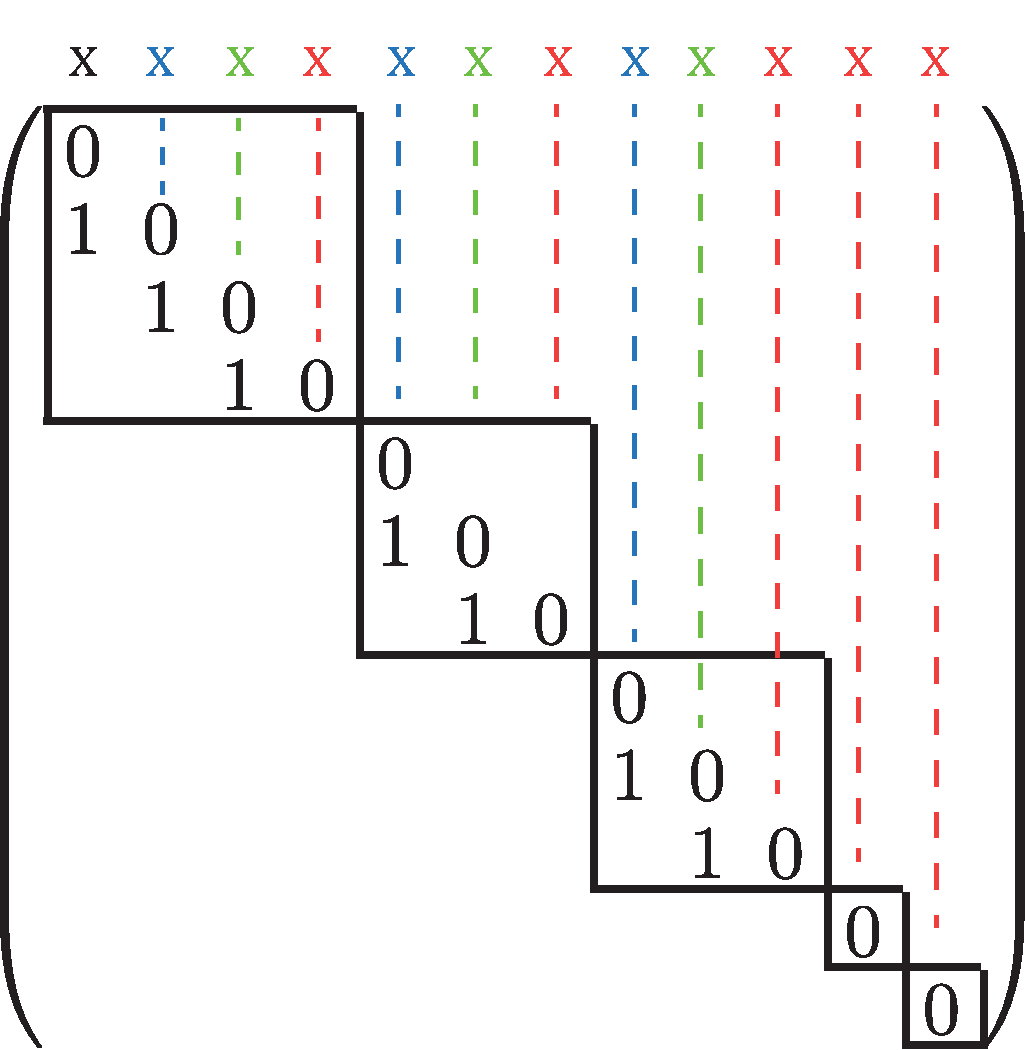
\includegraphics[scale=0.3]{Bilder/Kap6Ende.pdf}}}$
	\qquad \begin{minipage}[c]{7cm}
		\begin{align*}
			\Kern f &= \text{Eigenraum zum Eigenwert }0 \\
			&= \langle {\color{Firebrick2} x x x x x} \rangle \\
			\Kern f^2 &= \langle {\color{Chartreuse3} x x x}{\color{Firebrick2} x x x x x} \rangle\\
			\Kern f^3 &= \langle {\color{DodgerBlue3} x x x }{\color{Chartreuse3} x x x}{\color{Firebrick2} x x x x x} \rangle \\
			\Kern f^4 &= \langle  x {\color{DodgerBlue3} x x x }{\color{Chartreuse3} x x x}{\color{Firebrick2} x x x x x} \rangle 
		\end{align*}
	\end{minipage}
	}
\end{figure}
% subsection 624 (end)
% section 6 (end)
\newpage

\section{Die Jordansche Normalform} % (fold)
\label{sec:7}
\subsection[Bemerkung und Definition verallgemeinerte Eigenraum]{Bemerkung} % (fold)
\label{sub:71}
Sei $f \in \End(V)$ und $\lambda \in K$ ein Eigenwert von $f$. Für $t \in \mathds{N}$ sei $V^t (\lambda ) := \Kern (f- \lambda \id)^t $. Dann ist 
\[
	0 = V^0(\lambda ) \subseteq V^1 (\lambda ) \subseteq V^2(\lambda ) \subseteq V^3 (\lambda ) \subseteq \ldots 
\]
\[
	W_\lambda := \bigcup_{t=0}^\infty V^t (\lambda )
\]
heißt der \Index{verallgemeinerte Eigenraum} von $f$ zum Eigenwert $\lambda$. Ist $\dim V < \infty$, so gibt es ein minimales $k\ge 1$ mit $V^l(\lambda )= V^k(\lambda) $
für alle $l \ge k$. Dann $W_\lambda = V^k (\lambda )$.
% subsection 71 (end)

\subsection[Lemma: $\lambda $ ist der einzige Eigenwert von $f|_{W_\lambda}$]{Lemma} % (fold)
\label{sub:72}
$W_\lambda $ ist $f$-invariant. $\lambda $ ist der einzige Eigenwert von $f|_{w_{\lambda}}$
\minisec{Beweis}
Da $(f- \lambda )\circ  f = f \circ ( f- \lambda )$ ist auch $(f- \lambda )^t \circ f = f \circ ( f- \lambda )^t$. Ist $v \in V^t(\lambda)$, so ist 
\[
	(f- \lambda )^t \big(f(v)\big) = f  \big(\underbrace{(f- \lambda )^t (v)}_{=0 \text{ da } v \in V^t(\lambda)} \big) = 0 \enspace \Longrightarrow f(v) \in V^t(\lambda)
\]
Es sind also sogar alle $V^t(\lambda )$ $f$-invariant. Sei nun $\mu$ ein Eigenwert von $f|_{W_\lambda }$, also $f(w)= \mu \cdot  w$ mit $w \in W_{\lambda}, w \not= 0$. Dann $(f- \lambda)(w)= (\mu - \lambda )\cdot w$ und damit $(f- \lambda )^t (w) = (\mu - \lambda )^t \cdot w$.
Da $w \in W_\lambda $ gibt es $k$ mit $(f- \lambda )^k (w) = 0$. Es folgt 
\[
	0 = (\mu - \lambda)^k (w) \stackrel{w \not= 0 }{\Longrightarrow}  (\mu - \lambda )^k =0 \Rightarrow \mu - \lambda = 0 \Rightarrow \mu = \lambda \bewende
\]
% subsection 72 (end)

\subsection[Satz über eine Basis des verallgemeinerten Eigenraumes]{Satz} % (fold)
\label{sub:73}
Sei $f \in \End(V)$, $\dim V < \infty$, $\lambda $ ein Eigenwert von $f$. Sei $f_\lambda  := f|_{W_\lambda }$. Dann existiert eine Basis $B$ von $W_\lambda $ mit
\[
	m_B^B(f_\lambda ) = \left(\begin{BMAT}{ccc}{ccc}
		\JordLa{}  & & \\
		& \diagdown & \\
		& & \JordLa{}
	\end{BMAT} \right)
\]
\minisec{Beweis}
$g := (f_\lambda - \lambda )$ ist auf $W_\lambda $ nilpotent, da $W_\lambda = \Kern (f- \lambda )^k$ für ein geeignet großes $k$. Nach (\ref{sub:6215}) (i) gibt es eine
Basis $B$, so dass $m_B^B(g)$ die obige Form mit $\lambda =0$ hat.
Nun ist $m_B^B(f_\lambda )= m_B^B (g + \lambda )= m_B^B (g)+ m_B^B(\lambda ) = m_B^B (g)+ \lambda \cdot  I_n$ mit $n= \dim W_\lambda$. Also
\[
	m_B^B(f_\lambda) = \left(\begin{BMAT}{ccc}{ccc}
		\Jord  & & \\
		& \diagdown & \\
		& & \Jord
	\end{BMAT} \right) + \begin{pmatrix}
		\lambda & & \\
		 & \diagdown  & \\
		 & & \lambda 
	\end{pmatrix} = \left(\begin{BMAT}{ccc}{ccc}
		\JordLa{}  & & \\
		& \diagdown & \\
		& & \JordLa{}
	\end{BMAT} \right) \bewende
\]
% subsection 73 (end)

\subsection[Lemma über Teiler des charakteristischen Polynoms]{Lemma} % (fold)
\label{sub:74}
Sei $f \in \End(V)$, $\dim V < \infty$. Sei $\lambda $ ein Eigenwert von $f$. Dann teilt $(X- \lambda )^k$ genau dann das charakteristische Polynom $\chi_f$, wenn 
$k\le \dim W_\lambda$.
\minisec{Beweis}
Sei $F : \nicefrac{V}{W_\lambda } \to \nicefrac{V}{W_\lambda}$ von $f$ induziert. Nach (\ref{sub:611}) gilt: $\chi_f = \chi_{f|_{W_\lambda}} \cdot \chi_F$. Wegen
(\ref{sub:73}) ist $\chi_{f|_{W_\lambda }} = (X- \lambda )^n$ mit $n = \dim W_\lambda $. Insbesondere gilt $\chi_f = (X- \lambda )^n \cdot \chi_F$. 

Es bleibt zu zeigen: $(X- \lambda ) \nmid \chi_F$, also $\chi_F (\lambda  ) \not= 0$. Angenommen doch: $\chi_F (\lambda ) =0$. Dann ist $\lambda $ Eigenwert von $F$.
Sei $\overline{v} = v + W_{\lambda } \in \nicefrac{V}{W_\lambda }$ ein zugehöriger Eigenvektor. Also 
$f(v) + W_\lambda = F(\overline{v} ) = \lambda  \overline{v} = \lambda v + W_\lambda $. Also auch $w := f(v)- \lambda v \in W_\lambda $. Sei nun $k \in \mathds{N}$ mit
$(f- \lambda )^k (w') = 0 \, \forall w' \in W_\lambda  $. Insbesondere $(f- \lambda )^k (w) =0$. Dann ist 
\[
	(f- \lambda \id)^{k+1} (v) = (f- \lambda \id)^k (w) = 0 \qquad \text{ also } v \in W_\lambda 
\]
Es folgt $\overline{v} = v + W_\lambda = 0$ {\large $\lightning$} zu $\overline{v} $ ist Eigenvektor (also $\not=0$) \bewende
% subsection 74 (end)

\subsection[Lemma über den Schnitt von verallgemeinerten Eigenräumen]{Lemma} % (fold)
\label{sub:75}
Sei $f \in \End(V)$, $\dim V < \infty$. Sei $\Lambda$ die Menge der Eigenwerte von $f$. Für alle $\lambda  \in \Lambda$ gilt dann:
\[
	W_\lambda  \cap \sum_{\substack{\mu \in \Lambda \\ \mu \not= \lambda}} W_\mu = 0 
\]
\minisec{Beweis}
Wähle $n_\mu$ mit $W_\mu = \Kern (f- \mu)^{n_\mu}$. Da $(X- \lambda )^{n_\lambda }$ und $\prod_{\mu \not= \lambda , \mu \in \Lambda} (X- \mu)^{n_\mu}$
teilerfremd sind, gibt es Polynome $p_1, p_2 \in K[X]$ mit 
\[
	1 = p_1 \cdot (X- \lambda )^{n_\lambda } + p_2 \prod_{\substack{\mu \not= \lambda \\ \mu \in \Lambda}} (X- \mu)^{n_\mu} \tag{nach \ref{sub:413}\ref{413:enum:c}}
\]
Es folgt (durch Einsetzen von $f$).
\[
	\id = \underbrace{p_1(f) \circ (f- \lambda \id )^{n_\lambda }}_{=: f_1} + \underbrace{p_2 (f) \circ  \prod_{\substack{\mu \not= \lambda , \mu \in \Lambda}} (f- \mu \id)^{n_\mu}}_{=: f_2}
\]
Es ist $f_1 (w) =0 \, \forall w \in W_\lambda = \Kern (f- \lambda )^{n_\lambda }$. Da $(f- \mu)(f- \mu')= (f- \mu')(f- \mu)$ gilt $f_2 (w) = 0$ für alle 
$w \in \sum_{\mu \not=\lambda , \mu \in \Lambda} W_\mu  $. Es folgt $W_\lambda  \cap \sum_{\mu \not= \lambda} W_\mu = 0 $, da $f_1 + f_2 = \id$. \bewende
% subsection 75 (end)

\subsection[Satz über Summe der verallg. Eigenräume und $\chi_f$, wenn dies in Linearfaktoren zerfällt]{Satz} % (fold)
\label{sub:76}
Sei $f \in \End(V)$, $\dim V < \infty$. Sei $\Lambda$ die Menge der Eigenwerte von $f$. Weiter zerfalle $\chi_f$ in Linearfaktoren. Dann gilt
\[
	V = \bigoplus_{\lambda  \in \Lambda } W_\lambda \enspace, \enspace \chi_f = \prod_{\lambda \in \Lambda} (X-\lambda )^{n_\lambda } 
	\qquad \text{mit } n_\lambda  = \dim W_\lambda 
\]
\minisec{Beweis}
Es ist $\chi_f = \prod_{\lambda \in \Lambda} (X-\lambda )^{m_\lambda }$ für geeignete $m_\lambda  \ge 1$. Wegen (\ref{sub:74}) ist 
$m_\lambda  = n_\lambda = \dim W_\lambda $. Wegen (\ref{sub:75}) ist $\sum_{\lambda \in \Lambda} W_\lambda  = \bigoplus_{\lambda  \in \Lambda} W_\lambda  $. Da 
\[
	\dim V = d(\chi_f)=  \sum_{\lambda \in \Lambda} n_\lambda  = \dim \bigoplus_{\lambda \in \Lambda} W_\lambda 
\]
folgt $V= \bigoplus_{\lambda  \in \Lambda} W_\lambda $. \bewende 
% subsection 76 (end)

\subsection{Jordansche Normalform} % (fold)
\label{sub:77}
Sei $f \in \End(V)$, $\dim V < \infty$. $\chi_f$ zerfalle in Linearfaktoren. Dann gibt es eine Basis $B$ von $V$ mit \index{Jordansche Normalform}
\[
	m_B^B(f) = \left( \begin{BMAT}{cccc}{cccc}
		\boxed{K_1} & & & \\
		& \boxed{K_2} & & \\
		& & \diagdown & \\
		& & & \boxed{K_r}
	\end{BMAT} \right)
\]
wobei jedes $K_i =  \JordLa[i] $ ein Jordankasten ist. Jeder Eigenwert taucht mindestens einmal als Eigenwert eines der $K_i$ auf.
\minisec{Beispiel}
\[
	A= \begin{pmatrix}
		2 & 1 & 0 \\
		0 & 2 & 0 \\
		0 & 4 & 2
	\end{pmatrix} \qquad \chi_A = \det_{K[X]} \begin{pmatrix}
		X-2 & -1 & 0 \\
		0 & X-2 & 0 \\
		0 & -4 & X-2
	\end{pmatrix} = (X-2)^3
\]
Mögliche Jordansche Normalform für $A$:
\[
	J_1 = \left(\begin{BMAT}{ccc}{ccc}
		2 & & \\
		1 & 2 & \\
		& 1 &2
		\addpath{(0,0,:)rrruuulllddd}
	\end{BMAT}\right) \quad J_2 = \left(\begin{BMAT}{ccc}{ccc}
		2 & & \\
		1 & 2 & \\
		&  &2
		\addpath{(0,1,:)rruulldd}
		\addpath{(2,0,:)ruld}
	\end{BMAT} \right)\quad J_3 = \left(\begin{BMAT}{ccc}{ccc}
		2 & & \\
		 & 2 & \\
		&  &2
		\addpath{(0,2,:)ruld}
		\addpath{(1,1,:)ruld}
		\addpath{(2,0,:)ruld}
	\end{BMAT}\right)
\]
Eigenraum von $J_1$ zum Eigenwert 2 hat die Dimension: $\dim \Kern (2 I_3 - J_1)=  \dim \Kern \left(\begin{smallmatrix}
	0 & & \\
	-1 & 0 & \\
	 & -1 & 0 
\end{smallmatrix}\right) = 1$ \\
Eigenraum von $J_2$ zum Eigenwert 2 hat die Dimension: $\dim \Kern (2 I_3 - J_2)= \dim \Kern \left(\begin{smallmatrix}
	0 & & \\
	-1 & 0 & \\
	 &  & 0 
\end{smallmatrix}\right) = 2$ \\
Also ist $J_2$ die Jordansche Normalform von $A$.
\minisec{Frage}
Seien $A,B \in K^{n \times n}$ mit $\chi_A = \chi_B$ $\forall$ Eigenwerte $\lambda $ ist  $\dim V_\lambda (A) = \dim V_\lambda(B) $. Sind dann $A$ und $B$ konjugiert?
(bzw. sind die Jordanschen Normalformen gleich)\\
\uline{Nein!} Betrachte $A= \left( \begin{BMAT}{cccc}{cccc}
	2 & & & \\
	1 & 2 & & \\
	&  & 2 & \\
	& & 1& 2
	\addpath{(0,4,:)rrddlluu}
	\addpath{(2,2,:)rrddlluu}
\end{BMAT}\right)$ und $B= \left(\begin{BMAT}{cccc}{cccc}
	2 & & & \\
	1 & 2 & &  \\
	& 1& 2 & \\
	& &  & 2
	\addpath{(0,4,:)rrrdddllluuu}
	\addpath{(3,1,:)rdlu}
\end{BMAT}\right)$  Es gilt
\begin{align*}
	(B- 2 \cdot  I_4)^2  = \left( \begin{BMAT}{cccc}{cccc}
		0 & 0 & 0 & \\
		0 & 0 & 0 & \\
		1 & 0 & 0 & \\ 
		& & & 0
		\addpath{(0,4,:)rrrdddllluuu}
		\addpath{(3,1,:)rdlu}
	\end{BMAT} \right) \not= 0 \qquad \text{ aber } \qquad 
	(A- 2 \cdot I_4)^2 = \left( \begin{BMAT}{cccc}{cccc}
		0 & & & \\
		1 & 0 & & \\
		& & 0 & \\
		& & 1 & 0
		\addpath{(0,4,:)rrddlluu}
		\addpath{(2,2,:)rrddlluu}
	\end{BMAT} \right)^2 = 0
\end{align*}
% subsection 77 (end)

\subsection[Proposition: Binomischer Lehrsatz für Endomorphismen]{Proposition} % (fold)
\label{sub:78}
Seien $f,g  \in \End(V)$ mit $fg=gf$. Dann gilt 
\[
	(f+g)^n = \sum_{k=0}^{n} \binom{n}{k} f^k g^{n-k}
\]
\minisec{Beweis}
Für die Binomialkoeffizienten 
\[
	\binom{n}{k}= \begin{cases}
		\frac{n!}{k! (n-k)!} , &\text{ falls }0 \le k \le n\\
		0 , &\text{ sonst}
	\end{cases}
\]
gilt $\binom{n+1}{k}= \binom{n}{k} + \binom{n}{k-1}$. Die Aussage folgt per Induktion:
\begin{align*}
	(f+g)^{n+1} = (f+g) + (f+g)^n &= (f+g) \sum_{k=0}^{n} \binom{n}{k} f^k g^{n-k} \\
	&= \sum_{k=0}^{n}  \binom{n}{k} f^{k+1} g^{n-k} + \sum_{k=0}^{n} \binom{n}{k} f^k g{n-k+1} \\
	&= \sum_{k=0}^{n+1} \binom{n}{k-1} f^k g^{n+1-k} + \sum_{k=0}^{n} \binom{n}{k} f^k g^{n+1-k} \\
	&= \sum_{k=0}^{n+1} \enbrace*{ \binom{n}{k-1} + \binom{n}{k}} f^k g^{n+1-k} \\
	&= \sum_{k=0}^{n+1} \binom{n+1}{k} f^k g^{n+1-k} \bewende 
\end{align*}
% subsection 78 (end)

\subsection{Jordan-Chevalley-Zerlegung} % (fold)
\label{sub:79}
Sei $f \in \End(V), \dim V < \infty$, $\chi_f$ zerfalle in Linearfaktoren. Dann gibt es eine eindeutige Zerlegung $f= h+n$ mit 
\begin{enumerate}[1)]
	\item $h$ ist diagonalisierbar
	\item $n$ ist nilpotent
	\item $h n= n h$
\end{enumerate}
\minisec{Beweis}
\begin{description}
	\item[Existenz:] folgt aus (\ref{sub:77})
	\item[Eindeutigkeit:] Behauptung: Für $\lambda \in K$ gilt $(\star) \enspace W_\lambda (f) = V_\lambda (h)$. Sei $v \in V_\lambda (h)$, also $h(v)= \lambda v$.
	Dann gilt:
	\[
		(h+n-\lambda )^N (v) = \big(n+ (h-\lambda )\big)^N (v) = \sum_{k=0}^{N} \binom{N}{k} n^k (h-\lambda )^{N-k} (v) \stackrel{h(v)=\lambda v}{=} n^N \cdot (h-\lambda )^0 (v) = n^N (v)
	\]
	Da $n$ nilpotent ist, gibt es ein $N$ mit $n^N=0$. Es folgt $(f- \lambda )^N (v)= (h+n- \lambda )^N (v)= 0$ für dieses $N$. Also $v \in W_\lambda (f)$. Da 
	\[
		\bigoplus_{\lambda \in \Lambda} W_\lambda (f) = V \stackrel[{h \text{ diagonalisierbar}}]{}{=} \bigoplus_{\lambda  \in \Lambda}V_\lambda (h)  
	\]
	folgt nun aus $V_\lambda (h) \subseteq W_\lambda (f)$ schon $V_\lambda (h)= W_\lambda (f)$. Sei nun $f= h' + n'$ eine zweite Zerlegung mit 1)-3). Dann 
	\[
		V_\lambda (h) = W_\lambda (f) =V_\lambda (h') \quad \text{ wegen } (\star) 
	\]
	Da $h$ und $h'$ diagonalisierbar sind, folgt $h=h'$. Dann folgt auch $n=f-h=f-h'=n'$. \bewende
\end{description}
% subsection 79 (end)

\subsection[Definition: unipotenter Endomorphismus]{Definition} % (fold)
\label{sub:710}
Ein Endomorphismus der Form $f= \id +n$ mit $n$ nilpotent heißt \Index{unipotent}. 
% subsection 710 (end)

\subsection[Bemerkung über unipotente Endomorphismen]{Bemerkung} % (fold)
\label{sub:711}
Ist $f= \id + n$ unipotent mit $n^N=0$, so ist $f$ invertierbar mit 
\[
	f ^{-1} = \id - n + n^2 - n^3 + \ldots = \sum_{k=0}^{\infty} (-n)^k = \sum_{k=0}^{N-1} (-n)^k 
\]
% subsection 711 (end)

\subsection{Multiplikative Jordan-Chevalley-Zerlegung} % (fold)
\label{sub:712}
Sei $f \in GL(V), \dim V < \infty$, $\chi_f$ zerfalle in Linearfaktoren. Dann gibt es eine eindeutige Faktorisierung $f = h \cdot u$ mit
\begin{enumerate}[1)]
	\item $h$ ist diagonalisierbar
	\item $u$ ist unipotent
	\item $h \cdot u = u \cdot h$
\end{enumerate}
\minisec{Beweis}
Sind $h,n$ wie in (\ref{sub:79}) so erfüllt $(h, u = \id +n)$ 1) - 3) aus (\ref{sub:712}). Erfülle $h,u$ 1) - 3) aus (\ref{sub:712}) so erfüllen $(h, u- \id)$ 1) - 3) aus (\ref{sub:79}).
% subsection 712 (end)
% section 7 (end)
\newpage
\section{Das Minimalpolynom} % (fold)
\label{sec:8}

\subsection[Erinnerung an zyklische Unterräume]{Erinnerung} % (fold)
\label{sub:81}
Sei $f \in \End(V)$ zyklisch mit $V=L(v,f)$. Ist $n =\dim V$ so ist $B= \big(v, f(v),  \ldots, f^{n-1}(v) \big)$ eine Basis von $V$ und ist 
$f^n(v) = \sum_{i=0}^{n-1} \lambda_i f^i (v)$ so ist $\chi_f = X^n - \lambda_{n-1} X^{n-1} - \ldots  - \lambda_0$. (vergleiche \ref{sub:614})
% subsection 81 (end)

\subsection[Lemma über Gestalt von $\chi_f$ in \ref{sub:81}]{Lemma} % (fold)
\label{sub:82}
In der Situation von (\ref{sub:81}) gilt: $\chi_f (f) (v) =0$
\minisec{Beweis}
\[
	\chi_f (f) (v) = f^n (v) - \lambda_{n-1} f^{n-1}(v) - \ldots - \lambda_0 f^0(v) = 0 \bewende
\]
% subsection 82 (end)

\subsection{Satz von Cayley-Hamilton} % (fold)
\label{sub:83}
Sei $f \in \End(V)$, $\dim V < \infty$. Dann ist $\chi_f (f)=0$
\minisec{Beweis}
Sei $v \in V$. Sei $f_0$ die Einschränkung von $f$ auf den $f$-invarianten Unterraum $U:= L(v,f)$. Dann ist $\chi_{f_0} (f) v = \chi_{f_0} (f_0)=0$ wegen (\ref{sub:82}).
Sei $F : \nicefrac{V}{U} \to \nicefrac{V}{U}$ von $f$ induziert. Dann $\chi_f = \chi_{f_0} \cdot \chi_F = \chi_F \cdot \chi_{f_0}$. Es folgt
\[
	\chi_f (f) (v) = \Big(\chi_F (f)  \cdot \chi_{f_0}(f) \Big) (v) = \chi_F (f) \cdot  \Big(\chi_{f_0} (f)  (v) \Big) = 0  
\]
Also $\chi_f (f) (v) =0$ für alle $v \in V$. \bewende
% subsection 83 (end)

\subsection[Satz über Eigenschaften des Minimalpolynoms]{Satz} % (fold)
\label{sub:84}
Sei $f \in \End(V)$, $\dim V < \infty$. Dann gibt es ein eindeutiges normiertes Polynom $p \in K[X]$ minimalen Grades mit $p(f)=0$. Es gilt $p \mid \chi_f$.
\minisec{Beweis}
\begin{description}
	\item[Existenz:] folgt aus \hyperref[sub:83]{Cayley-Hamilton}
	\item[Eindeutigkeit:] Ist $q \in K[X]$ ein zweites normiertes Polynom mit $q(f)=0$. Ist $d(p)=d(q)$, so ist $d(p-q)< d(p) = d(q)$. Da $(p-q)(f)=0$ ist, folgt
	$p-q=0$ wegen der Minimalität von $d(p)$.  
	
	Division mit Rest liefert $\chi_f = l \cdot p +r$ mit $d(r)< d(p)$. Da $r(f)= \chi_f (f) - l(f) p(f)=0$ ist folgt mit der Minimalität von $d(p)$ wieder $r=0$.\bewende 
\end{description}
% subsection 84 (end)

\subsection[Definition Minimalpolynom]{Definition} % (fold)
\label{sub:85}
$p$ aus (\ref{sub:84}) heißt das \Index{Minimalpolynom} von $f$. Wir bezeichnen es mit $p_f$. 
% subsection 85 (end)

\subsection[Lemma: Nullstellen von $p_f$ sind Eigenwerte von $chi_f$]{Lemma} % (fold)
\label{sub:86}
$p_f (\lambda ) = 0 \iff \lambda $ ist Eigenwert von $f$.
\minisec{Beweis}
Ist $\lambda $ eine Nullstelle von $p_f$ so ist $\lambda $ auch eine Nullstelle von $\chi_f$ (da $p_f \mid \chi_f$) und damit ein Eigenwert von $f$. Ist umgekehrt $\lambda $
ein Eigenwert von $f$ mit Eigenvektor $v$, so folgt mit $p_f = a_n X^n + a_{n-1} X^{n-1} + \ldots + a_0$
\[
	0 = p_f(f)  (v) = \sum_{k=0}^{n} a_k f^k(v) = \sum_{k=0}^{n} a_k \lambda^k \cdot v = p_f (\lambda ) \cdot v 
\]
Da $v \not= 0$ ist, folgt $p_f (\lambda ) =0$. \bewende
% subsection 86 (end)

\subsection[Lemma über das Minimalpolynom, wenn $f$ diagonalisierbar]{Lemma} % (fold)
\label{sub:87}
Ist $f$ diagonalisierbar, so ist 
\[
	p_f = \prod_{\lambda \text{ Eigenwert von }f} (X- \lambda ) \tag{$\star$}
\]
\minisec{Beweis}
Sei $q$ die rechte Seite von ($\star$). Wegen (\ref{sub:86}) teilt $q$ das Minimalpolynom $p_f$. Es bleibt zu zeigen $q(f)=0$. Sei $v$ ein Eigenvektor von $f$ zum 
Eigenwert $\lambda $. Schreibe $q=q_0 (X -\lambda )$. Dann 
\[
	q(f) (v) = q_0 (f) \big(\underbrace{(f- \lambda) (v)}_{=0} \big) =0 
\]
Da $f$ diagonalisierbar ist, gibt es eine Basis von $V$ aus Eigenvektoren von $f$. Nun wirkt $q(f)$ trivial auf dieser Basis. Damit  folgt $q(f)=0$. \bewende
% subsection 87 (end)

\subsection[Lemma: $p_f$ ist Produkt von verschiedenen Linearfaktoren $\Rightarrow f$ ist diagonalisierbar]{Lemma} % (fold)
\label{sub:88}
Sei $f \in \End(V)$, $\dim V < \infty$. Weiter sei $p_f = (X- \lambda_1) \cdot  \ldots \cdot (X- \lambda_n)$ das Produkt von paarweise verschiedenen Linearfaktoren. Dann
ist $f$ diagonalisierbar.
\minisec{Beweis}
Mit Division mit Rest erhalten wir mit einem festen $i$
\[
	\prod_{j \not= i} (X- \lambda_j) = q_i \cdot (X- \lambda_i) + c_i \tag*{$c_i  \in K, q_i \in K[X]$}
\]
da die $\lambda_j$ paarweise verschieden sind, ist $c_i \not=0$. Es folgt für $v \in V$
\[
	c_i  v = \underbrace{\prod_{j \not= i} (f- \lambda_j) (v)}_{v_i} - \underbrace{(f- \lambda i) q_i (f) (v)}_{w_i}
\]
Es ist $v_i \in \Kern (f- \lambda_i)$, da $0=p_f(f) = \prod_j (f- \lambda_j)$. Weiter ist $w_i \in \bild (f- \lambda_i)$. Es gilt also
\begin{align*}
	V &= \Kern (f- \lambda_i) \oplus \bild (f- \lambda_i) \\
	&= V_{\lambda_i} \oplus \bild (f-\lambda_i) \tag{$\star$} 
\end{align*}
Sei $U:= \bigoplus_{i} V_{\lambda_i} \subseteq V$. Wegen ($\star$) ist die von $(f- \lambda_i)$ induzierte Abbildung auf $\nicefrac{V}{U}$ surjektiv. Also induziert auch 
$0= (f-\lambda_1) \cdot \ldots \cdot (f- \lambda_n)$ eine surjektive Abbildung auf $\nicefrac{V}{U}$. Es folgt $\nicefrac{V}{U}=\{0\}$. Also 
$V=U = \bigoplus_{i} V_{\lambda_i}$ und $f$ ist diagonalisierbar. \bewende
% subsection 88 (end)

\subsection[Satz: die Diagonalisierbarkeit von $f \iff$ Gestalt von $p_f$]{Satz} % (fold)
\label{sub:89}
Sei $f \in \End(V)$, $ \dim V < \infty$. Dann ist $f$ genau dann diagonalisierbar, wenn $p_f$ ein Produkt von paarweise verschiedenen Linearfaktoren ist.
\minisec{Beweis}
(\ref{sub:87}) und (\ref{sub:88})
% subsection 89 (end)

\subsection[Beispiel: Minimalpolynom eines Jordankastens]{Beispiel} % (fold)
\label{sub:810}
Sei $J= \JordLa$ ein Jordankasten der Größe $n$. Dann gilt $p_J = (X-\lambda )^n$
\minisec{Beweis}
Es ist $\chi_J = (X-\lambda )^n$. Da $p_J \mid \chi_J$ ist $p_J = (X-\lambda )^k$ mit $k \le n$. Da $(J-\lambda )= \Jord$ ist leicht zu sehen, dass $(J-\lambda )^k \not= 0$ für $k <n$. Es folgt $p_J=(X-\lambda )^n$. \bewende
% subsection 810 (end)

\subsection[Satz über die Gestalt von $p_f$, hergeleitet aus der JNF]{Satz} % (fold)
\label{sub:811}
Sei 
\[
	A = \begin{pmatrix}
		\boxed{J_1} & & \\
		& \ddots & \\
		& & \boxed{J_n}
	\end{pmatrix}
\]
wobei jedes $J_i$ ein Jordankasten mit $\lambda_i$ auf der Diagonalen ist. Für jeden Eigenwert $\lambda$ von $A$ sei $n_\lambda $ die Größe des größten Jordankasten zum 
Eigenwert $\lambda $. Dann gilt: 
\[
	p_A = \prod_{\lambda \text{ EW}} (X- \lambda )^{n_\lambda }
\]
\minisec{Beweis}
Folgt mit (\ref{sub:810}) \bewende
% subsection 811 (end)

\subsection[Lemma über Vertäglichkeit von $m_B^B$ mit dem Minimalpolynom]{Lemma} % (fold)
\label{sub:812}
Sei $p \in K[X]$ und $B$ eine endliche Basis von $V$. Für $f \in \End(V)$ gilt $p \enbrace*{m_B^B(f)} = m_B^B \big( p(f) \big) $
\minisec{Beweis}
$m_B^B : \End(V) \to K^{n \times n}$ ist linear und verträglich mit Komposition. Ist $p= \sum_{k=0}^{n}  a_k X^k$ so folgt:
\[
	p\big( m_B^B(f)\big) = \sum_{k=0}^{n} a_k \big( m_B^B (f) \big)^k = \sum_{k=0}^{n} a_k \cdot m_B^B(f^k) = m_B^B \left( \sum_{k=0}^{n} a_k f^k \right) = m_B^B \big( p(f) \big) 
	\bewende
\]
% subsection 812 (end)

\subsection[Korollar über Gleichheit der Minimalpolynome von $f$ und $m_B^B(f)$]{Korollar} % (fold)
\label{sub:813}
$p_f = p_{m_B^B (f)}$
\minisec{Beweis}
(\ref{sub:812}) \bewende
% subsection 813 (end)

\subsection[Bemerkung: Die Einsetzungshomomorphismen und $m_B^B$ sind Ringhomomorphismen]{Bemerkung} % (fold)
\label{sub:814}
Zu $f \in \End(V), A \in K^{n \times n}$ sind die Einsetzungshomomorphismen
\begin{align*}
	\Phi_f &: K[X] \to \End(V) \enspace, \Phi_f (p) := p(f) \\
	\Phi_A &: K[X] \to K^{n \times n} \enspace, \Phi_A (p) := p(A) \\
\end{align*}
Ringhomomorphismen. Ebenso ist $m_B^B : \End(V) \to K^{n \times n}$ ein \Index{Ringhomomorphismus}. Nach (\ref{sub:812}) kommutiert das Diagramm
\[
	\begin{tikzcd}
		K[X] \rar{\Phi_f} \arrow[bend right, swap]{dr}{\Phi_{m^B_B(f)}}& \End(V)  \dar{m^B_B}\\
		  & K^{n \times n}
	\end{tikzcd}
\]
% subsection 814 (end)

\subsection[Bemerkung über Bilder der Einsetzungshomomorphismen]{Bemerkung} % (fold)
\label{sub:815}
$\bild ( \Phi_f) \subseteq \End(V)$ und $\bild (\Phi_A) \subseteq K^{n \times n}$ sind kommutative Unterringe von $\End(V)$ bzw. $K^{n \times n}$
% subsection 815 (end)

\subsection[Satz: Beweis des Kochrezepts für die Jordan-Normalform]{Satz} % (fold)
\label{sub:816}
Sei $f \in \End(V)$, $\dim V < \infty$. Das charakteristische Polynom $\chi_f$ zerfalle in Linearfaktoren. Sei $\Lambda$ die Menge der Eigenwerte von $f$. Für 
$\lambda \in \Lambda$ sei $d_{\lambda,k} := \dim \Kern (f-\lambda )^k$ und $d_{\lambda, 0} := 0$. Sei $j_{\lambda, k}$ die Anzahl der $k \times k$ Jordankästen zum Eigenwert $\lambda$. Dann gilt:
\[
	j_{\lambda,k} = 2 \cdot d_{\lambda, k} - \enbrace*{ d_{\lambda, k+1} + d_{\lambda, k-1}}
\]
\minisec{Beweis}
Sei $J= \left( \begin{smallmatrix}
	\boxed{J_1} & & \\
	& \diagdown & \\
	& & \boxed{J_n}
\end{smallmatrix} \right)$ die Jordan-Normalform zu $f$. Dann gilt
\[
	(J - \lambda )^k = \begin{pmatrix}
		(J_1-\lambda )^k & & \\
		& \diagdown & \\
		& & (J_n - \lambda )^k
	\end{pmatrix}
\]
Also ist $d_{\lambda, k} = \sum_{i=1}^{n} \dim \Kern (J_i - \lambda )^k$. Ist $J_i$ ein $l \times l$ Jordankasten zum Eigenwert $\mu$, so gilt
\[
	\dim \Kern (J_i - \lambda )^k = \begin{cases}
		0, &\text{ falls }\lambda  \not= \mu\\
		\min \set{k,l} , &\text{ falls } \lambda = \mu 
	\end{cases}
\]
Es folgt: 
\begin{align*}
	d_{\lambda,1} &= \sum_{l=1}^{\dim V} j_{\lambda,l} \\
	d_{\lambda ,2} &= \sum_{l=1}^{\dim V} j_{\lambda , l} + \sum_{l=2}^{\dim V} j_{\lambda,l} \\
	\ldots & \\
	d_{\lambda, k} &= d_{\lambda, k-1} + \sum_{l=k}^{\dim V} j_{\lambda,l} \Longrightarrow  d_{\lambda,k} - d_{\lambda, k-1} = \sum_{l=k}^{\dim V} j_{\lambda, l}
\end{align*}
Also ist 
\begin{align*}
	2 \cdot d_{\lambda ,k} - (d_{\lambda, k+1} + d_{\lambda, k-1}) = (d_{\lambda , k} - d_{\lambda , k-1}) - (d_{\lambda, k+1} - d_{\lambda,k}) = 
	\sum_{l=k}^{\dim V} j_{\lambda, l} - \sum_{l=k+1}^{\dim V} j_{\lambda, l} = j_{\lambda , k} \bewende  
\end{align*}
% subsection 816 (end)
% section 8 (end)
\newpage
\section{Euklidische Ringe und Hauptidealringe} % (fold)
\label{sec:9}
\subsection[Definiton Ideal]{Definition} % (fold)
\label{sub:91}
Sei $R$ ein kommutativer Ring. Eine Teilmenge $I \subset R$ heißt \Index{Ideal} falls gilt: 
\begin{enumerate}[i)]
	\item $I \subseteq R$ ist eine Untergruppe bezüglich $+$
	\item $\forall a \in I, \forall r \in R : r \cdot a \in I$
\end{enumerate}
% subsection 91 (end)

\subsection[Beispiele für Ideale]{Beispiele} % (fold)
\label{sub:92}
\begin{enumerate}[i)]
	\item $I=R$, $I= \set{0} \subseteq R $
	\item Sei $R=\mathds{Z}$, $2 \mathds{Z} = \set[2 n]{n \in \mathds{Z}} \subseteq \mathds{Z} $ ist ein Ideal
	\item Sei $R=\mathds{Z}$, $n$ fest. $n \mathds{Z} = \set[n \cdot z]{z \in \mathds{Z}} \subseteq \mathds{Z} $ ist ein Ideal
	\item $I= \set[\sum_{k=1}^{n} a_k X^k]{a_k \in 2 \mathds{Z}} \subseteq \mathds{Z}[X] $ ist ein Ideal
\end{enumerate}
% subsection 92 (end)

\subsection[Definition Einheit]{Definition} % (fold)
\label{sub:93}
$u \in R$ heißt \Index{Einheit}, falls es ein $r \in R$ gibt, so dass $u \cdot r = 1$. Die Einheiten eines Ringes bilden eine Gruppe $R^\times$. 
% subsection 93 (end)

\subsection[Lemma über Ideale und Einheiten]{Lemma} % (fold)
\label{sub:94}
Sei $I \subset R$ ein Ideal. Dann sind äquivalent:
\begin{enumerate}[(i)]
	\item $I = R$
	\item $1 \in I$
	\item $I$ enthält eine Einheit
\end{enumerate}
\minisec{Beweis}
\begin{description}
	\item[(i)$\Rightarrow$(ii)] klar
	\item[(ii)$\Rightarrow $(iii)] klar
	\item[(iii)$\Rightarrow $(i)] $I \subseteq R$ per Definition. Also nu $R \subseteq I$ zu zeigen: \\
	Sei $r \in R$ und $u$ die Einheit in $I$. Dann ist $r= (r \cdot u ^{-1}) \cdot u \in I$ \bewende
\end{description}
% subsection 94 (end)

\subsection[Bemerkung über die Ideale eines Körpers]{Bemerkung} % (fold)
\label{sub:95}
$\set{0} $ und $K$ sind die einzigen Ideale des Körpers $K$.
% subsection 95 (end)

\subsection[Definition: kleinstes und erzeugtes Ideal]{Definition} % (fold)
\label{sub:96}
Seien $a_1, \ldots , a_n \in R$. Mit $(a_1, \ldots , a_n)$ bezeichnen wir das kleinste Ideal \index{Ideal!kleinstes} von $R$, das $a_1, \ldots , a_n$ enthält. Also 
\[
	(a_1, \ldots , a_n) := \bigcap_{I \subset R, a_1, \ldots , a_n \in I} I
\]
$(a_1, \ldots , a_n)$ heißt das von $a_1, \ldots , a_n$ erzeugte Ideal. \index{Ideal!erzeugtes}
\minisec{Bemerkung}
\[
	(a_1, \ldots , a_n) = \set[\sum_{i=1}^{n} r_i a_i]{r_i \in R} 
\]
% subsection 96 (end)

\subsection[Definition: Hauptideal]{Definition} % (fold)
\label{sub:97}
Ideale, die von einem Element erzeugt werden, heißen \Index{Hauptideale} 
% subsection 97 (end)

\subsection[Definition Integritätsring und Hauptidealring]{Definition} % (fold)
\label{sub:98}
Ein \Index{Integritätsring} $R$ ist ein kommutativer nullteilerfreier Ring. Ein Integritätsring heißt \Index{Hauptidealring} (HIR), wenn alle Ideale Hauptideale sind.  
\minisec{Beispiel}
Jeder Körper ist ein Hauptidealring.
% subsection 98 (end)

\subsection[Definition: Euklidischer Ring und Gradfunktion]{Definiton} % (fold)
\label{sub:99}
Ein Integritätsring heißt \Index{euklidscher Ring}, wenn es eine Abbildung $\delta : R \setminus \{0\} \to \mathds{N}$ mit folgenden Eigenschaften gibt 
$\forall a,b \in R, b \not= 0 \enspace\exists q,r \in R : a= qb +r , \delta (r) < \delta (b)$ oder $r =0$.
$\delta $ heißt dann eine \Index{Gradfunktion} 
% subsection 99 (end)

\subsection[Beispiel für euklidische Ringe]{Beispiel} % (fold)
\label{sub:910}
\begin{enumerate}[(i)]
	\item $\mathds{Z}$ ist ein euklidscher Ring ($\delta (n) := \abs{n} $)
	\item $K[X]$ ist ein euklidscher Ring ($\delta (p) := d(p)$ vgl. \ref{sub:47}) 
\end{enumerate}
% subsection 910 (end)

\subsection[Satz: Euklidische Ringe sind Hauptidealringe]{Satz} % (fold)
\label{sub:911}
Euklidsche Ringe sind Hauptidealringe.
\minisec{Beweis}
Sei $I \subseteq R$ ein Ideal. Ist $I= \{0\}$, so ist nichts mehr zu tun. Sei also $\{0\} \not= I$. Wähle $b \in I \setminus \{0\}$ so, dass $\delta (b)$ minimal ist.
Behauptung: $I= (b)$ 
\begin{description}
	\item[\glqq$\subseteq$\grqq] Sei $a \in I$. Dann ist $a = qb +r$ mit $r=0$ oder $\delta (r) < \delta (b)$. Da $r= a- qb \in I$ ist und $\delta (b)$ minimal war, folgt
	$\delta (r) \ge \delta (b)$ {\large $\lightning$}. Also $r=0$. Es folgt $a= q \cdot b$, also $a \in (b)$
	\item[\glqq$\supseteq $\grqq] klar, da $b \in I$ \bewende 
\end{description}
% subsection 911 (end)

\subsection[Definition von irreduzibel und prim in Integritätsringen]{Definition} % (fold)
\label{sub:912}
Sei $R$ ein Integritätsring. Sei $p \in R$, $p \not= 0, p \not\in R^\times$
\begin{enumerate}[(i)]
	\item $p$ heißt \Index{irreduzibel}, falls $p=a \cdot b \quad  a,b \in R \Rightarrow a \in R^\times$ oder $b \in R^\times$
	\item $p$ heißt \Index{prim}, falls : $p \mid a \cdot b  \quad  a,b \in R \Rightarrow p \mid a$ oder $p \mid b$ 
\end{enumerate}
% subsection 912 (end)

\subsection[Lemma: prim impliziert irreduzibel]{Lemma} % (fold)
\label{sub:913}
Ist $p$ prim, so ist $p$ irreduzibel
\minisec{Beweis}
Sei $p =a \cdot b$, $p$ prim $\Rightarrow p \mid a$ oder $p \mid b$. oBdA $p \mid a$. D.h. $\exists u \in R$, so dass $p \cdot u = a$. Daraus folgt $p=ab=pub \Leftrightarrow p - pub = 0$
$\Rightarrow p(1- ub) = 0 \xrightarrow{\text{nullteilerfrei}}  1- ub = 0$, also $ub = 1$. Also ist $b$ eine Einheit. \bewende
% subsection 913 (end)

\subsection[Satz: In Hauptidealringen ist prim äquivalent zu irreduzibel]{Satz} % (fold)
\label{sub:914}
Sei $R$ ein Hauptidealring. Dann gilt: $p$ ist prim $\iff$ $p$ irreduzibel
\minisec{Beweis}
\begin{description}
	\item[\glqq$\Rightarrow $\grqq:] \ref{sub:913}
	\item[\glqq$\Leftarrow $\grqq:] Sei $p$ irreduzibel. Seien $a,b \in R$ mit $p \mid a \cdot b$, $p \nmid a$. Zu zeigen: $p \mid b$.
	
	Dazu $R$ Hauptidealring, d.h. $\exists d \in R$ mit $(a,p)= (d)$. Also $\exists c \in R$ mit $p=c \cdot d$. Da $p$ irreduzibel ist, muss $c \in R^\times$ oder 
	$d \in R^\times$ gelten. Angenommen $c \in R^\times$. Dann ist $d= c ^{-1} p$. Wegen $a \in (d)$ gibt es nun $f \in R$ mit $a= f \cdot d \Rightarrow a = f c ^{-1} p \Rightarrow p \mid a $ {\large $\lightning$} zur Vorraussetzung. 
	
	Also muss $d \in R^\times$ gelten. Also $(d)= R= (a,p)$. Also gibt es $r,s \in R$ mit $1= ra + sp \Rightarrow b = rab + spb \Rightarrow p \mid b$ \bewende
\end{description}
% subsection 914 (end)

\subsection[Satz über die Existenz der Primfaktorzerlegung in Hauptidealringen]{Satz} % (fold)
\label{sub:915}
Sei $R$ ein Hauptidealring. Dann lässt sich jedes $a \in R$, $a \not= 0$, $a \not\in R^\times$ als ein Produkt von endlich vielen Primelementen aus $R$ schreiben.
\minisec{Beweis (mit \ref{sub:916})}
Wir nennen $a \in R, a \not= 0$, $a \not\in R^\times$ "gut", falls es das Produkt von endlich vielen Primelementen ist. Angenommen $a \in R \setminus \{0\} \cup R^\times$ 
ist nicht "gut". Dann ist $a$ nicht prim, also nach (\ref{sub:914}) auch nicht irreduzibel. Also $a= a_1 b_1$ für $a_1, b_1 \not\in R^\times$. Dann ist entweder $a_1$ nicht 
gut oder $b_1$. Sei o.B.d.A also $a_1$ nicht gut. $\leadsto$ Folge $a_1 a_2, \ldots , b_1 b_2, \ldots  \in R \setminus R^\times$ mit $a_i = a_{i+1} b_{i+1}$ ($a= a_0$).
Also $(a) \subseteq (a_1) \subseteq (a_2) \subseteq \ldots $. Wegen (\ref{sub:916}) $\exists N$ mit $(a_N) = (a_{N+1}) = (a_N b_N)$. Also $\exists u \in R$ mit 
$a_N = a_N b_N u$. Da $R$ nullteilerfrei ist folgt $b_N u = 1 \Rightarrow b_N \in R^\times$ {\large $\lightning$} \bewende
% subsection 915 (end)

\subsection[Lemma über eine aufsteigende Folge von Idealen]{Lemma} % (fold)
\label{sub:916}
Sei $R$ ein Hauptidealring. Sei $I_1 \subseteq I_2 \subseteq \ldots $ eine aufsteigende Folge von Idealen in $R$. Dann gibt es eine $N \in \mathds{N}$ so dass 
$I_n = I_N \forall n \ge N$.
\minisec{Beweis}
Definiere $I := \bigcup_{n=1}^\infty I_n$ ist ein Ideal. Also $\exists a \in R$ mit $I=(a)$. Sei $a \in I_N$. Es folgt 
\[
	I=(a) \subseteq I_N \subseteq I_n \subseteq  I_{n+1} \subseteq \ldots \subseteq I
\]
Also $I_N = I_n \forall n \ge N$. \bewende
% subsection 916 (end)

\subsection{Eindeutige Primfaktorzerlegung in Hauptidealringen} % (fold)
\label{sub:917}
Sei $R$ ein Hauptidealring. 
\begin{enumerate}[1)]
	\item Jedes $a \in R$, $a \not= 0$, $a \not\in R^\times$ ist das Produkt von endlich vielen Primelementen $a= p_1 \cdot  \ldots \cdot p_N$
	\item Ist $p_1 \cdot \ldots \cdot p_N = q_1 \cdot \ldots \cdot  q_M$ mit $p_i, q_j $ prim, so gilt $N=M$ und es gibt $u_1, \ldots , u_N \in R^\times$ so dass 
	(nach Umnummerierung) $p_i = q_i u_i$
\end{enumerate}
\minisec{Beweis}
\begin{enumerate}[1)]
	\item (\ref{sub:915})
	\item per Induktion nach $N$. \begin{description}
		\item[$N=1$] $\surd$
		\item[$N-1 \mapsto N$] \begin{itemize}
			\item Ist $p_1 \cdot  \ldots \cdot  p_N = q_1 \cdot \ldots \cdot q_M$ mit $p_i, q_i$ prim, so gilt insbesondere $p_1 \mid q_1 \cdot \ldots \cdot q_M$
			\item Da $p_1$ prim, folgt o.B.d.A. $p_1 \mid q_1 \Rightarrow c p_1 = q_1$.
			\item Da $q_1$ prim (und somit irreduzibel) ist, folgt $p_1 = u_1 q_1$ mit $u_1 \in R^\times$.
		\end{itemize} 
		Also ist 
		\[
			q_1 \cdots q_m = p_1 \cdots p_N = q_1 u_1 p_2 \cdots p_N \stackrel{R \text{ nullteilerfrei}}{\Longrightarrow} q_2 \cdots q_M = u_i p_2 \cdots p_M 
			\stackrel{\text{I.V.}}{\Rightarrow } \text{ Beh.} \bewende
		\]
	\end{description}
\end{enumerate}
% subsection 917 (end)

\subsection[Definition: Ring der Gaußsche Zahlen]{Definition} % (fold)
\label{sub:918}
Der Ring 
\[
	\mathds{Z}[i] := \set[a + bi]{a,b \in \mathds{Z}} \subset \mathds{C} 
\]
heißt Ring der \Index{Gaußschen Zahlen}.
% subsection 918 (end)

\subsection[Lemma: Der Ring der Gaußschen Zahlen ist ein Hauptidealring]{Lemma} % (fold)
\label{sub:919}
$\mathds{Z}[i]$ ist ein Euklidischer Ring (und damit ein Hauptidealring).
\minisec{Beweis}
\begin{itemize}
	\item $\mathds{Z}[i]$ ist Integritätsring, definiere $N : \mathds{Z}[i] \setminus \{0\} \to \mathds{N}$ mit $a+ ib \mapsto a^2 + b^2 = \abs{a+ ib}^2 $. Damit ist $N$
	multiplikativ. Sei nun $z, \zeta \in \mathds{Z}[i], \zeta \not= 0$. Zu zeigen: $\exists q,r \in \mathds{Z}[i]$ mit $z= q \zeta +r$ und $r=0$ oder 
	$N(r) < N(\zeta)$. Es gilt \begin{itemize}
		\item $\zeta \in \mathds{C}^\times \Rightarrow z \cdot \zeta ^{-1} \in \mathds{C}$
		\item Für benachbarte $f,g \in \mathds{Z}[i]$ ist $\abs{f-g} \le \sqrt{2}$
	\end{itemize}
	Also gibt es zu $h \in \mathds{C}$ eine Gaußsche Zahl $q$ mit $\abs{h-q} \le \frac{1}{\sqrt{2}} = \frac{1}{2} \sqrt{2}     $
	\item Wähle so ein $q \in \mathds{Z}[i]$ für $h = z \cdot \zeta ^{-1}$ und setze $r := z - q \cdot \zeta \in \mathds{Z}[i]$. Dann ist $z= q \cdot \zeta +r$ und 
	\[
		\abs{r} = \abs{z- q \zeta} = \abs{\zeta} \cdot \underbrace{\abs{z \zeta ^{-1} - q}}_{\le \frac{1}{\sqrt{2}} < 1} \le \abs{\zeta} \tag{$()^2$ für $N$}
	\]
	mit $\zeta \not= 0 $ folgt $ N(r) < N(\zeta)$ \bewende
\end{itemize}
% subsection 919 (end)

\subsection[Lemma: Einheiten in den Gaußschen Zahlen]{Lemma} % (fold)
\label{sub:920}
\begin{enumerate}[a)]
	\item $\mathds{Z}[i]^\times = \set{\pm 1, \pm i} $
	\item Ist $c \in \mathds{Z}[i]$ mit $N(c)= \abs{c}^2 = 1 $, so ist $c \in \mathds{Z}[i]^\times$
\end{enumerate}
\minisec{Beweis}
\begin{enumerate}[a)]
	\item \glqq$\supseteq$\grqq: klar \\
	\glqq$\subseteq$\grqq: Sei $u \in \mathds{Z}[i]^\times$. Dann ist $1=N(1)= N(u u ^{-1}) = N(u) \cdot N(u ^{-1})$. Dann ist $N(u) = 1$. Sei $u= a+ ib$, also 
	$1= a^2 + b^2 \Rightarrow $ Behauptung
	\item schon erledigt \bewende
\end{enumerate}
% subsection 920 (end)

\subsection[Satz: Lösung von $x^2 +1 = y^3$]{Satz} % (fold)
\label{sub:921}
Die einzige ganzzahlige Lösung der Gleichung $x^2 +1 = y^3$ ist $x=0, y= 1$.
\minisec{Beweis}
Seien $x,y \in \mathds{Z}$ mit $x^2 +1 = y^3$. Ist $x=0$ folgt $y=1$. Die Annahme $x=\pm 1$ führt zu $y^3 = 2$, was in $\mathds{Z}$ nicht lösbar ist. Also können wir 
$x \not\in \{0, \pm 1 \}$ annehmen. \begin{enumerate}[i)]
	\item Betrachte $y^3 = x^2 +1 = (x+i)(x-i)$ in $\mathds{Z}[i]$. Da $x \not= 0$ ist $x+1, x-1 \not\in \mathds{Z}[i]^\times$. (siehe \ref{sub:920})
	\item \label{921:Beh}Behauptung: Ist $c$ ein gemeinsamer Teiler von $x+i$ und $x-i$ ist, so ist $c$ bereits eine Einheit.
	
	Beweis: Ist $c \mid x+i \enspace\wedge \enspace c \mid x-i$, so ist auch $c \mid (x+i)- (x-i) = 2i$. Wegen $N(2i) = 4$, muss $N(c) \in \set{1,2,4}$ gelten. 
	\marginnote{$N$ multiplikativ}
	Ist $N(c) = 1$ so folgt mit (\ref{sub:920}) $c \in \mathds{Z}[i]^\times$. 
	\begin{table}[h]
		\centering{\begin{tabular}{c|cccc}
		$N(a+ b i)=a^2 + b^2$ & $1$ & $2$ & $3$ & $4$\\
		\midrule
		$a+ b i$ & $\pm 1, \pm i$ & $\pm 1+i, \pm 1-i$ & / & $\pm 2, \pm 2i$
		\end{tabular}
		\caption{Lösungen für $N(a+ bi) \in \set{1,2,3,4}$}}
	\end{table}
	Ist also $N(c)=4$, so ist $c = \pm 2$ oder $\pm 2i$, so folgt $c \nmid x+1$ in $\mathds{Z}[i]$. \light
	
	Ist $N(c)=2$ folgt $c \in \set{\pm 1 +i, \pm 1-i} \Rightarrow c= 1+i$ bis auf Muliplikation mit einer Einheit. Es folgt 
	\[
		1+i \mid (x+i)(x-i)= y^3 \stackrel{(\star)}{\Longrightarrow} 1+ i \mid y \Rightarrow (1+i)^3 \mid y^3 = (x+i)(x-i) \stackrel{\text{PFZ}}{=} (p_1 \cdots p_N)(q_1 \cdots q_M)
	\]
	zu $(\star)$: $1+i$ ist prim in $\mathds{Z}[i]$, da aus $1+i = z_1 z_2$ folgt $0=N(1+i)= N(z_1) \cdot N(z_2) \Rightarrow $ o.B.d.A $N(z_1)=1$ 
	also $z_1 \in \mathds{Z}[i]^\times$
	\[
		\Longrightarrow \quad (1+i)(1+i)(1+i) \cdot( r_1 + r_k) = (p_1 \cdots p_N)(q_1 \cdots q_M)
	\]
	Es folgt $(1+i)^2 = 2i \mid x+i$ oder $(1+i)^2  = 2i\mid (x-i) \Rightarrow  2 \mid x+i$ oder $2 \mid x-i$ \light
	
	Also kann $c$ nur noch eine Einheit sein.
	\item Die Primfaktorzerlegung liefert 
	\[
		y^3 = (t_1 \cdots t_L)^3 = t_1 t_1 t_1 \cdots t_2 t_2 t_2 = x^2 +1 = (x +i) (x-i)
	\]
	mit Behauptung \ref{921:Beh}) folgt nach Umnummerierung $(x+i)= t_1 ^3 \cdots t_{\nu} ^3$ und $x-i = t_{\nu +1} ^3 \cdots t_L^3$. Also existieren $a,b \in \mathds{Z}$ mit 
	$(x+i)= (a+ ib)$.
	
	Hieraus ergibt sich wie folgt ein Widerspruch;
	\begin{align*}
		(x+i) = (a+ bi)^3 = (a^3 - 3 ab^2) + (3a^2b - b^3)i
	\end{align*}
	Also $b (3a^2 - b^2) = 1 \Rightarrow b = \pm 1$ und $3 a^2 = 2$  \light   zu $a \in \mathds{Z}$. Oder:  $3 a^2 = 0 \Rightarrow a=0 \Rightarrow x=0$ \light zur Annahme. Also ist $x=0, y=1$. \bewende
\end{enumerate}
\vfill
{\color{Honeydew4} \itshape  \footnotesize Anmerkung: Der Beweis ist in den Vorlesungsnotizen etwas kürzer, da dort die Primfaktorzerlegung weniger formal 
durchgeführt wird. Die Notizen zu diesem Kapitel befinden sich 
\href{http://wwwmath.uni-muenster.de/reine/u/topos/lehre/SS2013/LineareAlgebra2/additional/LA2EuklidRingeHIR.pdf}{HIER}}
% subsection 921 (end)
% section 9 (end)
\newpage
\section{Tensorprodukte} % (fold)
\label{sec:10}

\subsection[Wiederholung: bilineare Abbildungen]{Wiederholung} % (fold)
\label{sub:101}
Seien $V,W$ und $U$ $K$-Vektorräume. Eine Abbildung $\varphi : V \times W \to U$ heißt \Index{bilinear} falls gilt:
\begin{enumerate}[(1)]
	\item $\varphi(v+v', w) = \varphi (v,w) +\varphi (v',w)$, $\varphi (\lambda v, w) = \lambda \cdot \varphi(v,w)$
	\item $\varphi(v,w+w') = \varphi(v,w) + \varphi(v,w') $, $\varphi (v, \lambda w) = \lambda \cdot \varphi(v,w)$
\end{enumerate} 
Den $K$-Vektorraum aller solchen Abbildungen bezeichnen wir mit $\Hom_{\mathrm{bi}}(V \times W, U)$.
% subsection 101 (end)

\subsection[Definition Tensorprodukt]{Definition} % (fold)
\label{sub:102}
Seien $V,W$ $K$-Vektorräume. Ein Vektorraum $V \otimes W$ zusammen mit einer bilinearen Abbildung $\phi : V \times W \to V \otimes W$ heißt \Index{Tensorprodukt} von
$V$ mit $W$ falls folgende \Index{universelle Eigenschaft} erfüllt ist: \marginnote{Das Tensorprodukt ermöglicht das Zurückführen bilinearer Abbildungen auf lineare 
Abbildungen}
\begin{figure}[h]
	\centering{\fbox{\begin{minipage}[c]{0.5\textwidth}
		Zu jeder bilinearen Abbildung $\varphi : V \times W \to U$ gibt es eine eindeutige lineare Abbildung $f_\varphi ; V \otimes W \to U$ so dass $\varphi = f_\varphi \circ \phi$ 
	\end{minipage}}
	\qquad \qquad $\vcenter{\hbox{\begin{tikzcd}
		V \rar{\varphi} \dar[swap]{\phi} \times W & U \\
		V \otimes W \urar[swap, dashed]{f_\varphi}
	\end{tikzcd}}}$}
\end{figure} 
% subsection 102 (end)

\subsection[Bemerkung zur Eindeutigkeit des Tensorprodukts]{Bemerkung} % (fold)
\label{sub:103}
Durch die universelle Eigenschaft wird das Tensorprodukt bis auf kanonischen Isomorphismus eindeutig festgelegt:

Sei $\tilde \phi : V \times W \to V \tilde\otimes W$ ein zweites Tensorprodukt. Indem wir die universelle Eigenschaft zweimal anwenden erhalten wir kanonische Abbildungen
\[
	\begin{tikzcd}
			V  \times W \rar{\tilde \phi} \dar[swap]{\phi} & V \tilde\otimes W \\
			V \otimes W \urar[swap, dashed]{f_{\tilde \phi}}
		\end{tikzcd} 
		\qquad 
		\begin{tikzcd}
		V  \times W \rar{\phi} \dar[swap]{\tilde\phi} & V \otimes W \\
		V \tilde\otimes W \urar[swap, dashed]{f_\phi}
	\end{tikzcd}
\]
Nun können wir die Eindeutigkeit in der universellen Eigenschaft anwenden und erhalten
\[
	\begin{tikzcd}
			V  \times W \rar{\tilde \phi} \dar[swap]{\tilde\phi} & V \tilde\otimes W \\
			V \tilde\otimes W \urar[swap, dashed]{\id = f_\phi \circ f_{\tilde \phi}}
		\end{tikzcd} 
		\qquad 
		\begin{tikzcd}
		V  \times W \rar{\phi} \dar[swap]{\phi} & V \otimes W \\
		V \otimes W \urar[swap, dashed]{\id = f_{\tilde \phi} \circ f_\phi}
	\end{tikzcd} 
\]
Als ist $f_\phi$ der gesuchte kanonische Isomorphismus. \bewende
% subsection 103 (end)

\subsection[Bemerkung: Verstehen bilinearer Abbildungen und das Tensorprodukt]{Bemerkung} % (fold)
\label{sub:104}
$\varphi \mapsto f_\varphi$ definiert einen Isomorphismus $\Hom_{\mathrm{bi}} (V \times W, U) \xrightarrow{\cong} \Hom (V \otimes W,U) $. Sein Inverses ist durch 
$f \mapsto f \circ \phi$ definiert. Um $\Hom_{\mathrm{bi}} (V \times W,U)$ zu verstehen, genügt es also $V \otimes W$ zu verstehen. Ein Vorteil ist nun, dass $V \otimes W$ 
unabhängig von $U$ ist. Wir müssen aber die Existenz des Tensorprodukts noch nachweisen!
% subsection 104 (end)

\subsection[Definition: { \protect $K \text{-Vektorraum } K[X]$} ]{Definition} % (fold)
\label{sub:105}
Sei $\mathfrak{M}$ eine beliebige Menge. Mit $K[\mathfrak{M}]$ bezeichnen wir den $K$-Vektorraum aller formalen Summen $\sum_{x \in \mathfrak{M}} \lambda_x \cdot x $ mit 
$\lambda_x \in K$ und $\abs{\set[x]{\lambda_x \not= 0} } < \infty $.
% subsection 105 (end)

\subsection[Bemerkung: Basis von {\protect $K[\mathfrak{M}]$}]{Bemerkung} % (fold)
\label{sub:106}
Sei $x \in \mathfrak{M}$. Sei $\sigma (x) := \sum_{y \in \mathfrak{M}} \delta_{x,y} y$. Dies definiert eine Abbildung $\sigma : \mathfrak{M} \to K[\mathfrak{M}]$. Nun ist 
$\sigma(x), x \in \mathfrak{M}$ eine Basis von $K[\mathfrak{M}]$. Oft wird $\sigma$ ignoriert und man schreibt kurz $\sigma(x)=x$.
% subsection 106 (end)

\subsection{Konstruktion von $V \otimes W$} % (fold)
\label{sub:107}
Betrachte $K[V \times W]$. Wir erhalten $\sigma : V \times W \to K[V \times W]$, aber diese Abbildung ist (noch) nicht bilinear. Um dies zu korrigieren betrachten wir 
den folgenden Unterraum:
\[
	R := \sprod{\begin{array}{rl}
		(v+v',w) - (v,w)-(v',w), & (\lambda v, w)-\lambda (v,w), \\
		(v, w+w')-(v,w) -(v,w'), & (v, \lambda w) - \lambda (v,w)
	\end{array}}{v,v' \in V \enspace w,w' \in W \enspace \lambda \in K} 
\]
und definieren $V \otimes W := \nicefrac{K[V \times W]}{R}$ und $\phi(v,w) := (v,w) + R$. Nach Definition von $R$ ist $\phi$ bilinear.

Üblicherweise schreibt man $v \otimes w$ für $(v,w) + R = \phi(v,w)$. Mit dieser Schreibweise gelten dann:
\[
	\begin{array}{cc}
		(v+v') \otimes w = v \otimes w + v' \otimes w & \quad (\lambda v) \otimes w = \lambda (v \otimes w) \\
		v \otimes (w+w') = v \otimes w + v \otimes w' & \quad v \otimes (\lambda w) = \lambda (v \otimes w)
	\end{array}
\]
% subsection 107 (end)

\subsection{Nachweis der universellen Eigenschaft für $V \otimes W$} % (fold)
\label{sub:108}
Sei $\varphi : V \times W \to U$ bilinear. Da $V \times W$ eine Basis von $K[V \times W]$ ist, gibt es eine eindeutige lineare Abbildung 
$\hat f : K[V \times W] \to U$ mit $\hat f_\varphi ( (v,w)) = \varphi(v,w) \in U$, die also $\varphi : V \times W \to U$ fortsetzt. 
Da $\varphi$ bilinear ist, liegt $R$ im Kern von $\hat f$ und wir erhalten eine
induzierte lineare Abbildung $f_\varphi : V \otimes W \to U$ mit $f_p (v \otimes w) = \varphi(v,w)$. Dies ist die eindeutige lineare Abbildung mit 
$f_\varphi \circ \phi = \varphi$ \bewende 
% subsection 108 (end)

\subsection[Satz: Zusammensetzung einer Basis von $V \otimes W$ durch Basen von $V$ und $W$]{Satz} % (fold)
\label{sub:109}
Seien $V,W$ $K$-Vektorräume mit Basen $A,B$. Dann bilden die $a \otimes b$, $a \in A$, $b \in B$ eine Basis von $V \otimes W$.
\minisec{Beweis}
Nach Konstruktion ist $\set[v \otimes w]{v \in V, w \in W} $ ein Erzeugendensystem von $V \otimes W$. Seien $v \in V$ und $w \in W$ beliebig. Ist 
$v= \sum_{a \in A} \lambda_a \cdot a$, $w=\sum_{b \in B} \lambda_b \cdot b$ mit $\lambda_a, \lambda_b \in K$, so ist 
\[
	v \otimes w = \enbrace*{\sum_{a \in A} \lambda_a \cdot a} \otimes \enbrace*{\sum_{b \in B} \lambda_b \cdot b} =\sum_{\substack{a \in A \\ b \in B}} \lambda_a \cdot 
	\lambda_b (a \otimes b)
\]
Daher ist auch $\set[a \otimes b]{a \in A, b \in B} $ ein Erzeugendensystem. Sei nun $\sum_{a \in A, b \in B} (\lambda_{a,b}) a \otimes b = 0 \in V \otimes W$. Seien 
$a_0 \in A$, $b_0 \in B$ beliebig. Dann gibt es $\alpha_0 \in \Hom(V,K), \beta_0 \in \Hom(W,K)$ mit $\alpha_0 (a)= \delta_{a_0, a}$, $\beta_0(b)=\delta_{b_0, b}$ für
$a \in A$, $b \in B$. Nun ist $\varphi : V \times W \to K$ mit $\varphi(v,w)= \alpha_0(v) \cdot \beta_0(w)$ bilinear. Es gibt also eine lineare Abbildung 
$f_\varphi : V \otimes W \to K$ $f_\varphi(v \otimes w) = \alpha(v) \cdot \beta(w) \enspace\forall v \in V, w \in W$. Insbesondere gilt 
\[
	f_\varphi (a \otimes b) = \begin{cases}
		1, &\text{ falls }a=a_0 , b=b_0\\
		0 &\text{ sonst}
	\end{cases}
\]
für $a \in A, b \in B$. Es folgt
\[
	0 = f_\varphi (0) = f_\varphi \enbrace*{\sum_{\substack{a \in A \\b \in B}} (\lambda_{a,b}) \cdot  a \otimes b} = \sum_{\substack{a \in A \\ b \in B}} \lambda_{a,b}
	f_\varphi (a \otimes b) = \lambda_{a_0, b_0} 
\]
Da $a_0$ und $b_0$ beliebig waren, folgt $\lambda_{a,b}=0$ für alle $a \in A, b \in B$. Damit ist \set[a \otimes b]{a \in A, b \in B} linear unabhängig. \bewende 
% subsection 109 (end)

\subsection[Bemerkung über den Vektorraum $V_L$]{Bemerkung} % (fold)
\label{sub:1010}
Sei $K$ ein Unterkörper von $L$. Dann ist $L$ insbesondere ein $K$-Vektorraum. Zu einem $K$-Vektorraum $V$ betrachte nun das Tensorprodukt $L \otimes_K V$. Dann wird
$L \otimes_K V$ durch
\[
	L \times L \otimes_K V \to L \otimes_K V \qquad (\lambda , l \otimes v) \mapsto(\lambda \cdot l) \otimes v
\]
zu einem $L$-Vektorraum. Wir bezeichnen ihn oft mit $V_L := L \otimes_K V$.
% subsection 1010 (end)

\subsection[Lemma: Basis von $V_L$]{Lemma} % (fold)
\label{sub:1011}
Sei $K$ ein Unterkörper von $L$. Sei $B$ eine Basis des $K$-Vektorraums $V$. Dann ist $\set[1 \otimes b]{b \in B}$ eine Basis von $V_L$.
\minisec{Beweis}
Sei $v \in V$. Dann ist $v= \sum_{b \in B} k_b \cdot b$ für geeignete $k_b \in K$. Für $l \in L$ gilt dann 
\[
	l \otimes v =  l \otimes \sum_{b \in B} k_b \cdot b = \sum_{b \in B} l \cdot k_b \cdot(1 \otimes b)
\]
Da $V_L$ von allen $l \otimes v$ erzeugt wird, ist daher $\set[1 \otimes b]{b \in B}$ ein 
Erzeugendensystem von $V_L$.

Sei $\sum_{b \in B} l_b (1 \otimes b)=0$. Sei $b_0 \in B$ beliebig. Sei $\beta_0 \in \Hom_K(V,K)$ mit $\beta_0 (b) = \delta_{b_0,b}$ für $b \in B$. Nun ist 
$\varphi : L \times V \to L$ mit $\varphi(l,v)= l \cdot \beta(v)$ $K$-bilinear. Daher gibt es $f_\varphi \in \Hom_K (V_L, L)$ mit 
$f_\beta(l \otimes v) = l \cdot \beta(v)$. Wegen \marginnote{$f_\varphi ( 1 \otimes b) = \delta_{b_0, b}$}
\[
	f_\varphi ( l \cdot  ( l' \otimes v)) = f_\varphi( l' \cdot l \otimes v) =  (l \cdot l') \cdot  \beta(v) = l'(l \cdot  \beta(v)) =  l' \cdot   f_\varphi( l \otimes v)
\] 
ist $f_\varphi$ sogar $L$-linear. Es folgt
\[
	0 = f_\varphi (0) = f_\varphi \enbrace*{ \sum_{b \in B} l_b (1 \otimes  b)} = \sum_{b \in B} l_b f_\varphi (1 \otimes b) = l_{b_0} 
\]
Also ist $l_b =0$ für alle $b$ und $\set[1 \otimes b]{b \in B} $ $L$-linear unabhängig. \bewende
% subsection 1011 (end)

\subsection[Bemerkung über $L$-lineare Abbildung von $V_L$ nach $W_L$]{Bemerkung} % (fold)
\label{sub:1012}
Sei $K$ ein Unterkörper von $L$. Ist $f : V \to W$ eine $K$-lineare Abbildung, so gibt es eine eindeutige $L$-lineare Abbildung $f_L : V_L \to W_L$ mit
$f_L(l \otimes v) := l \otimes f(v)$. 

Ist $g : W \to U$ eine weitere $K$-lineare Abbildung, so gilt $(g \circ f)_L = g_L \circ f_L$. Weiter ist 
$(\id_V)_L= \id_{(V_L)}$. (Man sagt auch, dass $(V \mapsto V_L, f \mapsto f_L)$ ein \Index{Funktor} von der Kategorie der $K$-Vektorräume in die Kategorie der $L$-Vektorräume ist.)
% subsection 1012 (end)

\subsection[Bemerkung über Matrizen von $f$ und $f_L$]{Bemerkung} % (fold)
\label{sub:1013}
Sei $K$ ein Unterkörper von $L$. Sei $B$ eine endliche $K$-Basis dese $K$-Vektorraums $V$. Sei $B_L = \set[1 \otimes b]{b \in B}$ die zugehörige $L$-Basis von $V_L$.
Ist $f \in \End_K(V)$, so gilt 
\[
	 K^{n \times n} \ni m_B^B(f) = m_{B_L}^{B_L}(f_L) \in L^{n \times n} \tag{$n:= \abs{B_L}= \abs{B}$}
\]
% subsection 1013 (end)

\subsection[Bezeichnung von $V$ als Untervektorraum von $V_L$]{Bezeichnung} % (fold)
\label{sub:1014}
Sei $K$ ein Unterkörper von $L$ und $V$ ein $K$-Vektorraum. Indem wir $v= 1 \otimes v$ schreiben, können wir $V$ als Teilmenge von $V_L$ auffassen. Dann wird $V$ zu
einem $K$-Untervektorraum von $V_L$. Es gilt $l \cdot v = l \otimes v$ für $l \in L, v \in V$.
% subsection 1014 (end)

\subsection[Beispiel anhand eines $\mathds{R}$-Vektorraums $V$]{Beispiel} % (fold)
\label{sub:1015}
Sei $V$ ein $\mathds{R}$-Vektorraum
\begin{enumerate}[i)]
	\item Jeder Vektor $\omega \in V_\mathds{C}$ lässt sich dann eindeutig schreiben als $\omega = x + i y$ mit $x,y \in V$
	\item Durch $\omega= x+i y \mapsto \overline{\omega} := x - iy$ wird ein $\mathds{R}$-linearer(!) Endomorphismus von $V_\mathds{C}$ definiert. Es gilt 
	$V= \set[\omega \in V_\mathds{C}]{\omega= \overline{\omega} } $. Weiter ist für $\omega= x+ iy$ $x= \frac{\omega+ \overline{\omega} }{2} $ und $y= \frac{\omega- \overline{\omega} }{2i} $
	\item Es gilt $\overline{\alpha \omega} = \overline{\alpha} \cdot  \overline{\omega}$ für $\omega \in V_\mathds{C}, \alpha \in \mathds{C}$. Man sagt, $\omega \mapsto \overline{\omega}$ ist
	\bet{$\mathds{C}$-antilinear}\index{C-antilinear@$\mathds{C}$-antilinear}.
	\item Ist $f : V \to W$ $\mathds{R}$-linear, so wird $f_\mathds{C} : V_\mathds{C} \to W_\mathds{C}$ festgelegt durch 
	\[
		f_\mathds{C} (x+iy) = f(x) + i f(y) \qquad \qquad \text{ für } x,y \in V 
	\] 
	Es gilt dann $f_\mathds{C} ( \overline{\omega} ) = \overline{f_\mathds{C} (\omega)} $.
\end{enumerate}
% subsection 1015 (end)
% section 10 (end)
\newpage
\section{Die Jordansche Normalform über $\mathds{R}$} % (fold)
\label{sec:11}
\subsection[Lemma  über Eigenschaften reeller Polynome]{Lemma} % (fold)
\label{sub:11.1}
Sei $p=c_n X^n + c_{n-1} X^{n-1} + \ldots  + c_0  \in \mathds{R}[X]$.
\begin{enumerate}[(i)]
	\item Für $\lambda \in \mathds{C}$ gilt $p(\lambda ) = 0 \iff p(\overline{\lambda})= 0$.
	\item Ist $p=g \cdot f$ mit $0 \not= g \in \mathds{R}[X], f \in \mathds{C}[X]$, so ist $f \in \mathds{R}[X]$.
	\item Ist $p$ irreduzibel , so ist $d(p) \le 2$.
\end{enumerate}
\minisec{Beweis}
\begin{enumerate}[(i)]
	\item \begin{align*}
		p(\overline{\lambda}) &= c_n \overline{\lambda }^n + c_{n-1} \overline{\lambda }^{n-1} + \ldots + c_0 \\
		&= \overline{c_n} \overline{\lambda^n} + \overline{c_{n-1}} \overline{\lambda^{n-1}} + \ldots + \overline{c_0} \\
		&= \overline{(c_n \lambda^n + c_{n-1} \lambda ^{n-1} + \ldots + c_0)} = \overline{p(\lambda )} = 0       
	\end{align*}
	\item Division mit Rest in $\mathds{R}[X]$ liefert: $p=g q +r$ mit $r,q \in \mathds{R}[X], d(r) < d(g)$. Daher $g\cdot  f = p = g \cdot q + r$. Also 
	$r= g(f-q)$. Da $g \not= 0$ und der $d(r)< d(g)$, folgt $f-q = 0$ also $f=q \in \mathds{R}[X]$. \marginnote{$d(p \cdot q	) = d(p) + d(q)$}
	\item Angenommen $d(p) \ge 3$. Sei $\lambda \in \mathds{C}$ eine Nullstelle von $p$. Da $p$ irreduzibel über $\mathds{R}[X]$ ist, ist $\lambda \not\in \mathds{R}$.
	Da $\lambda \not= \overline{\lambda}$ und $\lambda , \overline{\lambda } $ Nullstellen von $p$ sind, gilt $(X-\lambda ) ( X- \overline{\lambda } ) \mid p$ in 
	$\mathds{C}[X]$. Da 
	\[
		(X-\lambda )(X- \overline{\lambda } ) = X^2 - (\underbrace{\lambda + \overline{\lambda}}_{\in \mathds{R}}) X + \underbrace{\lambda \overline{\lambda } }_{\in \mathds{R}}
	\]
	gilt wegen (ii) $(X-\lambda )(X- \overline{\lambda}) \mid p$ schon in $\mathds{R}[X]$. \light zu $p$ irreduzibel und $d(p)\ge 3$ \bewende
\end{enumerate}
% subsection 111 (end)

\subsection[Bemerkung: Liste der irreduziblen Polynome in {\protect $\mathds{R}[X]$}]{Bemerkung} % (fold)
\label{sub:11.2}
Die normierten irreduziblen Polynome $p \in \mathds{R}[X]$ sind genau
\begin{enumerate}[(i)]
	\item $X-a$, \enspace$a \in \mathds{R}$
	\item $(X-a)^2 + b^2$, \enspace$a,b \in \mathds{R}$ $b>0$
\end{enumerate}
% subsection 112 (end)

\subsection[Satz über Zerlegung des Minimalpolynoms in teilerfremde Polynome]{Satz} % (fold)
\label{sub:11.3}
Sei $f \in \End_K(V)$, $\dim_K V < \infty$. Sei $p_f = g \cdot h \in K[X]$ mit $g,h$ teilerfremd und normiert. Dann gilt:
\begin{enumerate}[(i)]
	\item $\Kern g(f) = \bild h(f)$, $\Kern h(f) = \bild g(f)$
	\item $V= \Kern g(f) \oplus \Kern h(f)$
	\item $\Kern g(f)$ und $\Kern h(f)$ sind $f$-invariant
	\item Für $f_g := f|_{\Kern g(f)}$, $f_h = f|_{\Kern h(f)}$ gilt $p_{f_g} = g$, $p_{f_h}=h$.
\end{enumerate}
\minisec{Beweis}
Da $g$ und $h$ teilerfremd sind, gibt es $\alpha, \beta \in K[X]$ mit $1= \alpha g + \beta h$. Insbesondere $\id_V = \alpha(f) g(f) + \beta(f) h(f)$.
\begin{enumerate}[(i)]
	\item Sei also $v = h(f) (w) \in \bild h(f)$ mit $w \in V$. Dann gilt 
	\[
		g(f)(v) = g (f) \big( h(f)(w)\big) = (g \cdot h) (f) (v) = p_f (f) (v) = 0
	\]
	Also $v \in \Kern g(f)$.
	
	Sei nun $v \in \Kern g(f)$.
	\[
		v = \alpha (f) \underbrace{g(f) (v)}_{=0} + \beta(f) h(f) (v) = \beta (f) h(f) (v) = h(f) \beta (f) (v) \in \bild h(f)
	\]
	Es folgt $\Kern g(f) = \bild h(f)$. Genauso folgt $\Kern h(f) = \bild g(f)$. \bewende
	\item Sei $v \in V$. Dann 
	\begin{align*}
		v= \alpha (f) g(f) (v) + \beta (f) h(f) (v) &= g(f) \alpha (f)(v) + h(f) \beta(f) (v) \\ &\in \bild g(f) + \bild h(f) = \Kern h(f) + \Kern g(f)
	\end{align*}
	Sei $v \in \Kern h(f) \cap \Kern g(f)$. Dann 
	\[
		v= \alpha(f) \underbrace{g(f) (v)}_{=0} + \beta (f) \underbrace{h(f) (v)}_{=0} = 0
	\]
	Also $V= \Kern h(f) + \Kern g(f)$ und $\Kern h(f) \cap \Kern g(f) = \set{0} $. Damit $V= \Kern g(f) \oplus \Kern h(f)$. \bewende
	\item Wegen $g(f) \cdot f = f \cdot g(f)$ ist $\Kern g(f)$ $f$-invariant. Sei $v \in \Kern g(f)$. Dann $g(f) (f(v)) = f ( g(f)(v)) = 0$. Also $f(v) \in \Kern g(f)$.
	Genauso ist $\Kern h(f)$ $f$-invariant.
	\item Für $v \in \Kern (f)$ gilt $g(f_g) (v) = g(f) (v) = 0$. Also $g(f_g) = 0$. Es folgt (mit Division mit Rest) $p_{f_g}\mid g$. Ebenso $p_{f_h} \mid h$. Für 
	$v \in \Kern g(f)$ gilt 
	\[
		\enbrace*{p_{f_h} \cdot p_{f_g}} (f) (v) = \enbrace*{p_{f_h} \cdot p_{f_g}} (f_g) (v) = p_{f_h} (f_g) \cdot p_{f_g} (f_g) (v) = 0  
	\]
	Genauso gilt für $v \in \Kern h(f)$: $\enbrace*{p_{f_h} \cdot p_{f_g}} (f) (v) = 0 $
	
	Da $V= \Kern g(f) \oplus \Kern h(f)$ folgt $\enbrace*{p_{f_h} \cdot p_{f_g}} (f) (v) = 0 $ für alle $v \in V$. Also $\enbrace*{p_{f_h} \cdot p_{f_g}} (f) =0$.
	Daher $p_f \mid p_{f_h} \cdot p_{f_g} $. Also $p_{f_h} \cdot p_{f_g} \mid g \cdot h = p_f$ und $p_f \mid p_{f_h} \cdot p_{f_g}$. Daher 
	$p_{f_h} \cdot p_{f_g} = p_f = g \cdot h$. Da $g,h$ normiert sind und $p_{f_h} \mid h, p_{f_g} \mid g$ folgt auch 
	\[
		p_{f_h} = h \quad \text{ und } \quad p_{f_g} = g \bewende
 	\]
\end{enumerate}
% subsection 11.3 (end)

\subsection[Proposition: Erhalten einer $\mathds{R}$-Basis von $V$ durch die Komplemente von $V_\mathds{C}$]{Proposition} % (fold)
\label{sub:11.4}
Sei $V$ ein $\mathds{R}$-Vektorraum. Sei $W	\subseteq V_\mathds{C}$ ein $\mathds{C}$-Unterraum. Sei $\overline{W} := \set[\overline{w}]{w \in W}$. Sei 
$w_1, \ldots , w_n$ $\mathds{C}$-Basis von $W$. Sei für $i=1, \ldots ,n$ $x_i := \frac{w_i + \overline{w_i} }{2}$ und $y_i = \frac{w_i - \overline{w_i} }{2i}$.
Ist $V_\mathds{C}= W \oplus \overline{W}$ so ist $x_1, y_1, \ldots , x_n, y_n$ eine $\mathds{R}$-Basis von $V$.
\minisec{Beweis}
$\overline{w}_1 , \ldots , \overline{w}_n$ ist eine $\mathds{C}$-Basis von $\overline{W}$. Es folgt 
\[
	2 n = \dim_\mathds{C} W + \dim_\mathds{C} \overline{W} = \dim_\mathds{C} V_\mathds{C} = \dim_\mathds{R} V
\]
Es genügt nun zu zeigen, dass $x_1, y_1, \ldots , x_n, y_n$ ein $\mathds{R}$-Erzeugendensystem von $V$ ist. Sei $v \in V$. Da 
$w_1, \overline{w}_1 , \ldots , w_n, \overline{w}_m $ eine $\mathds{C}$-Basis von $V_\mathds{C} = W \oplus \overline{W} $ ist, gibt es daher 
$\alpha_1, \beta_1, , \ldots , \alpha_n , \beta_n \in \mathds{C}$ mit 
\begin{align*}
	v &= \alpha_1 w_1 + \beta_1 \overline{w}_1 + \ldots  + \alpha_n w_n + \beta_n \overline{w}_n  \\
	\Rightarrow & v= \overline{v} = \overline{\alpha}_1 \overline{w}_1 + \overline{\beta}_1 w_1 + \ldots + \overline{\alpha}_n \overline{w}_n + \overline{\beta}_n w_n      
\end{align*}
Es folgt, da $w_1, \overline{w}_1, \ldots , w_n, \overline{w}_n $ $\mathds{C}$-Basis von $V_\mathds{C}$ ist, gilt $\alpha_i = \overline{\beta}_i $ für $i=1, \ldots ,n$
\[
	\Rightarrow v = \underbrace{\enbrace*{\alpha_1 + \overline{\alpha}_1 }}_{\in \mathds{R}} \underbrace{\frac{w_1 + \overline{w}_1 }{2}}_{= x_1} + \underbrace{i \enbrace*{\alpha_1 - \overline{\alpha}_1 }}_{\in \mathds{R}} \underbrace{\frac{w_1 - \overline{w}_1 }{2i}}_{=y_1}    + \ldots + \underbrace{(\alpha_n + \overline{\alpha}_n )}_{\in \mathds{R}} \underbrace{\frac{w_n + \overline{w}_n }{2}}_{=x_n} + \underbrace{i (\alpha_n - \overline{\alpha}_n )}_{\in \mathds{R}} \underbrace{\frac{w_n - \overline{w}_n }{2i} }_{=y_n} 
\]
\bewende
% subsection 11.4 (end)

\subsection[Notation: komplex konjugiertes Polynom]{Notation} % (fold)
\label{sub:115}
Sei $p= \alpha_N X^n + \alpha_{n-1} X^{n-1} + \ldots  + \alpha_1 X + \alpha_0 \in \mathds{C}[X]$. Dann setzen wir
\[
	\overline{p} := \overline{\alpha_n} X^n + \overline{\alpha_{n-1}} X^{n-1} + \ldots + \overline{\alpha_1} X + \overline{\alpha_0}     
\]
Es gilt $p = \overline{p} \iff p \in \mathds{R}[X] $.
% subsection 115 (end)

\subsection[Lemma: Gleichheit der Minimalpolynome eines Endomorphismus und seiner Komplexifizierung]{Lemma} % (fold)
\label{sub:116}
Sei $V$ ein $\mathds{R}$-Vektorraum, $\dim_\mathds{R} V < \infty$, $f \in \End_\mathds{R}(V)$. Dann ist $p_{f_\mathds{C}} = p_f$.
\minisec{Beweis}
Sei $w= x + iy \in V_\mathds{C}$, $ x,y \in V$. Dann ist 
\[
	\enbrace*{p_f (f_\mathds{C})} (w) = p_f(f_\mathds{C})(x+iy) = p_f (f_\mathds{C}) (x) + i \cdot p_f(f_\mathds{C})(y)  =p_f (f) (x) + i \cdot  p_f (f)(y) = 0
\]
Es folgt $p_{f_\mathds{C}} \mid p_f$. Sei $p_{f_\mathds{C}} = \alpha_n \lambda^n + \alpha_{n-1} \lambda ^{n-1} + \ldots  + \alpha_1 \lambda  + \alpha_0$. Für 
$w=x+iy$ gilt
\[
	\overline{p_{f_\mathds{C}}} (w) = \sum_{k=0}^{n} \overline{\alpha_k} f_\mathds{C}^n (w) = \sum_{k=0}^{n} \overline{\alpha_k} \overline{f_\mathds{C}^n (\overline{w} )} 
	= \overline{p_{f_\mathds{C}} (f_\mathds{C}) (\overline{w} )} = 0    
\]
Es folgt $\overline{p_{f_\mathds{C}}} = p_{f_\mathds{C}}$. Also $p_{f_\mathds{C}} \in \mathds{R}[X]$. Wegen $p_{f_\mathds{C}} (f_\mathds{C}) = 0$ ist auch
$p_{f_C} (f) =0$. Es folgt weiter $p_f \mid p_{f_\mathds{C}}$. Also $p_f = p_{f_\mathds{C}}$. \bewende
% subsection 116 (end)

\subsection[Proposition: Jordansche Normalform mit $2\times 2$-Matrizen auf der Diagonalen]{Proposition} % (fold)
\label{sub:117}
Sei $V$ ein $\mathds{R}$-Vektorraum. $\dim V < \infty$, $f \in \End_\mathds{R}(V)$. Sei $p_f = \big((X-a)^2 + b^2\big)^N$ mit $a,b \in \mathds{R}, b>0$. Dann gibt es 
eine Basis $B=(x_1,y_1, \ldots , x_n, y_n)$ von $V$ mit 
\[
	m_B^B(f) = \begin{pmatrix}
		A & & & \\
		D_1 & \ddots & & \\
		& \ddots & \ddots & \\
		& & D_{n-1} &A
	\end{pmatrix} \qquad \text{ mit } A= \begin{pmatrix}
		a &b \\
		-b & a
	\end{pmatrix} \quad D_i = \set{I_2, 0} 
\]
\minisec{Beweis}
Sei $\alpha = a+ bi \in \mathds{C}$. Dann ist $p_{f_\mathds{C}} = p_f = (X-\alpha)^N (X- \overline{\alpha} )^N$. Da $b>0$ ist, ist $\alpha \not= \overline{\alpha} $. Daher
sind $(X-\alpha)^N$ und $(X- \overline{\alpha} )^N$ teilerfremd. Es folgt mit (\ref{sub:11.3})
\[
	V_\mathds{C} = \Kern (f_\mathds{C}- \alpha)^N \oplus \Kern (f_\mathds{C} - \overline{\alpha} )^N
\]
Sei $W := \Kern (f_\mathds{C} - \alpha)^N$ und $f_W := f_\mathds{C}\big|_W$. Dann ist $p_{f_W} = (X-\alpha)^N$ nach (\ref{sub:11.3}). Daher ist $\alpha$ der einzige
Eigenwert von $f_W$. Jordannormalform für $f_W \Rightarrow $ Es existiert eine Basis $w_1, \ldots , w_n$ von $W$ mit 
\[
	m_B^B (f) = \begin{pmatrix}
		\alpha & & & \\
		\delta_1 & \ddots & & \\
		& \ddots &\ddots & \\
		& & \delta_n & \alpha
	\end{pmatrix} \qquad \text{ mit } \delta_1, \ldots , \delta_n \in \set{0,1} 
\]
Also $f_\mathds{C}(w_j) = \alpha w_j  + \delta_j w_{j+1}$. Für $w=x+iy \in V_\mathds{C}$ mit $x,y \in V$ gilt 
\[
	(f_\mathds{C} - \overline{\alpha} )(\overline{w} ) = f_\mathds{C} (\overline{w} ) - \overline{\alpha} \overline{w} = \overline{f_C(w)} - \overline{\alpha} \overline{w}
	= \overline{(f_\mathds{C} -\alpha)(w)}      
\]
Es folgt $(f_\mathds{C} - \overline{\alpha} )^N (\overline{w} ) = \overline{(f_\mathds{C}- \alpha)^N (w)}$. Daher ist 
$\overline{W} = \Kern (f_\mathds{C}- \overline{\alpha} )^N $. Damit ist $V_\mathds{C} = W \oplus \overline{W} $ und wir können (\ref{sub:11.4}) anwenden:

Setze: $x_j := \frac{w_j + \overline{w}_j }{2} $, $y_j := \frac{w_j - \overline{w}_j }{2i} $. Dann ist $B=x_1, y_1, \ldots , x_n, y_n$ eine Basis von $V$. Es ist
\begin{align*}
	f(x_j) = f_\mathds{C} \enbrace*{\frac{w_j + \overline{w}_j }{2} } = \frac{1}{2} \enbrace*{f_\mathds{C}(w_j) + \overline{f_\mathds{C} (w_j)}}   &=
	\frac{1}{2} \enbrace*{ \alpha w_j + \delta_j w_{j+1} + \overline{\alpha} \overline{w}_j + \delta_j \overline{w}_{j+1}   }\\
	 &= \frac{1}{2} (a w_j + i b w_j + a \overline{w}_j
	- i b \overline{w}_j  ) + \delta_j \enbrace*{\frac{w_{j+1} + \overline{w_{j+1}} }{2} }  \\
	&= a \frac{(w_j + \overline{w}_j )}{2} + i b \frac{w_j - \overline{w}_j }{2}  + \delta_j x_{j+1} \\
	&= a \frac{(w_j + \overline{w}_j )}{2} -  b \frac{w_j - \overline{w}_j }{2i}  + \delta_j x_{j+1} \\
	&= a x_j - b y_j + \delta_j x_{j+1}
\end{align*}
Genauso rechnet man aus $f(y_j) = b_j x_j + a y_j + \delta_j y_{j+1}$. \bewende
% subsection 117 (end)

\subsection[Definition: verallgemeinerter Jordankasten]{Definition} % (fold)
\label{sub:118}
Eine reelle Matrix der Gestalt
\[
	\begin{pmatrix}
		A & & & \\
		I_2 & A & & \\
		& & \ddots & \\
		& & I_2 & A
	\end{pmatrix} \qquad \text{ mit } A= \begin{pmatrix}
		a &b \\
		-b &a
	\end{pmatrix} \quad \text{ mit } a,b \in \mathds{R}, \enspace b>0
\]
heißt \bet{verallgemeinerter Jordankasten}\index{Jordankasten!verallgemeinerter}. 
% subsection 118 (end)

\subsection[Satz: Jordansche Normalform über $\mathds{R}$]{Satz} % (fold)
\label{sub:119}
Sei $f \in \End(V)$, $\dim V < \infty$. Dann gibt es eine Basis $B$ von $V$, so dass 
\[
	m_B^B (f) = \begin{pmatrix}
		J_1 & & \\
		& \ddots & \\
		& & J_n
	\end{pmatrix}
\]
wobei jedes $J_j$ ein Jordankasten oder verallgemeinerter Jordankasten ist.
\minisec{Beweis}
Sei $p_f = q_1^{k_1} \cdot \ldots \cdot q_N^{k_N}$ die Primfaktorzerlegung. Sei $V_j := \Kern q_j(f)^{k_j}$. Wegen (\ref{sub:11.3}) sind die $V_j$ $f$-invariant und
\begin{itemize}
	\item $V= V_1 \oplus \ldots \oplus V_N$
	\item $p\enbrace*{f|_{V_j}} = q_j^{k_j}$
\end{itemize}
Nach (\ref{sub:11.2}) ist jedes $q_j$ entweder ein Linearfaktor oder $q_j = (X-a_j)^2 + b_j$ mit $a_j, b_j \in \mathds{R}, b>0$. Ist $q_j$ ein Linearfaktor, so können wir 
die übliche Jordansche Normalform  auf $f_j := f|_{V_j}$ anwenden und erhalten eine Basis $B_j$ von $V_j$ so dass $m_{B_j}^{B_j}(f_j)$ aus Jordankästen besteht. Andernfalls
können wir (\ref{sub:117}) anwenden und erhalten eine Basis $B_j $ von $V_j$ für die $m_{B_j}^{B_j} (f_j)$ aus verallgemeinerten Jordankästen besteht. Also ist 
$B= B_1 \cup \ldots \cup B_N$ die gesuchte Basis. \bewende
% subsection 119 (end)
% section 11 (end)

\newpage
\section{Der Dualraum} % (fold)
\label{sec:12}

\subsection[Definition: Dualraum]{Definition} % (fold)
\label{sub:121}
Sei $V$ ein $K$-Vektorraum. Dann heißt $V^* := \Hom_K (V,K)$ der \Index{Dualraum} von $V$. 
% subsection 121 (end)

\subsection[Lemma: Basis des Dualraums]{Lemma} % (fold)
\label{sub:122}
Sei $B=(b_1, \ldots , b_n)$ eine Basis von $V$. Sei für $i=1, \ldots ,n$ $\beta_i : V \to K$ die eindeutig bestimmte lineare Abbildung mit 
$\beta_i (b_j) = \delta_{ij}$ für alle $j=1, \ldots ,n$. Dann ist $B^* = (\beta_1, \ldots , \beta_n)$ eine Basis von $V^*$.
\minisec{Beweis}
\begin{description}
	\item[$B^*$ ist linear unabhängig:] Sei $\lambda_1 \beta_1 + \ldots + \lambda_n \beta_n=0$ mit $\lambda_1, \ldots , \lambda_n \in K$. Dann gilt
	\[
		0=\enbrace*{\lambda_1 \beta_1 + \ldots + \lambda_n \beta_n} (b_j) = \lambda_1 \beta_1(b_j) + \ldots + \lambda_n \beta_n (b_j) = \lambda_j \tag{für $j=1, \ldots ,n$}
	\]
	Also $\lambda_1 = \ldots = \lambda_n =0$. 
	\item[$B^*$ ist ein EZS:] Sei $\varphi \in V^*$. Betrachte $\sum_{i=1}^{n} \varphi (b_i) \cdot \beta_i$. Dann gilt für $j=1, \ldots ,n$
	\[
		\enbrace*{\sum_{i=1}^{n}  \varphi(b_i) \beta_i} (b_j) = \sum_{i=1}^{n} \varphi(b_i) \beta_i (b_j) = \varphi(b_j) 
	\]
	Also $\varphi = \sum_{i=1}^{n} \varphi(b_i) \beta_i$. \bewende
\end{description}
\uline{Bemerkung:} Sei $\dim V < \infty$, $B=b_1, \ldots ,b_n$ Basis und $B^* =\beta_1 , \ldots , \beta_n$ die duale Basis. Dann gilt
\begin{enumerate}[(i)]
	\item $\forall \varphi\in V^* : \varphi = \sum_{i=1}^{n} \varphi(b_i) \beta_i$
	\item $\forall v \in V : v = \sum_{i=1}^{n} \beta_i (v) b_i$ 
\end{enumerate}
% subsection 122 (end)

\subsection[Definition: Duale Basis]{Definition} % (fold)
\label{sub:123}
$B^*$ aus (\ref{sub:122}) heißt die \Index{duale Basis} zu $B$. 
% subsection 123 (end)

\subsection[Korollar: Isomorphismus zwischen  endlich dimensionalem Vektorraum und seinem Dualraum]{Korollar} % (fold)
\label{sub:124}
Ist $\dim V < \infty$, so sind $V$ und $V^*$ isomorph.
% subsection 124 (end)

\subsection[Bemerkung: Dieser Isomorphismus ist nicht kanonisch]{Bemerkung} % (fold)
\label{sub:125}
Der Isomorphismus $V \cong V^*$ aus (\ref{sub:124}) ist nicht kanonisch.
% subsection 125 (end)

\subsection[Bermerkung zur vermeintlichen Basis $B^*$ von $V^*$ im unendlichdimensionalen Fall]{Bemerkung} % (fold)
\label{sub:126}
Ist $B$ eine unendliche Basis von $V$, also $\dim v = \infty$, so kann man $B^*$ wie in (\ref{sub:122}) definieren. $B^*$ ist dann linear unabhängig, aber kein 
Erzeugendensystem für $V^*$. Ist $\dim V = \infty$, so sind $V$ und $V^*$ nicht isomorph. \hfill (Übung)
% subsection 126 (end)

\subsection[Definition: Duale Abbildung]{Definition} % (fold)
\label{sub:127}
Sei $f : V \to W$ linear. Dann heißt die durch $f^* (\varphi) := \varphi \circ f$ definierte lineare Abbildung $f^* : W^*  \to V^*$ die zu $f$ \Index{duale Abbildung}. 
\[
	V \xrightarrow{f} W \xrightarrow{\varphi } K  
\]
% subsection 127 (end)

\subsection[Proposition: Rechenregeln mit dualen Abbildungen]{Proposition} % (fold)
\label{sub:128}
\begin{enumerate}[(1)]
	\item Für $f,g  \in \Hom(V,W)$ gilt $(f+g)^* = f^* + g^*$ \marginnote{$f \mapsto f^*$ linear}
	\item Für $\lambda \in K, f \in \Hom(V,W)$ gilt $(\lambda f)^* = \lambda  f^*$
	\item Für $f \in \Hom(V,W)$, $g \in \Hom(W,U)$ gilt $(g \circ f)^* = f^* \circ g^*$ 
\end{enumerate}
\minisec{Beweis}
\begin{enumerate}[(1)]
	\item Sei $\varphi \in W^*$. Dann 
	\begin{align*}
		(f+g)^* (\varphi) = \varphi \circ  (f+g) = \varphi \circ f + \varphi \circ g = f^* (\varphi) + g^*(\varphi) = (f^* + g^*) (\varphi)
	\end{align*}
	Also $(f+g)^* = f^* + g^*$.
	\item Sei $\varphi \in W^*$. Dann
	\begin{align*}
		(\lambda  f)^* (\varphi) = \varphi \circ (\lambda  f) = \lambda  \enspace\varphi \circ  f = \lambda f^*(\varphi)
	\end{align*}
	Also $(\lambda f)^* = \lambda  (f^*)$.
	\item Sei $\varphi \in U^*$. Dann gilt
	\begin{align*}
		(f^* \circ g^*) (\varphi) = f^* ( g^*(\varphi)) = f^* (\varphi \circ g) = (\varphi \circ g) \circ f = \varphi \circ  (g \circ f) = (g \circ f)^* (\varphi)
	\end{align*}
	Also $(g \circ f)^* = f^* \circ g^*$.  \bewende
\end{enumerate}
% subsection 128 (end)

\subsection[Proposition: Bilden von Matrizen der dualen Abbildung]{Proposition} % (fold)
\label{sub:129}
Sei $B$ eine endliche Basis von $V$ und $f \in \End(V)$. Dann gilt
\[
	m_{B^*}^{B^*} (f^*) = \big(m_B^B(f)\big)^t 
\]
\minisec{Beweis}
Sei $m_B^B (f) = (a_{ij})$. Die definierenden Gleichungen für die $a_{ij}$ sind
\[
	f(b_j) = \sum_{i=1}^{n} a_{ij} b_i \tag{für $j=1, \ldots ,n$}
\]
Zu zeigen: Für $j=1, \ldots ,n$ ist $f^* (\beta_k) = \sum_{i=1}^{n} a_{ki} \beta_i$. Es ist 
\[
	f^* (\beta_k) (b_j) = \beta_k (f(b_j)) = \beta_k \enbrace*{\sum_{i=1}^{n} a_{ij} b_i} = a_{kj} 
\]
und
\[
	\enbrace*{\sum_{i=1}^{n}  a_{ki} \beta_i} (b_j) = \sum_{i=1}^{n} a_{ki} \beta_i (b_j) = a_{kj} \bewende 
\]
% subsection 129 (end)

\subsection[Lemma: Kanonischer Isomorphismus zwischen euklidischem Vektorraum und seinem Dualraum]{Lemma} % (fold)
\label{sub:1210}
Sei $V$ ein euklidischer Vektorraum mit $\dim V < \infty$. Definiere $\phi_V : V \to V^*$ durch $\phi_V (v)(w) := \sprod{v}{w} $. Dann ist $\phi$ ein kanonischer 
Isomorphismus
\minisec{Beweis}
Wegen $\dim V = \dim V^*$ genügt es zu zeigen, dass $\phi_V$ injektiv ist. Sei $v \in V$ mit $\phi_V (v)=0 $. Dann ist 
\[
	0= \phi_V (v)(v) = \sprod{v}{v} =\norm{v}^2   
\]
Also $v=0$. \bewende 
% subsection 1210 (end)

\subsection[Bemerkung: Abbildung einer Orthonormalbasis]{Bemerkung} % (fold)
\label{sub:1211}
\begin{enumerate}[a)]
	\item Der Isomorphismus $\phi_V$ ist kanonisch, er hängt nicht von Wahlen ab.
	\item Ist $B$ eine Orthonormalbasis von $V$, so bildet $\phi_V$ die Basis $B$ auf die zugehörige duale Basis $B^*$ ab.
\end{enumerate}
% subsection 1211 (end)

\subsection[Bemerkung: In unitären Vektorräumen existiert dieser Isomorphismus nicht]{Bemerkung} % (fold)
\label{sub:1212}
Ist $V$ ein unitärer Vektorraum, so wird durch $\phi(v) (w) := \sprod{w}{v} $ eine Abbildung $\phi : V \to V^*$ definiert, sie ist aber $\mathds{C}$-antilinear.
% subsection 1212 (end)

\subsection[Proposition zum adjungierten Homomorphismus]{Proposition} % (fold)
\label{sub:1213}
Sei $f : V \to W$ eine lineare Abbildung zwischen endlich dimensionalen euklidischen Vektorräumen. Dann gibt es eine eindeutig bestimmte lineare Abbildung 
$f^\# : W \to V$ mit
\[
	\sprod{f(v)}{w}_W = \sprod{v}{f^\# (w)}_V
\]
für alle $v \in V, w \in W$. Die gleiche Aussage gilt auch für endlich dimensionale unitäre Vektorräume.
\minisec{Beweis}
\begin{description}
	\item[Eindeutigkeit:] Ist $f^{\tilde \#}$ eine zweite solche Abbildung so gilt für alle $v \in V, w \in W$
	\begin{align*}
		\sprod{v}{f^\# (w)- f^{\tilde \#}(w)} = \sprod{v}{f^\# (w)} - \sprod{v}{f^{\tilde \#}(w)} = \sprod{f(v)}{w} - \sprod{f(v)}{w} = 0 
	\end{align*}
	Also $f^\# (w) = f^{\tilde \#}(w)$.
	\item[Existenz:] Sei $B$ eine Orthonormalbasis von $V$. Definiere $f^\# (w) := \sum_{b \in B} \sprod{f(b)}{w} b  $. Dann gilt für $b_0 \in B, w \in W$
	\begin{align*}
		\sprod{b_0}{f^\# (w)} = \sum_{b \in B} \sprod{b_0}{\sprod{f(b)}{w} b \text{\rule[-2mm]{0mm}{6mm}}}   = \sum_{b \in B} \sprod{f(b)}{w} \sprod{b_0}{b}
		= \sprod{f(b_0)}{w}    
	\end{align*}
	Es folgt $\sprod{v}{f^\# (w)} = \sprod{f(v)}{w}  \enspace\forall v \in V, w \in W$. \bewende
\end{description}
\minisec{Bezeichnung}
$f^\#$ heißt der zu $f$ \Index{adjungierte Homomorphismus}. 
% subsection 1214 (end)

\subsection[Lemma: Rechenregeln für adjungierte Homomorphismen]{Lemma} % (fold)
\label{sub:1214}
Seien $U,V,W$ endlich dimensionale euklidische Vektorräume
\begin{enumerate}[1)]
	\item Für $f_1, f_2 : V \to V$ gilt  $(f_1 + f_2)^\# = f_1^\# + f_2^\#$
	\item Für $f : U \to V$ $\lambda \in \mathds{R}$ gilt $(\lambda \cdot f)^\# = \lambda  f^\#$ \qquad {\color{Honeydew4}$(= \overline{\lambda } f^\# )$ im unitären Fall}
	\item Für $f: U \to V$, $g : V \to W$ gilt $(g \circ f)^\# = f^\# \circ  g^\#$
	\item Für $f: U \to V$ gilt $(f^\#)^\# = f$
\end{enumerate}
\minisec{Beweis}
\begin{enumerate}[1)]
	\item Übung
	\item Übung
	\item Es genügt zu zeigen, dass $\sprod{u}{f^\# \circ g^\# (w)} = \sprod{u}{(g \circ f)^\# (w)}$ für alle $u \in U, w \in W$ gilt:
	\begin{align*}
		\sprod{u}{f^\# \big( g^\# (w)\big)} = \sprod{f(u)}{g^\# (w)} = \sprod{(g \circ f)(u)}{w} = \sprod{u}{\enbrace*{g \circ f}^\# (w) }    
	\end{align*}
	\item Zu zeigen: $\forall u \in U, v \in V$ gilt $\sprod{f(u)}{v} = \sprod{(f^\#)^\# (u)}{v}  $
	\[
		\sprod{f(u)}{v} = \sprod{u}{f\#(v)} = \sprod{f^\#(v)}{u} = \sprod{v}{(f^\#)^\# (u)} = \sprod{(f^\#)^\# (u)}{v} \bewende    
	\]
\end{enumerate}
% subsection 1214 (end)

\subsection[Proposition: Die duale Abbildung und die adjungierte Abbildung sind isomorph]{Proposition} % (fold)
\label{sub:1215}
Seien $V,W$ endlich dimensionale euklische Vektorräume. Sei $f : V \to W$ linear. Dann gelten
\[
	f^\# = \phi_V ^{-1} \circ f^* \circ \phi_W \quad \text{ und } \quad f^* = \phi_V \circ f^\# \circ \phi_W ^{-1}
\]
\minisec{Beweis}
$\phi_V$ und $\phi_W$ sind Isomorphismen. Es genügt also zu zeigen, dass
\[
	\begin{tikzcd}
		V \dar[swap]{\phi_V} & W \lar[swap]{f^\#} \dar{\phi_W}\\
		V^* & W^* \lar[swap]{f^*}
	\end{tikzcd}
\]
kommutiert. Sei $w \in W$. Wir zeigen: $\forall v \in V$ ist $\phi_V (f^\# (w))(v) = f^* (\phi_W (w)) (v)$.
\[
	\begin{array}{rcccl}
		\phi_V \Big(f^\# (w)\Big) (v) & = & \sprod{f^\# (w)}{v}  & = & \sprod{w}{f(v)} \\
		f^* \Big(\phi_W (w)\Big) (v) & = & \phi_W (w) \Big(f(v)\Big) & = & \sprod{w}{f(v)}  \bewende
	\end{array}
\]
% subsection 1215 (end)

\subsection{Bemerkung} % (fold)
\label{sub:1216}
Oft wird sowohl für die adjungierte als für die duale Abbildung die Notation $f^*$ benutzt und so werden wir es auch halten. (\ref{sub:1215}) sagt, dass für 
endlich dimensionale euklidische Vektorräume die adjungierte und die duale Abbildung bis auf die kanonischen Isomorphismen $\phi_V$ und $\phi_W$ übereinstimmen.
% subsection 1216 (end)

\subsection[Bemerkung: Charakterisierung von selbstadjungierten Endomorphismen und Isometrien durch $f^*$]{Bemerkung} % (fold)
\label{sub:1217}
Ist $V$ ein endlich dimensionaler unitärer oder euklidischer Vektorraum und $f \in \End(V)$, so gilt
\begin{align*}
	f \text{ ist selbstadjungiert } &\iff f = f^* \tag{warum?} \\
	f \text{ ist Isometrie }& \iff {\scriptstyle\forall v: \norm{f(v)}= \norm{v} \iff \forall v,w \in V : \sprod{f(v)}{f(w)} = \sprod{v}{w}} \iff f^* = f ^{-1}  
\end{align*}
% subsection 1217 (end)

\subsection[Lemma: Vergleich der Matrizen von $f$ und $f^*$]{Lemma} % (fold)
\label{sub:1218}
Sei $V$ ein endlich dimensionaler unitärer oder euklidischer Vektorraum. Sei $f \in \End(V)$ und $B$ eine Orthonormalbasis von $V$. Dann gilt
\[
	m_B^B (f^*) = \overline{m_B^B(f)^t} 
\]
\minisec{Beweis}
(Übung)
% subsection 1218 (end)
% section 12 (end)
\newpage
\section{Normale Endomorphismen} % (fold)
\label{sec:13}
In diesem Kapitel ist $V$ immer ein endlich dimensionaler euklidischer oder unitärer Vektorraum. Sei $K=\mathds{R}$ oder $\mathds{C}$ entsprechend.

\subsection{Definition: Normaler Endomorphismus} % (fold)
\label{sub:131}
$f \in \End(V)$ heißt \Index{normal} falls $f^* \circ f = f \circ f^*$. 
% subsection 131 (end)

\subsection{Beispiel} % (fold)
\label{sub:132}
Isometrien und selbstadjungierte Endomorphismen sind normal. Siehe (\ref{sub:1217})
% subsection 132 (end)

\subsection[Lemma: Charakterisierung von "normal" mit Hilfe des Sklarprodukts]{Lemma} % (fold)
\label{sub:133}
$f \in \End(V)$ ist genau dann normal, wenn
\[
	\sprod{f(v)}{f(w)} = \sprod{f^* (v)}{f^* (w)} \tag*{für alle $v,w \in V$}
\]
\minisec{Beweis}
Folgt aus
\begin{align*}
	\sprod{f(v)}{f(w)} &= \sprod{f^* f(v)}{w}  \\
	\sprod{f^* (v)}{f^*(w)} &= \sprod{ff^* (v)}{w} \bewende
\end{align*}
% subsection 133 (end)

\subsection[Lemma: Eigenschaften normaler Endomorphismen bezüglich $\Kern$ und Eigenvektoren]{Lemma} % (fold)
\label{sub:134}
Sei $f \in \End(V)$ normal. Dann gilt
\begin{enumerate}[(i)]
	\item $\Kern f = \Kern f^*$
	\item Für $v \in V, \lambda \in K$ sind äquivalent
	\begin{enumerate}[a)]
		\item $v$ ist Eigenvektor von $f$ zum Eigenwert $\lambda $.
		\item $v$ ist Eigenvektor von $f^*$ zum Eigenwert $\overline{\lambda } $
	\end{enumerate}
\end{enumerate}
\minisec{Beweis}
\begin{enumerate}[(i)]
	\item Für $v \in V$ ist $\norm{f(v)}^2 = \sprod{f(v)}{f(v)} \stackrel{\text{\ref{sub:133}}}{=} \sprod{f^* (v)}{f^* (v)} = \norm{f^* (v)}^2  $. Also 
	$f(v)=0 \iff f^* (v) =0$
	\item Es ist $(\lambda -f)^* = (\overline{\lambda } - f^* )$ und mit $f$ ist auch $\lambda -f$ normal. Für $v\in V$ folgt 
	\[
		\text{a)} \iff v \in \Kern(\lambda -f) \stackrel{\text{(i)}}{\iff} v\in \Kern (\overline{\lambda } - f^* ) \iff \text{b)} \bewende
	\]
\end{enumerate}
% subsection 134 (end)

\subsection[Lemma über $f$-Invarianz eines Unterraums und seines orthogonalen Komplements]{Lemma} % (fold)
\label{sub:135}
Sei $f \in \End_K(V)$. Sei $U \le V$. Dann ist $U$ genau dann $f$-invariant, wenn $U^\bot $ $f^*$-invariant ist.
\minisec{Beweis}
Sei $U$ $f$-invariant. Sei $w \in U^\bot$. Für alle $u \in U$ gilt dann
\[
	\sprod{f^* (w)}{u}  = \sprod{\underset{\in U^\bot}{w}}{\underset{\in U}{f(u)}} = 0
\]
Also $f^*(w) \in U^\bot$. Damit ist $U^\bot$ $f^*$-invariant. Wegen $(f^*)^*=f$ und $(U^\bot)^\bot=U$ gilt auch die Umkehrung. \bewende
% subsection 135 (end)

\subsection[Lemma über einen Unterraum, der sowohl $f$- als auch $f^*$-invariant ist]{Lemma} % (fold)
\label{sub:136}
Sei $f \in\End_K(V)$ normal und $U\le V$ invariant unter $f$ und $f^*$. Dann $U^\bot$ auch invariant unter $f$ und $f^*$. Weiter ist 
$f^* \big|_U = \enbrace*{f \big|_U}^*$ 
und $f^* \big|_{U^\bot} = \enbrace*{f\big|_{U^\bot}}^* $. Insbesondere sind auch $f|_U$ und $f|_{U^\bot}$ normal.
\minisec{Beweis}
Für $u,u' \in U$ ist
\[
	\sprod{\enbrace*{f\big|_U}^* u }{u'} = \sprod{u}{f\big|_U (u')} = \sprod{u}{f(u')} = \sprod{f^* (u)}{u'} = \sprod{f^*\big|_U (u)}{u'}     
\]
Also $\enbrace*{f\big|_U}^* = f^*\big|_U $. Genauso folgt $\enbrace*{f\big|_{U^\bot}}^* = f^* \big|_{U^\bot} $. \bewende
% subsection 136 (end)

\subsection{Spektralsatz} % (fold)
\label{sub:137}
Sei $f \in \End_K(V)$ ein Endomorphismus, dessen charakteristisches Polynom über $K$ vollständig in Linearfaktoren zerfällt. Dann sind äquivalent:
\marginnote{normale Endomorphismen sind diagonalisierbar, wenn $\chi_f$ zerfällt}
\begin{enumerate}[(i)]
	\item $f$ ist normal
	\item Es gibt eine Orthonormalbasis aus Eigenvektoren von $f$
\end{enumerate}
\minisec{Beweis}
\begin{description}
	\item[(i)$\Rightarrow$(ii):] per Induktion nach $n := \dim_K V$.
	\begin{description}
		\item[$n=0$:] Klar
		\item[$n-1 \mapsto n$:] Da $\chi_F$ zerfällt, gibt es einen Eigenwert $\lambda  \in K$ für $f$. Sei $e_1\in V$ ein zugehöriger Eigenvektor mit $\norm{e_1} =1$.
		Betrachte $V = \langle e_1\rangle \oplus \langle e_1 \rangle^\bot$. $\langle e_1 \rangle$ ist $f$-invariant. Sei $v \in \langle e_1\rangle^\bot$. Dann gilt
		\begin{align*}
			\sprod{f(v)}{e_1} = \sprod{v}{f^*(e_1)} \stackrel{\text{\ref{sub:134} ii)}}{=} \sprod{v}{\overline{\lambda } e_1 }  = \lambda \sprod{v}{e_1} =0
		\end{align*}
		Also $f(v) \in \langle e_1\rangle^\bot$. Daher ist $\langle e_1 \rangle^\bot$ $f$-invariant. Es folgt 
		\[
			\chi_f = \chi_{\enbrace*{f|_{\langle e_1\rangle}}} \cdot \chi_{\enbrace*{f|_{\langle e_1\rangle^\bot}} }
		\]
		Wegen (\ref{sub:135}) und (\ref{sub:136}) ist auch $f\big|_{\langle e_1\rangle^\bot}$ normal, da $\chi_{\enbrace*{f|_{\langle e_1\rangle^\bot}} }$ dann auch in 
		Linearfaktoren zerfällt. Daher gibt es nach Induktionsannahme eine Orthonormalbasis 
		$e_2, \ldots, e_n$ von $\langle e_1\rangle^\bot$ aus Eigenvektoren von $f\big|_{\langle e_1\rangle^\bot}$. Insgesamt ist $e_1, \ldots , e_n$ die gesuchte
		Orthonormalbasis.
	\end{description} 
	\item[(ii)$\Rightarrow$(i):] Sei $B$ eine Orthonormalbasis aus Eigenvektoren von $f$. Dann ist $m_B^B(f)$ eine Diagonalmatrix. Wegen (\ref{sub:1218}) ist auch
	\[
		m_B^B (f^*) = \overline{m_B^B (f)^t} 
	\]
	eine Diagonalmatrix. Es folgt
	\[
		m_B^B (f \circ f^*) = m_B^B(f) \cdot m_B^B(f^*) = m_B^B(f^*) \cdot m_B^B(f) = m_B^B( f^* \circ f)
	\]
	und damit auch $f \circ f^* = f^* \circ f$. \bewende
\end{description}
% subsection 137 (end)
% section 13 (end)
\newpage
\section{Moduln} % (fold)
\label{sec:14}

\subsection[Definition: $R$-Modul]{Definition} % (fold)
\label{141}
Sei $R$ ein Ring. Ein \bet{$R$-Modul}\index{R-Modul@$R$-Modul} ist eine Menge $M$ zusammen mit zwei Abbildungen 
\begin{align*}
	M \times M &\to M, \quad  (v,w) \mapsto v+w \\
	R \times M &\to M, \quad  (r,v) \mapsto r \cdot w
\end{align*} 
Dabei müssen folgende Axiome erfüllt sein:
\begin{enumerate}[(i)]
	\item $(M,+)$ ist eine abelsche Gruppe
	\item $\forall  r \in R, v,w \in M :$ $r(v+w) = r v + rw$
	\item $\forall r,s \in R, v \in M :$ $(r+s)v = rv + sv$
	\item $\forall r,s \in R, v \in M :$ $(r \cdot s) \cdot v = r \cdot (s \cdot v)$
	\item $\forall v \in M : 1_R \cdot v = v$
\end{enumerate}
% subsection 141 (end)

\subsection[Beispiele verschiedener Module]{Beispiel} % (fold)
\label{sub:142}
\begin{enumerate}[(1)]
	\item $K$ ein Körper: $K$-Modul = $K$-Vektorraum
	\item $\mathds{Z}$-Modul = abelsche Gruppe
	\item $I \subseteq R$ ist $R$-Modul $\iff$ $I$ Ideal
	\item Sei $V$ ein $K$-Vektorraum, $f \in \End_K(V)$. Dann wird $V$ zu einem $K[X]$-Modul durch:
	\[
		p \cdot v := p(f)(v)
	\]
	\item $R^n = \set[ \enbrace*{\begin{smallmatrix} x_1 \\ \vdots \\ x_n \end{smallmatrix}}]{x_i \in R} $ mit 
	\[
		\begin{pmatrix}
			x_1 \\ \vdots \\ x_n
		\end{pmatrix} + \begin{pmatrix}
			y_1 \\ \vdots \\ y_n
		\end{pmatrix} := \begin{pmatrix}
			x_1 + y_1 \\ \vdots \\ x_n + y_n
		\end{pmatrix} \qquad r \cdot \begin{pmatrix}
			x_1 \\ \vdots \\ x_n
		\end{pmatrix} := \begin{pmatrix}
			r x_1 \\ \vdots \\ r x_n
		\end{pmatrix}
	\]
	ist ein $R$-Modul. $e_1 = \enbrace*{ \begin{smallmatrix}
		1 \\ 0\\ \vdots \\ 0
	\end{smallmatrix}}, e_2 = \enbrace*{ \begin{smallmatrix}
		0 \\ 1 \\ 0 \\ \vdots \\ 0
	\end{smallmatrix}}, \ldots  , e_n = \enbrace*{\begin{smallmatrix}
		0 \\ \vdots \\ 0 \\ 1
	\end{smallmatrix}}  $ heißt \Index{Standardbasis von $R^n$}
\end{enumerate}
% subsection 142 (end)

\subsection[Definition: Untermodul]{Definition} % (fold)
\label{sub:143}
Eine Teilmenge $U$ eines $R$-Moduls $M$ heißt ein \Index{Untermodul}, falls gilt:
\begin{enumerate}[(i)]
	\item $\forall r,w \in U : v+w \in U$
	\item $\forall v \in U, r \in R : r \cdot v \in U$
	\item $U \not= \emptyset$
\end{enumerate} 
% subsection 143 (end)

\subsection[Definition: Quotientenmodul]{Definition} % (fold)
\label{sub:144}
Sei $U \le V$ ein Untermodul. Dann heißt $\nicefrac{V}{U} := \set[v+U]{v \in V} $ der \Index{Quotientenmodul} von $V$ nach $U$. Er wird durch 
$(v+U)+ (v'+U) := (v+v')+U$ und $r \cdot (v +U) := (r \cdot v) +U$ zu einem $R$-Modul. Dabei steht $v+U$ für die Menge $ \set[v+u]{u \in U} $. Dies ist auch die Äquivalenzklasse von $v$
bezüglich $x \sim y :\Leftrightarrow x-y \in U$. Es gilt $v+U = v' +U \iff v-v' \in U$.
% subsection 144 (end)

\subsection{Beispiel} % (fold)
\label{sub:145}
Ist $I \subseteq R$ ein Ideal in $R$, so ist $\nicefrac{R}{I}$ ein $R$-Modul. (Ist $R$ kommutativ oder ist $I$ ein \Index{zweiseitiges Ideal}, so ist $\nicefrac{R}{I}$
ein Ring mit $(r+I)\cdot (s +I) = r \cdot s +I$ )
% subsection 145 (end)

\subsection[Definition: Erzeugendensystem von Moduln]{Definition} % (fold)
\label{sub:146}
Sei $M$ ein $R$-Modul und $S \subseteq M$ eine Teilmenge. Dann heißt 
\[
	\langle S\rangle_R = \langle S\rangle = \mathcal{L} (S) := \set[\sum_{i=1}^{n} r_i s_i]{r_1, \ldots , r_n \in R \enspace s_1, \ldots , s_n \in S} 
\]
der von $S$ \bet{erzeugte} Untermodul. Ist $\langle S \rangle = M$ so heißt $S$ ein \Index{Erzeugendensystem}. Besitzt $M$ ein endliches Erzeugendensystem, so heißt
$M$ \bet{endlich erzeugt}. Wird $M$ von einem Element erzeugt, so heißt $M$ \Index{zyklisch}. 
% subsection 146 (end)

\subsection{Beispiel} % (fold)
\label{sub:147}
Ist $I \subseteq R$ ein Ideal, so erzeugt $1+ I$ den $R$-Modul $\nicefrac{R}{I}$. Insbesondere ist $\nicefrac{R}{I}$ zyklisch.
% subsection 147 (end)

\subsection{Beispiel} % (fold)
\label{sub:148}
$\nicefrac{\mathds{Z}}{n \mathds{Z}}$ wird als $\mathds{Z}$-Modul von $1+ n \mathds{Z}$ erzeugt. Für jedes $k \in \mathds{Z}$ mit $n \mid k$ ist $k(1+n \mathds{Z})=0$.
Insbesondere ist $1+ n \mathds{Z}$ keine {\glqq Basis\grqq} für $\nicefrac{\mathds{Z}}{n \mathds{Z}}$.
% subsection 148 (end)

\subsection[Definition: $R$-linear]{Definition} % (fold)
\label{sub:149}
Eine Abbildung $f : M  \to N$ zwischen $R$-Moduln heißt \bet{$R$-linear}\index{R-linear@$R$-linear}, falls:
\begin{enumerate}[(i)]
	\item $\forall r \in R, v \in M : f(r \cdot v) = r \cdot f(v) $
	\item $\forall v,w \in M : f(v+w) = f(v) + f(w)$
\end{enumerate}
$\bild (f) := \set[f(v)]{v \in M} \subseteq N $ ist ein Untermodul. \\
$\Kern (f) := \set[v]{f(v) =0} \subseteq M $ ist ein Untermodul.
% subsection 149 (end)

\subsection{Bemerkung} % (fold)
\label{sub:1410}
$\bild f = N \iff f$ surjektiv. $\Kern f = 0 \iff f$ injektiv
% subsection 1410 (end)

\subsection[Definition: Kokern]{Definition} % (fold)
\label{sub:1411}
Sei $f : M \to N$ $R$-linear. 
\[
	\koker (f) := \nicefrac{N}{\bild (f)}
\]
heißt der \Index{Kokern} von $f$. Es gilt $\koker (f) = 0 \iff f$ surjektiv.
% subsection 1411 (end)

\subsection{Lemma} % (fold)
\label{sub:1412}
Ein $R$-Modul $M$ ist genau dann endlich erzeugt, wenn es $n \in N$ und eine surjektive $R$-lineare Abbildung $f : R^n \to M$ gibt.
\minisec{Beweis}
Ist $f : R^n \to M$ surjektiv, so ist $f(e_1), \ldots , f(e_n)$ ein Erzeugendensystem von M. Ist umgekehrt $s_1, \ldots , s_n$ ein Erzeugendensystem von $M$, so definiert
\[
	f \begin{pmatrix}
		x_1 \\ \vdots \\x_n
	\end{pmatrix} := \sum_{i=1}^{n} x_i \cdot s_i
\]
eine surjektive $R$-lineare Abbildung $f : R^n \to M$. \bewende
% subsection 1412 (end)

\subsection[Definition: Isomorph]{Definition} % (fold)
\label{sub:1413}
$R$-Module $M$ und $N$ heißen \Index{isomorph}, falls es eine $R$-lineare bijektive Abbildung $f : M \to N$ gibt. (So eine Abbildung heißt ein Isomorphismus). Wir
schreiben $M \cong N$, falls $M$ und $N$ isomorph sind.
% subsection 1413 (end)

\subsection{Bemerkung} % (fold)
\label{sub:1414}
\begin{enumerate}[(i)]
	\item Nicht jeder endlich erzeugte $R$-Modul ist isomorph zu $R^n$ für geeignetes $n$ (Beispiel: $\nicefrac{\mathds{Z}}{n \mathds{Z}}$ als $\mathds{Z}$-Modul).
	
	Nicht jedes endlich erzeugte $R$-Modul besitzt eine Basis
	\item Es gibt Ringe $R$ mit $R^n \cong R^m$ aber $n\not= m$.
\end{enumerate}
% subsection 1414 (end)

\subsection[Definition: Kurze exakte Folge]{Definition} % (fold)
\label{sub:1415}
Eine \Index{kurze exakte Folge} von $R$-Moduln besteht aus $R$-linearen Abbildungen $M_0 \overset{i}{\hookrightarrow} M_1 \overset{p}{\twoheadrightarrow} M_2$ wobei 
\begin{enumerate}[(i)]
	\item $i$ injektiv ist
	\item $\bild i = \Kern p $
	\item $p$ surjektiv ist.
\end{enumerate}
Bemerkung:
\begin{enumerate}[(i)]
	\item Ist $M_1 = M_0 \oplus M_2$, so ist $M_0 \hookrightarrow M_0 \oplus M_2 \rightarrow M_2$ $x \mapsto (x,0)$, $(x,y)  \mapsto y$
	\item Beispiel $\mathds{Z} \overset{\cdot 2}{\hookrightarrow} \mathds{Z} \rightarrow \nicefrac{\mathds{Z}}{2 \mathds{Z}}$
	\item oft schreibt man $0 \to M_0 \to M_1 \to M_2 \to 0$
\end{enumerate}
% subsection 1415 (end)

\subsection[Lemma: Kurze exakte Folge endlich erzeugter Moduln]{Lemma} % (fold)
\label{sub:1416}
Sei $M_0 \overset{i}{\hookrightarrow} M_1 \overset{p}{\twoheadrightarrow} M_2$ eine kurze exakte Folge von $R$-Moduln. Sind $M_0$ und $M_2$ endlich erzeugt, so ist auch $M_1$ endlich erzeugt.
\minisec{Beweis}
Seien $\set{s_1, \ldots , s_n} \subseteq  M_2 $ und $\set{t_1, \ldots , t_m}  \subseteq M_0 $ Erzeugendensysteme. Da $p$ surjektiv ist, gibt es 
$\set{\tilde s_1, \ldots , \tilde s_n} \subseteq M_1 $ mit $p(\tilde s_i) = s_i $ für $i=1, \ldots ,n$. Zu zeigen: 
$\set{\tilde s_1, \ldots , \tilde s_n, i(t_1), \ldots , i(t_m)} \subseteq M_1 $ ist ein Erzeugendensystem. Sei $v \in M_1$. Dann $p(v) = \sum_{i=1}^{n} r_i \cdot s_i$.
Es ist 
\[
	P\enbrace*{v- \sum_{i=1}^{n} r_i \cdot \tilde s_i} = p(v) - p \enbrace*{ \sum_{i=1}^{n} r_i \cdot \tilde s_i} = p(v) - \sum_{i=1}^{n} r_i \cdot s_i = 0 
\]
Also $v- \sum_{i=1}^{n} r_i \tilde s_i \in \Kern p = \bild i$. Sei $w \in M_0$ mit $i(w)= v - \sum_{i=1}^{n} r_i \tilde s_i$. Nun ist $w = \sum_{j=1}^{m} r'_{j} t_j $
\[
	\Rightarrow v = i(w) + \sum_{i=1}^{n} r_i \tilde s_i = \sum_{j=1}^{m} r_j' i(t_j) + \sum_{i=1}^{n} r_i \tilde s_i \bewende
\]
% subsection 1416 (end)

\subsection[Satz über Untermoduln von $R^n$, wenn $R$ Hauptidealring ist]{Satz} % (fold)
\label{sub:1417}
Sei $R$ ein Hauptidealring und $U \le R^n$ ein Untermodul. Dann ist $U$ endlich erzeugt. 
\minisec{Beweis}
Induktion nach $n$:
\begin{description}
	\item[n=0:] Klar
	\item[n=1:] Untermoduln  von $R$ sind genau die Ideale. Da $R$ ein Hauptidealring ist, wird jedes Ideal von einem Element erzeugt.
	\item[n $\mapsto$ n+1:] Sei $U \le R^{n+1}$. Betrachte $p : R^{n+1} \twoheadrightarrow R$ mit $p(x_1, \ldots , x_{n+1}) := x_{n+1}$. Wir erhalten eine kurze exakte 
	Folge. 
	\[
		\begin{array}{rccl}
			R^n \cong \Kern p \hookrightarrow  & R^{n+1} & \overset{p}{\twoheadrightarrow} & R  \tag*{dann ist auch}\\
			 & \rotatebox[origin=c]{90}{$\subseteq$}  &  &  \rotatebox[origin=c]{90}{$\subseteq$}  \\
			 U \cap \Kern p\hookrightarrow & U &  \twoheadrightarrow  &p(U)
		\end{array}
	\]
	eine kurze exakte Folge. Nach Induktionsvorraussetzung bzw. dem Fall $n=1$ sind $U \cap \Kern p$ und $p(U)$ endlich erzeugt. Mit \ref{sub:1416} folgt, dass $U$
	endlich erzeugt ist. \bewende
\end{description}
% subsection 1417 (end)

\subsection{Satz} % (fold)
\label{sub:1418}
Sei $R$ ein Hauptidealring und $M$ ein endlich erzeugter $R$-Modul. Dann gibt es eine $R$-lineare Abbildung $f : R^m \to R^n$ mit 
$M \cong \koker (f) =  \nicefrac{R^n}{\bild f}$.
\minisec{Beweis}
Da $M$ endlich erzeugt ist, folgt mit (\ref{sub:1412}): $\exists p : R^n \twoheadrightarrow M$ surjektiv. Nun ist $\Kern p \subseteq R^n$ endlich erzeugt. Mit 
(\ref{sub:1412}) folgt wieder: $\exists \tilde f : R^m \twoheadrightarrow \Kern p$ surjektiv. Wir erhalten also $f : R^m \to R^n$ mit $\bild f = \Kern p$. Nun ist 
$f$ die gesuchte Abbildung. Ein Isomorphismus 
\[
	\koker (f) = \nicefrac{R^n}{\bild f} = \underset{\ni x + \Kern (p) \mapsto p(x)}{\nicefrac{R^n}{\Kern (p)} \to M}
\]
wird von $p$ induziert. \bewende
% subsection 1418 (end)

\subsection{Bemerkung} % (fold)
\label{sub:1419}
Sei $f : R^m  \to R^n$ linear mit $f(e_j) = \enbrace*{\begin{smallmatrix}
	a_{ij} \\ \vdots \\ a_{nj}
\end{smallmatrix}} = \sum_{i=1}^{n} a_{ij} e_i$. Dann gilt 
\[
	f \begin{pmatrix}
		x_1 \\ : \\ x_m
	\end{pmatrix} = \sum_{j=1}^{m} x_j f(e_j) = \sum_{j=1}^{m} \sum_{i=1}^{n} x_j a_{ij} e_i = \sum_{i=1}^{n}  \enbrace*{\sum_{j=1}^{m} x_j a_{ij} } \cdot e_i 
\]
Insbesondere werden $R$-lineare Abbildungen $R^m \to R^n$ durch $n \times m$-Matrizen über $R$ beschrieben: $\Hom_R(R^m, R^n) \cong R^{n \times m}$
% subsection 1419 (end)

\subsection{Elementarmatrizen} % (fold)
\label{sub:1420}
\begin{enumerate}[I)]
	\item für $i \not= j, r \in R$ \marginnote{hier fehlen noch die Matrizen \ldots }
	\[
		E(i,j;r) := \in R^{n \times m}
	\]
	\item Für $i\not= j$
	\[
		T(i,j) := \in R^{n \times m}
	\]
	\item Für $i \in \set{1, \ldots , n}, u \in R^\times $
	\[
		E(i;u) := \in R^{n \times m}
	\]
\end{enumerate}
Wie über Körper sind diese Elementarmatrizen \Index{invertierbar} und entsprechen elementaren Zeilen- bzw. Spaltenumformungen. 
% subsection 1420 (end)

\subsection[Lemma über die Kokerne zweier $R$-linearen Abbildungen]{Lemma} % (fold)
\label{sub:1421}
Seien $f_0, f_1 : R^m \to R^n$ $R$-linear und $\alpha : R^m  \to R^m$ und $\beta : R^n \to R^n$ Isomorphismen mit $\beta \circ  f_0 = f_1 \circ \alpha$. Dann gilt
\[
	\koker f_0 \cong \koker f_1
\]
\minisec{Beweis}
$R^m \xrightarrow{f_0} R^n \to \koker f_0 = \nicefrac{R^n}{\bild f_0} $ $R^m \xrightarrow{f_1} R^n \to \koker (f_1) = \nicefrac{R^n}{\bild f_1} $
\begin{figure}[h]
	\centering{\begin{tikzcd}
		R^m \dar{\alpha} \rar{f_0} & R^n \dar{\beta} \rar & \koker (f_0) = \nicefrac{R^n}{\bild f_0} \\
		R^m \rar{f_1} & R^n \rar& \koker (f_1) = \nicefrac{R^n}{\bild f_1}
	\end{tikzcd}
	\caption{Diagramm zum Beweis von (\ref{sub:1421})}}
\end{figure}
Definiere $h : \nicefrac{R^n}{\bild f_0} \to \nicefrac{R^n}{\bild f_1}$ durch $h(v+ \bild f_0) := \beta(v) + \bild f_1$. Wegen 
\[
	\beta(\bild f_0) = f_1 (\bild (\alpha)) \subseteq \bild f_1
\]
ist dies wohldefiniert. Für $w+ \bild f_1$ ist $h ( \beta ^{-1} (w) + \bild f_0) = w + \bild f_1$, also $h$ surjektiv. Ist $v+ \bild f_0$ mit $h(v+ \bild f_0) = 0$
so gilt: $\exists w \in R^m$ mit $\beta(v)= f_1 (w)$. Dann $f_0 ( \alpha ^{-1} (w)) = \beta ^{-1} ( f_1 (w)) = v$. Also $v \in \bild f_0 \Rightarrow v+ \bild f_0 = 0$.
Damit ist $h$ auch injektiv. \bewende
% subsection 1421 (end)

\subsection[Korollar: Die Kokerne zweier Matrizen, die auseinander hervorgehen, sind isomorph]{Korollar} % (fold)
\label{sub:1422}
Seien $A_0, A_1 \in R^{n \times m}$. Geht $A_1$ aus $A_0$ durch elementare Umformungen (Zeilen und Spalten) hervor, so gilt 
\[
	\koker A_0 \cong \koker A_1
\]
\minisec{Beweis}
(\ref{sub:1420}) + (\ref{sub:1421}) \bewende
% subsection 1422 (end)

\subsection[Satz: Erzeugen einer Diagonalmatrix im Fall euklidischer Ringe]{Satz} % (fold)
\label{sub:1423}
Sei $R$ ein euklidischer Ring. Sei $A \in R^{n \times m}$. Dann gibt es eine Matrix
\[
	B= \begin{pmatrix}
		b_1 & & & 0 \\
		 & \ddots & & \\
		 & & b_k & \\
		 0 & & & 0
	\end{pmatrix}
\] die aus $A$ durch Zeilen- und Spaltenumformungen hervorgeht. Weiter können wir erreichen: $b_1 \mid b_2$, $ b_2 \mid b_3$, \ldots $ b_{k-1} \mid b_k$. 
\minisec{Beweis}
Sei oBdA $A \not= 0$. Sei $\mathfrak{M}$ die Menge aller Matrizen, die durch Zeilen- und Spaltenumformungen aus $A$ hervorgehen und deren Eintrag an der Stelle $(1,1)$
nicht $0$ ist. Sei $B_1 \in \mathfrak{M}$ so dass $b_1 := (1,1)$-Eintrag von $B_1$ von minimalem Grad ist. Dann teilt $b_1$ alle Einträge der ersten Zeile und der ersten 
Spalte, denn andernfalls könnten wir Division mit Rest und Zeilen/Spaltenumformungen benutzen um eine Matrix in $\mathfrak{M}$ zu finden, deren $(1,1)$-Eintrag von
kleinerm Grad als $b_1$ ist. Durch weitere Umformungen finden wir nun 
\[
	\begin{pmatrix}
		b_1 & 0 & \cdots & 0 \\
		0  & & & \\
		\vdots & & B_1' & \\
		0 & & & 
	\end{pmatrix} \in \mathfrak{M}
\]
Indem wir das gleiche Verfahren auf $B_1'$ anwenden, finden wir $\enbrace*{\begin{smallmatrix} b_1 & & \\ & b_2 & \\ & & B_2' \end{smallmatrix}}  \in \mathfrak{M}$.
Die Minimalität von $b_1$ impliziert $b_1 \mid b_2$. Induktiv folgt die Behauptung. \bewende
% subsection 1423 (end)

\subsection{Bemerkung} % (fold)
\label{sub:1424}
Bis auf Multiplikation mit Einheiten sind die $b_i$ in (\ref{sub:1423}) eindeutig.
% subsection 14.24 (end)

\subsection[Satz: Konstruktion eines isomorphen Moduls mit $R^n$]{Satz} % (fold)
\label{sub:1425}
Sei $R$ ein euklidischer Ring und $M$ ein endlich erzeugtes $R$-Modul. Dann gibt es $N \in \mathds{N}_0$ und 
$a_1, \ldots , a_k \in R \setminus \enbrace*{ \{0\} \cup R^\times} $ mit
\[
	M \cong R^N \oplus \nicefrac{R}{(a_1)} \oplus \ldots \oplus \nicefrac{R}{(a_k)} \enspace \text{ und }\enspace a_1 \mid a_2, a_2 \mid a_3, \ldots , a_{k-1} \mid a_k
\]
\minisec{Beweis}
Nach (\ref{sub:1418}) gibt es $f : R^m \to R^n$ mit $M \cong \koker f$. Nach (\ref{sub:1419}) wird $f$ durch $A \in R^{n \times m}$ beschrieben, also 
$M \cong \koker A$. Wegen (\ref{sub:1422}) und (\ref{sub:1423}) können wir annehmen, dass 
\[
	A= \begin{pmatrix}
		a_1 & & & 0 \\
		 & \ddots & & \\
		 & & a_k & \\
		 0 & & & 0
	\end{pmatrix}
\]
ist. Dann ist $\koker A \cong \nicefrac{R}{(a_1)} \oplus \ldots \oplus \nicefrac{R}{(a_k)} \oplus R^{n-k}$. Ist $a_i = 0$, so $\nicefrac{R}{(a_i)} \cong R$. Ist 
$a_i \in R^\times$, so $\nicefrac{R}{(a_i)} = 0$. Daher können wir annehmen, dass $a_i \not\in \{0\} \cup R^\times$ für alle $i$. \bewende
% subsection 1425 (end)

\subsection{Beispiel} % (fold)
\label{sub:1426}
Sei $f : \nicefrac{\mathds{Z}}{6 \mathds{Z}} \to \nicefrac{\mathds{Z}}{2 \mathds{Z}} \times \nicefrac{\mathds{Z}}{3 \mathds{Z}}$ definiert durch
$f(n + 6\mathds{Z}) := (n+2\mathds{Z}, n+3\mathds{Z})$. Ist $n+6\mathds{Z} \in \Kern f$, so folgt $2 \mid n$ und $3 \mid n$, also $6 \mid n$. Daher ist $f$ injektiv.
Da $\abs{\nicefrac{\mathds{Z}}{6 \mathds{Z}}} = 6 = 2 \cdot 3 = \abs{\nicefrac{\mathds{Z}}{2 \mathds{Z}}} \cdot \abs{\nicefrac{\mathds{Z}}{3 \mathds{Z}}}$ ist $f$ auch
surjektiv, also 
\[
	\nicefrac{\mathds{Z}}{6 \mathds{Z}} \cong \nicefrac{\mathds{Z}}{2 \mathds{Z}} \oplus \nicefrac{\mathds{Z}}{3 \mathds{Z}}
\]
% subsection 1426 (end)


\subsection{Klassifikationssatz für endlich erzeugte $\mathds{Z}$-Moduln} % (fold)
\label{sub:1428}
Sei $M$ ein endlich erzeugtes $\mathds{Z}$-Modul. Dann 
\[
	M \cong \mathds{Z}^d \oplus \nicefrac{\mathds{Z}}{q_1 \mathds{Z}} \oplus \ldots \oplus \nicefrac{\mathds{Z}}{q_l \mathds{Z}}
\]
wobei die $q_i$ Primzahlpotenzen sind. Weiter sind $d$ und $l$ eindeutig. Die $q_i$ sind bis auf Umnummerierung auch eindeutig.
% subsection 1428 (end)
\subsection{Proposition} % (fold)
\label{sub:1427}
Sei $R$ ein Hauptidealring und $c= a \cdot b$ wobei $a$ und $b$ teilerfremd sind. Dann $\nicefrac{R}{(c)} \cong \nicefrac{R}{(a)} \oplus \nicefrac{R}{(b)}$
\minisec{Beweis}
Betrachte $f : \nicefrac{R}{(c)} \to \nicefrac{R}{(a)} \oplus \nicefrac{R}{(b)}$ mit $f\big(r + (c)\big) = \big( r+ (a), r+ (b)\big)$. Wie in Beispiel (\ref{sub:1426}) ist
$f$ injektiv. Betrachte das Ideal $I = \set[ra + sb]{r,s  \in R} $. Da $R$ ein Hauptidealring ist, ist $I=(x)$ für ein geeignetes $x \in I$. Da $a,b \in I$ teilt dann $x$
sowohl $a$ als auch $b$. Da $a$ und $b$ teilerfremd sind, ist $x$ eine Einheit und $I=R$. Also gibt es $r,s \in R$ mit $1= ra +sb$. Nun ist
\begin{align*}
	f\big(ra +(c)\big) &= \big(ra+ (a) , ra + (b)\big) = (0,1) \\
	f\big(sb+ (c)\big) &= \big( sb + (a), sb+ (b)\big) = (1,0)
\end{align*} 
Also $f\big(xra + ysb + (c)\big) = \big( y+ (a), x +(b)\big)$. Damit ist $f$ auch surjektiv. \bewende
% subsection 1427 (end)
% section 14 (end)







\newpage
\appendix
\section{Ausblick in die Algebra} % (fold)
\label{sec:15}

\subsection{Fundamentalsatz der Algebra} % (fold)
\label{sub:151}
Jedes Polynom $p \in \mathds{C}[X]$, $d(p)\ge 1$ hat eine Nullstelle. \\
\uline{Problem} Finde die Nullstelle!

Beispiel: $X^2 + aX+ b = (X+ \frac{a}{2} )^2 - \frac{a^2}{4} + b$ Nullstelle mit $pq$-Formel
% subsection 151 (end)

\subsection{Definition} % (fold)
\label{sub:152}
$\alpha \in \mathds{C}$ heißt \Index{algebraisch} (über $\mathds{Q}$), falls es $p \in \mathds{Q}[X], p \not= 0$ gibt mit $p(\alpha)= 0$. \marginnote{$\leadsto$ Minimalpolynom von $\alpha$}

\uline{Beispiel} für algebraische Zahlen: $\frac{3}{7}, \sqrt{2} , \sqrt{\sqrt[3]{7} + 25 \sqrt[7]{3}    }    $\\
Können wir alle algebraischen Zahlen so hinschreiben?
% subsection 152 (end)

\subsection{Definition} % (fold)
\label{sub:153}
Sei $p \in \mathds{Q}[X], p \not= 0$ irreduzibel. Sei $K \subseteq \mathds{C}$ der kleinster Körper der alle Nullstellen von $p$ enthält. Sei
\[
	\mathrm{Gal} (p) := \set{\sigma : K \to K \text{ ist Körperautomorphismus}} \tag{\Index{Galois-Gruppe} }
\]
% subsection 153 (end)

\subsection{Satz} % (fold)
\label{sub:154}
Die Nullstellen von $p$ lassen sich durch Wurzeln beschreiben $\iff \mathrm{Gal}(p)$ ist auflösbar.
% subsection 154 (end)

\subsection{Konstruktion mit Zirkel und Lineal} % (fold)
\label{sub:155}
Winkelteilung möglich, Winkeldreiteilung nicht möglich 

Quadratur des Kreises ?
% subsection 155 (end)
% section 15 (end)




\section{Fragestunde} % (fold)
\label{sec:fragestunde}
\subsection{Sind Linearfaktoren immer irreduzibel?} % (fold)
\label{sub:sind_linearfaktoren_immer_irreduzibel_}
Sei $R=K[X]$. $p= X- \alpha$ $\alpha \in K$. $p=a \cdot b$ $d(p)=1 \iff d(a) + d(b) = 1$. Also $d(a)= 0$ oder $d(b)=0$ $\Rightarrow a \in K^\times$ oder $b \in K^\times$.
Also sind Linearfaktoren irreduzibel

\subsection{Beispiel $\mathds{Z}[X]$} % (fold)
\label{sub:beispiel_z_x_}
$2 X -2$ ist nicht irreduzibel. $2X-2= 2 (X-1)$
% subsection beispiel_z_x_ (end)
% subsection sind_linearfaktoren_immer_irreduzibel_ (end)
% section fragestunde (end)

\cleardoubleoddemptypage
\pagenumbering{Alph}
\setcounter{page}{1}
\printindex
\listoffigures
\end{document}
